\documentclass[11pt,a4paper,oneside]{book}
\usepackage[margin=1in]{geometry}
\usepackage{xcolor}
\usepackage[sf,bf]{titlesec}
\usepackage{graphicx}
\usepackage{amsmath}
\usepackage{amsthm}
\usepackage{amsfonts,amssymb}
\usepackage{mathtools}
\usepackage{framed}
\usepackage{mdframed}
\usepackage[style=trad-abbrv,doi=true,url=true,isbn=false,backend=bibtex]{biblatex}
\usepackage{setspace}
\usepackage{algpseudocode}
\usepackage{algorithm}
\usepackage{fontawesome}
\usepackage{hyperref}
\usepackage[nameinlink,capitalise]{cleveref}
\usepackage{multicol}
\usepackage{tikz-cd}

% \setlength{\parskip}{4pt}
\onehalfspacing

\usepackage{pgfplots}
\pgfplotsset{compat=1.16}
\usetikzlibrary{graphs,graphdrawing}
\usetikzlibrary{backgrounds}
\usegdlibrary{trees}
\usegdlibrary{force}

% Code listings
\usepackage[cache=true,outputdir=build]{minted}
\usepackage{caption}
\newenvironment{code}{\captionsetup{type=listing}}{}
% \SetupFloatingEnvironment{listing}{name=Listing}

% Colors
\definecolor{lightblue}{HTML}{f1f8fb}
\definecolor{lightgreen}{HTML}{f1faf8}
\definecolor{darkblue}{HTML}{315a88}
\definecolor{lightred}{HTML}{f8f6ee}
\definecolor{lightcyan}{rgb}{0.84,1,1}
\definecolor{lightred}{rgb}{1,0.7,0.71}
\definecolor{nicegreen}{rgb}{0.64,1,0.71}

\hypersetup{%
    linktocpage=true,
    colorlinks=true,
    urlcolor=darkblue,
    linkcolor=darkblue,
    citecolor=darkblue,
    pdfauthor={Urbain Vaes}
    pdftitle={Lecture notes in Numerical Analysis}
    pdfsubject={Applied mathematics}
}

% Define frames
\newenvironment{myframe}
{%
    \begin{mdframed}[
        leftmargin=0cm,
        skipabove=.3cm,
        linecolor=blue,
        backgroundcolor=lightblue,
        linewidth=0pt,
        innerleftmargin=.5em,
        innerrightmargin=.5em,
        innertopmargin=.3em,
        innerbottommargin=.6em,
    ]
}
{
    \end{mdframed}
}

\newenvironment{solutionframe}
{%
    \begin{mdframed}[
        leftmargin=1cm,
        skipabove=.3cm,
        linecolor=blue,
        backgroundcolor=lightgreen,
        linewidth=0pt,
        innerleftmargin=.5em,
        innerrightmargin=.5em,
        innertopmargin=.3em,
        innerbottommargin=.6em,
    ]
}
{
    \end{mdframed}
}

% Fonts for lualatex
\usepackage{fontspec}
% \setmonofont{Monaco}[Scale=MatchLowercase,BoldFont=DejaVu sans Mono-bold]
% \setmonofont{DejaVu sans Mono}[Scale=MatchLowercase,BoldFont=DejaVu sans Mono-bold]
\setmonofont{Latin Modern Mono}[%
    Scale=MatchLowercase,
    ItalicFont=Latin Modern Mono,
    BoldItalicFont=DejaVu sans Mono-bold,
    BoldFont=DejaVu sans Mono-bold]
% \setmainfont{DejaVu Serif}
\usepackage{newunicodechar}
% To check that a font supports Greek letters, try 'albatross α'
\newfontfamily{\fallbackfont}{DejaVu Sans Mono}[Scale=MatchLowercase]
\DeclareTextFontCommand{\textfallback}{\fallbackfont}
\newunicodechar{α}{\textfallback{α}}
\newunicodechar{β}{\textfallback{β}}
\newunicodechar{γ}{\textfallback{γ}}
\newunicodechar{δ}{\textfallback{δ}}
\newunicodechar{ε}{\textfallback{ε}}
\newunicodechar{ζ}{\textfallback{ζ}}
\newunicodechar{η}{\textfallback{η}}
\newunicodechar{θ}{\textfallback{θ}}
\newunicodechar{ι}{\textfallback{ι}}
\newunicodechar{κ}{\textfallback{κ}}
\newunicodechar{λ}{\textfallback{λ}}
\newunicodechar{μ}{\textfallback{μ}}
\newunicodechar{ν}{\textfallback{ν}}
\newunicodechar{ξ}{\textfallback{ξ}}
\newunicodechar{ο}{\textfallback{ο}}
\newunicodechar{π}{\textfallback{π}}
\newunicodechar{ρ}{\textfallback{ρ}}
\newunicodechar{σ}{\textfallback{σ}}
\newunicodechar{τ}{\textfallback{τ}}
\newunicodechar{υ}{\textfallback{υ}}
\newunicodechar{φ}{\textfallback{φ}}
\newunicodechar{χ}{\textfallback{χ}}
\newunicodechar{ψ}{\textfallback{ψ}}
\newunicodechar{ω}{\textfallback{ω}}
\newunicodechar{Α}{\textfallback{Α}}
\newunicodechar{Β}{\textfallback{Β}}
\newunicodechar{Γ}{\textfallback{Γ}}
\newunicodechar{Δ}{\textfallback{Δ}}
\newunicodechar{Ε}{\textfallback{Ε}}
\newunicodechar{Ζ}{\textfallback{Ζ}}
\newunicodechar{Η}{\textfallback{Η}}
\newunicodechar{Θ}{\textfallback{Θ}}
\newunicodechar{Ι}{\textfallback{Ι}}
\newunicodechar{Κ}{\textfallback{Κ}}
\newunicodechar{Λ}{\textfallback{Λ}}
\newunicodechar{Μ}{\textfallback{Μ}}
\newunicodechar{Ν}{\textfallback{Ν}}
\newunicodechar{Ξ}{\textfallback{Ξ}}
\newunicodechar{Ο}{\textfallback{Ο}}
\newunicodechar{Π}{\textfallback{Π}}
\newunicodechar{Ρ}{\textfallback{Ρ}}
\newunicodechar{Σ}{\textfallback{Σ}}
\newunicodechar{Τ}{\textfallback{Τ}}
\newunicodechar{Υ}{\textfallback{Υ}}
\newunicodechar{Φ}{\textfallback{Φ}}
\newunicodechar{Χ}{\textfallback{Χ}}
\newunicodechar{Ψ}{\textfallback{Ψ}}
\newunicodechar{Ω}{\textfallback{Ω}}

% Style of sections (sectsty)
% \usepackage{sectsty}
% \allsectionsfont{\sffamily}
% \sectionfont{\sffamily\color{darkblue}}

% Style of sections (titlesec)
\makeatletter
\newcommand*\@secondofsix[6]{#2}
\newcommand{\addtotitleformat}{%
  \@ifstar{\addtotitleformat@star}{\addtotitleformat@nostar}}
\newcommand\addtotitleformat@nostar[2]{%
  \PackageError{titlesec}{non starred form of \string\addtotitleformat\space not supported}{}}
\newcommand\addtotitleformat@star[2]{%
  \expandafter\expandafter\expandafter\expandafter
  \expandafter\expandafter\expandafter\def
  \expandafter\expandafter\expandafter\expandafter
  \expandafter\expandafter\expandafter\@currentsection@font
  \expandafter\expandafter\expandafter\expandafter
  \expandafter\expandafter\expandafter{%
    \expandafter\expandafter\expandafter\@secondofsix
       \csname ttlf@\expandafter\@gobble\string#1\endcsname}%
  \titleformat*{#1}{\@currentsection@font#2}}
\makeatother
\addtotitleformat*{\section}{\color{darkblue}}

% Numbering of equations
\numberwithin{equation}{chapter}

% Equations and theorems
\theoremstyle{plain}% default
\newtheorem{prototheorem}{Theorem}[chapter]
\newtheorem{protoproposition}[prototheorem]{Proposition}
\newtheorem{protolemma}[prototheorem]{Lemma}
\newtheorem{protocorollary}[prototheorem]{Corollary}
\newtheorem{protoexercise}{{\normalfont \faGears}~Exercise}[chapter]
\newtheorem{protocompexercise}[protoexercise]{{\normalfont \faLaptop}~Exercise}
\newtheorem{task}{{\normalfont \faLaptop}~Task}
\theoremstyle{definition}
\newtheorem{protodefinition}{Definition}[chapter]
\newtheorem{protonotation}{Notation}[chapter]
\theoremstyle{remark}
\newtheorem{protoexample}{Example}[chapter]
\newtheorem{protoremark}{Remark}[chapter]
\newtheorem*{protosolution}{Solution}

\newenvironment{solution}
{\pushQED{\qed}\renewcommand{\qedsymbol}{$\triangle$}
\begin{solutionframe}\small \begin{protosolution}}
{\popQED\end{protosolution}\end{solutionframe}}

% Minitoc
\usepackage[nohints]{minitoc}
\setcounter{tocdepth}{1}
\setcounter{minitocdepth}{2}
\renewcommand{\mtctitle}{}
\nomtcrule

% Styling of Theorems
\colorlet{theoremcolor}{lightblue}
\colorlet{propositioncolor}{lightblue}
\colorlet{lemmacolor}{lightblue}
\colorlet{corollarycolor}{lightblue}
\colorlet{examplecolor}{lightblue}
\colorlet{definitioncolor}{lightblue}
\colorlet{notationcolor}{lightblue}
\colorlet{remarkcolor}{lightblue}
\newenvironment{theorem}
   {\colorlet{shadecolor}{theoremcolor}\begin{shaded}\begin{prototheorem}}
   {\end{prototheorem}\end{shaded}}
\newenvironment{proposition}
   {\colorlet{shadecolor}{propositioncolor}\begin{myframe}\begin{protoproposition}}
   {\end{protoproposition}\end{myframe}}
\newenvironment{lemma}
   {\colorlet{shadecolor}{lemmacolor}\begin{shaded}\begin{protolemma}}
   {\end{protolemma}\end{shaded}}
\newenvironment{corollary}
   {\colorlet{shadecolor}{corollarycolor}\begin{shaded}\begin{protocorollary}}
   {\end{protocorollary}\end{shaded}}
\newenvironment{example}
   {\colorlet{shadecolor}{examplecolor}\begin{shaded}\begin{protoexample}}
   {\end{protoexample}\end{shaded}}
\newenvironment{definition}
   {\colorlet{shadecolor}{definitioncolor}\begin{myframe}\begin{protodefinition}}
   {\end{protodefinition}\end{myframe}}
\newenvironment{notation}
   {\colorlet{shadecolor}{notationcolor}\begin{shaded}\begin{protonotation}}
   {\end{protonotation}\end{shaded}}
\newenvironment{remark}
   {\colorlet{shadecolor}{remarkcolor}\begin{myframe}\begin{protoremark}}
   {\end{protoremark}\end{myframe}}
\newenvironment{exercise}
   {\colorlet{shadecolor}{white}\begin{protoexercise}}
   {\end{protoexercise}}
\newenvironment{compexercise}
   {\colorlet{shadecolor}{white}\begin{protocompexercise}}
   {\end{protocompexercise}}

% Links
\crefname{protolemma}{Lemma}{Lemmas}
\crefname{prototheorem}{Theorem}{Theorems}
\crefname{protoproposition}{Proposition}{Propositions}
\crefname{protocorollary}{Corollary}{Corollarys}
\crefname{protoexample}{Example}{Examples}
\crefname{protodefinition}{Definition}{Definitions}
\crefname{protoremark}{Remark}{Remarks}
\crefname{protoexercise}{Exercise}{Exercises}
\crefname{protocompexercise}{Exercise}{Exercises}
\crefname{code}{Julia listing}{Julia listings}
\crefname{figure}{Figure}{Figures}
% \Crefname{algorithm}{Algorithm}{Algorithms}

% Bibliography
\addbibresource{references.bib}
\renewcommand*{\mkbibnamegiven}[1]{\textsc{#1}}
\renewcommand*{\mkbibnamefamily}[1]{\textsc{#1}}
\DeclareFieldFormat{volume}{volume \textbf{#1}}
\DeclareFieldFormat[article]{volume}{\textbf{#1}}
\DeclareFieldFormat[book]{note}{}
\DeclareFieldFormat[book]{pages}{}
\DeclareFieldFormat{url}{\newline {\scriptsize\textsc{url}: \url{#1}}}
\DeclareFieldFormat{doi}{\newline {\scriptsize\textsc{doi}: \url{#1}}}
\renewcommand*{\bibfont}{\small}

% Custom cite command
\DeclareCiteCommand{\fullcite}
  {\usebibmacro{prenote}}
  {\clearfield{doi}%
   \clearfield{pages}%
   \clearfield{pagetotal}%
   \clearfield{edition}%
   \clearfield{labelyear}%
   \usedriver
     {\DeclareNameAlias{sortname}{default}}
     {\thefield{entrytype}}}
  {\multicitedelim}
  {\usebibmacro{postnote}}

% Headers
\usepackage{fancyhdr}
\usepackage{emptypage}

% Clear defaults
\fancyhead{}

% Left-Odd, Right-Even
\definecolor{darkgrey}{RGB}{120,120,120}
% \fancyhead[LE,RO]{\color{darkgrey}\textit{\nouppercase{\leftmark}}}
\fancyhead[R]{\color{darkgrey}\textit{\nouppercase{\leftmark}}}
% \fancyhead[LO,RE]{\color{darkgrey}\textit{\thepage}}
% \fancyhead[LO,RE]{}
% \fancyfoot[C]{\color{darkgrey}\textit{\thepage}}
\fancyfoot[C]{\thepage}
\pagestyle{fancy}
\let\oldheadrule\headrule
\renewcommand{\headrule}{}
% \renewcommand{\headrule}{\color{darkgrey}\oldheadrule}
% \renewcommand{\headrulewidth}{0pt}
\setlength{\headheight}{13.59999pt}

\setlength{\OuterFrameSep}{0pt}

\DeclarePairedDelimiter\abs{\lvert}{\rvert}
\DeclarePairedDelimiter\norm{\lVert}{\rVert}
\DeclarePairedDelimiter\ip{\langle}{\rangle}

\DeclareMathOperator{\diag}{diag}
\DeclareMathOperator{\cond}{cond}
\DeclareMathOperator{\Span}{span}
\DeclareMathOperator{\sign}{sign}
\DeclareMathOperator{\spectrum}{spectrum}
\DeclareMathOperator*{\trace}{tr}
\DeclareMathOperator*{\argmin}{arg\,min}
\DeclareMathOperator*{\argmax}{arg\,max}

\renewcommand{\d}{\mathrm d}
\renewcommand{\t}{T}
\newcommand{\e}{\mathrm e}
\newcommand{\D}{\mathrm D}
\newcommand{\real}{\mathbf R}
\newcommand{\poly}{\mathbf P}
\newcommand{\complex}{\mathbf C}
\newcommand{\nat}{\mathbf N}
\newcommand{\integer}{\mathbf Z}
\newcommand{\floating}{\mathbf F}
\newcommand{\madd}{\mathbin{\widehat +}}
\newcommand{\mtimes}{\mathbin{\widehat *}}
\newcommand{\msub}{\mathbin{\widehat -}}
\newcommand{\vect}[1]{\mathbf{\boldsymbol{#1}}}
\newcommand{\mat}{\mathsf}
\newcommand{\placeholder}{\mathord{\color{black!33}\bullet}}%
\newcommand{\moreinfo}{\texorpdfstring{{\normalfont \color{lightred}$^{\text{\faSearchPlus}}$}}{}}
\newcommand{\laplacian}{\triangle}
\newcommand{\julia}[1]{\mintinline{julia}{#1}}


\begin{document}
\dominitoc

% Control whether full or chapter-only document is produced
\newif\iftitleincluded\titleincludedfalse
\titleincludedtrue

\title{
    \vspace{-2cm}
    
\includegraphics[width=.3\textwidth]{figures/nyu-logo.jpg}\\
    \vspace{1.5cm}
    \textbf{%
        MATH-UA 9252: Numerical Analysis
    } \\[1cm]
    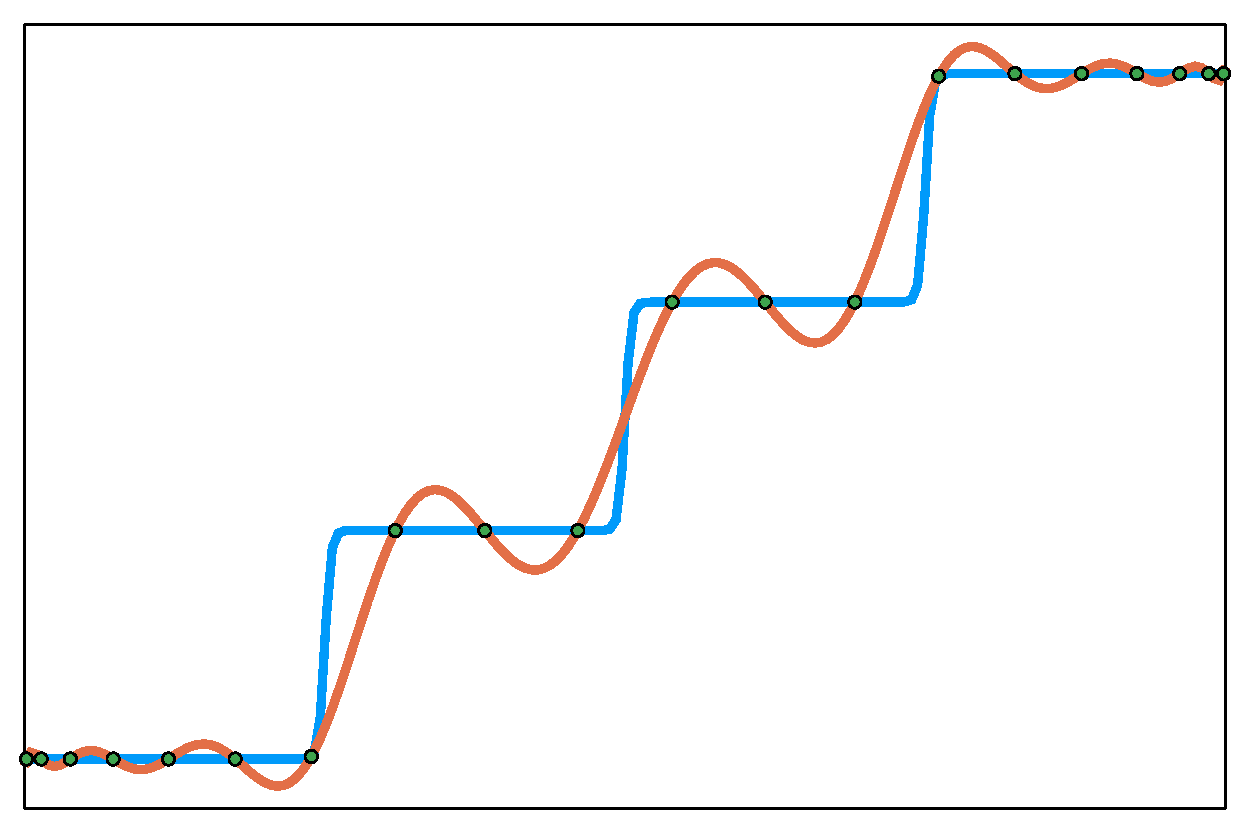
\includegraphics[width=.7\textwidth]{figures/chebychev_cover.pdf}
    % 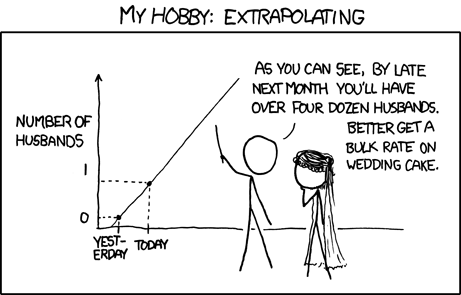
\includegraphics[width=.7\textwidth]{figures/extrapolating.png}
}
\author{%
    Urbain \textsc{Vaes} \\
    \texttt{urbain.vaes@nyu.edu}
}
\date{\vspace{1cm} {\large\textsc{NYU Paris}, Fall term 2022} \\[2cm]
    \vfill
    \flushleft \textbf{Weekly schedule}:
    \begin{itemize}
        \item Lectures on Monday and Wednesday from 15:00 to 16:15 (Paris time) in room 406;
        \item Recitation on Wednesday from 16:30 to 18:00 (Paris time) in room 406;
        \item Office hour on Thursday at 10:00 (Paris time).
    \end{itemize}
}

\maketitle


\frontmatter
\chapter*{License}%
\label{cha:license}

The copyright of these notes rests with the author and
their contents are made available under a Creative Commons
\href{https://creativecommons.org/licenses/by-sa/4.0/}{``Attribution-ShareAlike 4.0 Interational''}
license.
You are free to copy, distribute, transform and build upon the course material under the following terms:
\begin{itemize}
    \item \textbf{Attribution.}
    You must give appropriate credit, provide a link to the license, and indicate if changes were made.
    You may do so in any reasonable manner, but not in any way that suggests the licensor endorses you or your use.
    \item \textbf{ShareAlike.} If you remix, transform, or build upon the material,
        you must distribute your contributions under the same license as the original.
\end{itemize}

\vspace{1cm}
\hfill 
\includegraphics[scale=.7]{figures/cc-by-sa.pdf}

\chapter*{Course syllabus}%

\paragraph{Course content.}%
This course is aimed at giving a first introduction to classical topics in numerical analysis,
including floating point arithmetics and round-off errors,
the numerical solution of linear and nonlinear equations,
iterative methods for eigenvalue problems,
interpolation and approximation of functions,
and numerical quadrature.
If time permits, we will also cover numerical methods for solving ordinary differential equations.

\paragraph{Prerequisites.}%
The course assumes a basic knowledge of linear algebra and calculus.
Prior programming experience in Julia, Python or a similar language is desirable but not required.

\paragraph{Study goals.}%
After the course,
the students will be familiar with the key concepts of \emph{stability}, \emph{convergence} and \emph{computational complexity} in the context of numerical algorithms.
They will have gained a broad understanding of the classical numerical methods available for performing fundamental computational tasks,
and be able to produce efficient computer implementations of these methods.

\paragraph{Education method.}%
The weekly schedule comprises two lectures (2$\times$ 1h15 per week) and an exercise session (1h30 per week).
The course material includes rigorous proofs as well as illustrative numerical examples in the Julia programming language,
and the weekly exercises blend theoretical questions and practical computer implementation tasks.

\paragraph{Assessment.}%
\label{par:assessment}
Computational coursework will be handed out on a biweekly basis,
each of them focusing on one of the main topics covered in the course.

\paragraph{Literature and study material.}%
A comprehensive reference for this course is the following textbook:~\fullcite{MR2265914}.
Other pointers to the literature will be given within each chapter.


\iftitleincluded
\tableofcontents
\fi

\mainmatter
\chapter*{Introduction}%
In a wide variety of scientific disciplines,
ranging from physics to biology and economics,
the phenomena under consideration are well-described by mathematical equations.
More often than not,
these equations are too difficult to be solved analytically,
and so one has to recur to \emph{computer calculations} in order to obtain approximate solutions.
Practical applications in which computer simulation plays a crucial role include
weather forecasting, drug discovery through molecular modeling,
flight simulation, and structural engineering, to mention just a few.

% Since computers have finite memory,
% they are not able to store
% continuous mathematical objects,
% such as solutions to partial differential equations, are represented using finite arrays of numbers,
% which introduces an approximation error.
% When approximating
% It is important to understand the error induced by the use of numerical simulation,
% As application domains where computer simulation is particularly important,
% we mention weather forecasting

Numerical simulation may also be employed in order to calibrate mathematical models of physical phenomena,
particularly when observation through experiment is impractical or too costly.
For example, it is frequently the case that the parameters in mathematical models for turbulence are estimated not from real data,
but from synthetic data generated by computer simulation of the fundamental equations of fluid mechanics.
Relying on ``computer experiments'' is attractive in this context because
these enable to perform accurate measurements without disturbing the system being observed.
Numerical simulation is also very useful to understand and build simplified models for physical phenomena at very small scales,
where direct observation is beyond the current capabilities of experimental physics.

The aim of this course is to present the standard numerical methods for performing the tasks most commonly encountered in applications:
the solution of linear and nonlinear systems of equations,
the solution of eigenvalue problems,
interpolation and approximation of functions,
and numerical integration.
For a given task,
there are usually many numerical methods to choose from,
and these often include parameters which must be fixed appropriately in order to guarantee a good efficiency.
In order to understand what method to employ for best results according to the context,
we study carefully the \emph{convergence properties} of the methods considered.
Six topics will be covered in these lecture notes.
\begin{itemize}
    \item
        \textbf{Floating point arithmetic.}
        In~\cref{cha:rounding_errors},
        we discuss how real numbers are represented, manipulated and stored on a computer.
        There is an uncountable infinity of real number,
        but only a finite subset of these can be represented exactly on a computer.
        This subset is specified in the~\emph{IEEE 754} standard,
        which is widely accepted today and employed in most programming languages, including \texttt{Julia}.

    \item
        \textbf{Solution of linear systems.}
        In \cref{cha:solution_of_linear_systems},
        we study the most widely-used numerical methods for solving linear systems.
        Linear systems are ubiquitous in science,
        often arising from the discretization of linear elliptic partial differential equations,
        which themselves govern a large number of physical phenomena including heat propagation, electromagnetism, gravitation and the deformation of solids.
        % using for example a finite difference method.
        A subclass of linear systems, in which the matrix on the left-hand side is positive semi-definite,
        also appear in the context of optimization:
        indeed, if $A \in \real^{n \times n}$ is positive definite and $b \in \real^n$,
        then the unique minimizer of $\frac{1}{2} x^\t A x - b^\t x$ satisfies the linear system $A x = b$.

    \item
        \textbf{Solution of nonlinear equations.}
        In \cref{cha:solution_of_nonlinear_systems},
        we present widely-used methods for solving nonlinear equations.
        Like linear equations, nonlinear equations are omnipresent in science,
        a prime example being the Navier--Stokes equation describing the motion of fluid flows.
        They are usually much more difficult to solve and require dedicated techniques.
        In addition, the solution to nonlinear equations usually rarely admit analytical expressions;
        they need to be approximated using iterative methods.

    \item
        \textbf{Solution of eigenvalue problems.}
        In \cref{cha:numerical_computation_of_eigenvalues},
        we present and study the standard methods for calculating the eigenfunctions and eigenvalues of a matrix.
        Eigenvalue problems have a large number of applications,
        for instance in quantum physics and vibration analysis.
        They are also at the root of the PageRank algorithm for ranking web pages,
        which played a key role in the early success of Google search.

    \item
        \textbf{Interpolation and extrapolation of functions.}
        In \cref{cha:interpolation_and_approximation},
        we focus on the topics of interpolation and approximation.
        \emph{Interpolation} is concerned with the construction of a function within a class,
        for example the set of polynomials,
        under the constraint that the function takes given values when evaluated at a discrete set of points.
        The aim of \emph{approximation}, on the other hand,
        is usually to determine, within a class of simple functions,
        which one is closest to a given function.
        Depending on the metric employed to measure closeness,
        this may or may not be a well-defined problem.

    \item
        \textbf{Numerical integration.}
        In~\cref{cha:quadrature},
        we study numerical methods for computing definite integrals.
        This chapter is strongly related to the previous one,
        as numerical approximations of the integral of a function are often obtained by first approximating the function,
        say by a polynomial, and then integrating the approximation exactly.
\end{itemize}

% Throughout the course, the \texttt{Julia} programming language is employed to exemplify the concepts.


\chapter{Floating point arithmetic}%
\label{cha:rounding_errors}
\minitoc

\section*{Introduction}%
\label{sec:introduction}
% In numerical simulation,
% errors arise from four distinct sources:
% \begin{itemize}
%     \item
%         The \emph{modeling error} accounts for the mismatch between reality and the mathematical equations describing it.
%         Mathematical equations are generally only an approximation of reality.
%     \item
%         The \emph{numerical error}
%         refers to the error introduced by numerical methods,
%         which are generally not exact;
%         they only provide approximate solutions to the mathematical equations.
%     \item
%         The \emph{roundoff errors} come from the fact that
%         computers are unable to store the majority of real numbers exactly.
%         The number $\pi$, for example,
%         contains an infinite amount of digits
% \end{itemize}

When we study numerical algorithms in the next chapters,
we assume implicitly that the operations involved are performed exactly.
On a computer, however, only a subset of the real numbers can be stored and,
consequently, many arithmetic operations are performed only approximately.
This is the source of the so-called \emph{round-off errors}.
The rest of this chapter is organized as follows.
\begin{itemize}
    \item
        In \cref{sec:binary_representation_of_real_numbers},
        we briefly discuss the binary representation of real numbers.
    \item
        In \cref{sec:set_of_values},
        we describe the set of floating point numbers that can be represented in the usual floating point formats;
    \item
        In \cref{sec:arithmetic_operations_between_floating_point_formats}
        we explain how arithmetic operations between floating point numbers behave.
        We insist in particular on the fact that,
        in a calculation involving several successive arithmetic operations,
        the result of each intermediate operation is stored as a floating point number,
        with a possible error.
        % This is why \texttt{1.0 + 1e-100 - 1.0} returns \texttt{0.0},
        % in the usual double-precision format.
    \item
        In \cref{sec:encoding_of_floating_point_numbers},
        we briefly present how floating point numbers are encoded
        according to the IEEE 754 standard, widely accepted today.
        We discuss also the encoding of special values such as \texttt{Inf}, \texttt{-Inf} and \texttt{NaN}.
\end{itemize}
In order to completely describe a floating-point system,
one would in principle need to also discuss the storage of integer numbers
and the conversion mechanisms between different number formats,
as well as a number of edge cases.
For instance, the reference IEEE 754 standard specifies that \texttt{NaN == NaN} must evaluate to \texttt{false},
which is somewhat arbitrary but may be useful in some situations.
Needless to say,
a comprehensive discussion of the subject is beyond the scope of this course;
our aim in this chapter is only to introduce the key concepts.

\section{Binary representation of real numbers}%
\label{sec:binary_representation_of_real_numbers}

Given any integer number $\beta > 0$, called the \emph{base},
a real number $x$ can always be expressed as a finite or infinite series of the form
\begin{equation}
    \label{eq:base_representation}
    x = (-1)^s \sum_{k=-n}^{\infty} a_k \beta^{-k}, \qquad 0 \leq a_k < \beta.
\end{equation}
The number $x$ may then be denoted as $(-1)^s (a_{-n} a_{-n+1}\dots a_{-1} a_{0}.a_{1} a_{2} \dots)_{\beta}$,
where the subscript $\beta$ indicates the base and $s \in \{0, 1\}$ encodes the sign.
This numeral system is called the \emph{positional notation} and is universally used today,
both by humans (usually with $\beta=10$) and machines (usually with $\beta=2$).
If the base~$\beta$ is omitted,
it is always assumed that $\beta = 10$ unless otherwise specified
-- this is the \emph{decimal} representation.
% It is likely that the prevalence of base 10 in human writing is a consequence of human morphology,
% although this fact has not been demonstrated by historians.
In computer science, several bases other than 10 are regularly employed,
for example the following:
\begin{itemize}
    \item
        Base 2 (binary) is the usual choice for storing numbers on a machine.
        The binary format is convenient because the digits have only two possible values, 0 or 1,
        and so they can be stored using simple electrical circuits with two states.
        We employ the binary notation extensively in the rest of this chapter.
        Notice that, just like multiplying and dividing by~10 is easy in base 10,
        multiplying and dividing by 2 is very simple in base 2:
        these operations amount to shifting all the bits by one position to the left or right,
        respectively.

    \item
        Base 16 (hexadecimal) is sometimes convenient to represent numbers in a compact manner.
        In order to represent the values 0-15 by a single digit,
        16 different symbols are required, which are conventionally denoted by $\{0,1,2,3,4,5,6,7,8,9,A,B,C,D,E,F\}$.
        With this notation, we have $(FF)_{16} = (255)_{10}$, for example.

        The hexadecimal notation is often used in programming languages for describing colors specified by a triplet $(r,g,b)$ of values between 0 and 255,
        corresponding to the primary colors \emph{red}, \emph{blue} and \emph{green}.
        Since the number of possible values for the components is $256 = 16^2$,
        only 2 digits are required to represent these in the hexadecimal notation.
        Hexadecimal numbers are also employed in IPv6 addresses.
\end{itemize}

\subsection{Conversion between binary and decimal formats}%
Obtaining the decimal representation of a binary number can be achieved from~\eqref{eq:base_representation},
using the decimal representations of the powers of 2.
Since all the positive and negative powers of 2 have finite decimal representations,
any real number with a finite representation in base 2 has a finite representation also in base 10.
For example, $(0.01)_2 = (0.25)_{10}$ and $(0.111)_2 = (0.875)_{10}$.
\begin{example}
    [Converting a binary number to decimal notation]
    \label{example:converting_binary_to_decimal}
    Let us calculate the decimal representation of $x = (0.\overline{10})_2$,
    where the horizontal line indicates repetition: $x = (0.101010\dots)_2$.
    By definition, it holds that
    \[
        x = \sum_{k=0}^{\infty} a_k 2^{-k},
    \]
    where $a_k = 0$ if $k$ is even and 1 otherwise.
    Thus, the series may be rewritten as
    \[
        x = \sum_{k=0}^{\infty} 2^{-(2k+1)} = \frac{1}{2} \sum_{k=0}^{\infty} (2^{-2})^k.
    \]
    We recognize on the right-hand side a geometric series with common ratio $r = 2^{-2} = \frac{1}{4}$,
    and so we obtain
    \[
        x = \frac{1}{2} \left( \frac{1}{1-r} \right) = \frac{2}{3} = (0.\overline 6)_{10}.
    \]
\end{example}

Obtaining the binary representation of a decimal number is more difficult,
because negative powers of 10 have \emph{infinite} binary representations,
as \cref{exercise:binary_zero_point_one} demonstrates.
There is, however, a simple procedure to perform the conversion,
which we present for the specific case of a real number $x$ with decimal representation of the form $x = (0.a_1\dots a_n)_{10}$.
In this setting,
the bits~$(b_1, b_2, \dots)$ in the binary representation of $x = (0.b_1b_2b_2 \dots)_2$ may be obtained as follows:
\begin{algorithm}
\caption{Conversion of a number to binary format}%
\label{algo:conversion_to_binary}%
\begin{algorithmic}[1]
\State $i \gets 1$
\While{$x \neq 0$}
    \State $x \gets 2x$%
    \label{line:after_while}
    \If{$x \geq 1$}
        \State $b_i \gets 1$
    \Else
        \State $b_i \gets 0$
    \EndIf
    \State $x \gets x - b_i 2^{-i}$
    \State $i \gets i+1$
\EndWhile
\end{algorithmic}
\end{algorithm}

\begin{example}
    [Converting a decimal number to binary notation]
    Let us calculate the binary representation of $x = \frac{1}{3} = (0.\overline{3})_{10}$.
    We apply~\cref{algo:conversion_to_binary} and collate the values of $i$ and $x$ obtained at the beginning of each iteration,
    i.e.\ just before~\cref{line:after_while}, in the table below.
    \begin{center}
    \begin{tabular}{|c|c|c|}
        \hline
        $i$ & $x$ & Result \\ \hline
        $1$ & $\frac{1}{3}$ & 0.\textbf{0}000\dots \\ \hline
        $2$ & $\frac{2}{3}$ & 0.0\textbf{1}00\dots \\ \hline
        $3$ & $\frac{1}{3}$ & 0.00\textbf{0}0\dots \\ \hline
    \end{tabular}
    \end{center}
    Since $x$ in the last row is again $\frac{1}{3}$,
    successive bits alternate between 0 and 1,
    and the binary representation of $x$ is given by $(0.\overline{01})_2$.
    This is not surprising since $2x = (0.66)_{10} = (0.\overline{10})_2$,
    as we saw in~\cref{example:converting_binary_to_decimal}.
\end{example}

\subsection{Exercises}%

\begin{exercise}
    \label{exercise:non_unique_representation}
    Show that if a number $x \in \real$ admits a finite representation~\eqref{eq:base_representation} in base $\beta$,
    then it also admits an infinite representation.
    \textbf{Hint:} You may have learned before that $(0.\overline 9)_{10} = 1$.
\end{exercise}

\begin{exercise}
    How many digits does it take to represent all the integers from 0 to $10^{10} - 1$ in decimal and binary format?
    What about the hexadecimal format?
\end{exercise}

\begin{exercise}
    Find the decimal representation of $(0.000\overline{1100})_2$.
\end{exercise}

\begin{exercise}
    \label{exercise:binary_zero_point_one}
    Find the binary representation of $(0.1)_{10}$.
\end{exercise}

\begin{exercise}
    Implement~\cref{algo:conversion_to_binary} on a computer and verify that it works.
    Your function should take as argument an array of integers containing the digits after the decimal point;
    that is, an array of the form \verb?[a_1, ..., a_n]?.
\end{exercise}

\begin{exercise}
    As mentioned above, \cref{algo:conversion_to_binary} works only for decimal numbers of the specific form~$x = (0.a_1\dots a_n)_{10}$.
    Find and implement a similar algorithm for integer numbers of the form $x = (a_{-n} \dots a_{0})_{10}$.
\end{exercise}

\section{Set of values representable in floating point formats}%
\label{sec:set_of_values}
We mentioned in the introduction that,
because of memory limitations,
only a subset of the real numbers can be stored exactly in a computer.
Nowadays, the vast majority of programming languages and software comply with the IEEE 754 standard,
which requires that the set of representable numbers be of the form
\begin{align}
    \notag
    \floating (p, E_{\min}, E_{\max})
    = \Bigl\{ & (-1)^s 2^E (b_0. b_1 b_2 \dots b_{p-1})_2 \colon \\
    \label{eq:number_format}%
              & \qquad s \in \{0, 1\}, b_i \in \{0, 1\} \, \text{and} \, E_{\min} \leq E \leq E_{\max} \Bigr\}.
\end{align}
In addition to these, floating number formats provide the special entities \texttt{Inf}, \texttt{-Inf} and \texttt{NaN},
the latter being an abbreviation for \emph{Not a Number}.
Three parameters appear in the set definition~\eqref{eq:number_format}.
The parameter $p \in \nat_{>0}$ is the number of significant bits (also called the precision),
and $(E_{\min}, E_{\max}) \in \integer^2$ are respectively the minimum and maximum exponents.
From the precision, the \emph{machine epsilon} is defined as $\varepsilon_{M} = 2^{-p-1}$;
its significance is discussed in~\cref{sub:relative_error_and_epsilon_machine}.

For a number $x \in \floating(p, E_{\min}, E_{\max})$,
$s$ is called the \emph{sign}, $E$ is the \emph{exponent} and
$b_0. b_1 b_2 \dots b_{p-1}$ is the \emph{significand}.
The latter can be divided into a \emph{leading bit} $b_0$ and the \emph{fraction} $b_1 b_2 \dots b_{p-1}$,
to the right of the binary point.
The most widely used floating point formats are the \emph{single} and \emph{double precision} formats,
which are called respectively \texttt{Float32} and \texttt{Float64} in Julia.
Their parameters,
together with those of the lesser-known half-precision format,
are summarized in~\cref{table:floating_point_formats}.
In the rest of this section we use the shorthand notation $\floating_{32}$ and $\floating_{64}$.
Note that $\floating_{32} \subset \floating_{64}$.
\begin{table}[ht]
    \centering
    \begin{tabular}{|c|c|c|c|}
        \hline
        & Half precision & Single precision & Double precision
        \\ \hline
        $p$ & 11 & 24 & 53
        \\ \hline
        $E_{\min}$ & -14 & -126 & -1022
        \\ \hline
        $E_{\max}$ & 15 & 127 & 1023
        \\ \hline
    \end{tabular}
    \caption{%
        Floating point formats.
        The first column corresponds to the \emph{half-precision} format.
        This format,
        which is available through the \texttt{Float16} type in Julia,
        is more recent than the single and double precision formats.
        It was introduced in the 2008 revision to the IEEE 754 standard of 1985,
        a revision known as IEEE 754-2008.
    }%
    \label{table:floating_point_formats}
\end{table}

\begin{remark}
    Some definitions,
    notably that in~\cite[Section 2.5.2]{MR2265914},
    include a general base~$\beta$ instead of the base 2
    as an additional parameter in the definition of the number format~\eqref{eq:number_format}.
    Since the binary format ($\beta = 2$) is always employed in practice,
    we focus on this case for simplicity in most of this chapter.
\end{remark}

\subsection{Making the floating point representation unique}%
\label{sub:defining_a_unique_representation}

Given a real number $x \in \floating (p, E_{\min}, E_{\max})$,
the exponent $E$ and significand  are generally not uniquely defined.
For example, the number $2.0 \in \floating_{64}$ may be expressed as $(-1)^0 2^1 (1.00\dots00)_2$ or, equivalently, as $(-1)^0 2^{2} (0.100\dots00)_2$.
To remove this ambiguity,
one may define the \emph{standard representation} of a number by requiring that
\begin{itemize}
    \item either $E > E_{\min}$ and $b_0 = 1$;
    \item or $E = E_{\min}$, in which case the leading bit may be 0.
\end{itemize}
The following result proves that these rules define the exponent and significand uniquely.
\begin{proposition}
    \label{prop:uniqueness_standard_representation}
    Assume that
    \begin{equation}
        \label{eq:equality_floating_point}
        (-1)^s (2^{E} b_0.b_1\dots b_{p-1})_2 = (-1)^{\widetilde s} (2^{\widetilde E} \widetilde b_0. \widetilde b_1\dots \widetilde b_{p-1})_2,
    \end{equation}
    where the parameter sets $(s, E, b_0, \dots b_{p-1})$ and $(\widetilde s, \widetilde E, \widetilde b_0, \dots, \widetilde b_{p-1})$ both satisfy the above rule.
    Then $E = \widetilde E$ and $b_i = \widetilde b_i$ for $i \in \{0, \dots, p-1\}$.
\end{proposition}
\begin{proof}
    We show that $E = \widetilde E$,
    after which the equality of significands follows trivially,
    Let us assume for contradiction that $E > \widetilde E$
    and denote the left and right-hand sides of~\eqref{eq:equality_floating_point} by~$x$ and~$\widetilde x$, respectively.
    Then~$E > E_{\min}$, implying that $b_0 = 1$ and so $2^{E} \leq |x| < 2^{E+1}$.
    On the other hand, it holds that $|\widetilde x| < 2^{\widetilde E+1}$ regardless of whether $\widetilde E = E_{\min}$ or not.
    Since $E \geq \widetilde E + 1$ by assumption,
    we deduce that $|\widetilde x| < 2^E \leq |x|$,
    which contradicts the equality $x = \widetilde x$.
\end{proof}

In view of \cref{prop:uniqueness_standard_representation},
we can talk without ambiguity about \emph{the} exponent or \emph{the} significand of a number in $\floating (p, E_{\min}, E_{\max})$,
the standard representation being implicitly assumed.
A floating point number whose standard representation has a leading bit equal to 1 is called \emph{normalized},
whereas one with a leading bit equal to zero is called \emph{subnormal} or \emph{denormalized}.
We give more information on this subject in~\cref{sec:encoding_of_floating_point_numbers},
which is devoted specifically to the encoding of floating point numbers.

% In a computer, however, each number in a floating point format is always represented in the same manner,
% which is useful in order to perform comparisons:
% since the representation is unique,
% two numbers are equal if only if their sign, exponent and significand are equal.

\begin{remark}
    [Nonuniqueness of the floating point represention of 0.0]
    The sign $s$ is clearly unique for any number in a floating point format,
    except for $0.0$,
    which could in principle be represented as
    \[
        (-1)^0 2^{E_{\min}} (0.00\dots00)_2
        \qquad \text{or} \qquad
        (-1)^1 2^{E_{\min}} (0.00\dots00)_2.
    \]
    In practice, both representations of 0.0 are available on most machines,
    and these behave slightly differently.
    For example $\texttt{1/(0.0) = Inf}$ but $\texttt{1/(-0.0) = -Inf}$.
\end{remark}

In \texttt{Julia}, non-integer numbers are interpreted as \julia{Float64} by default,
which you may verify by using the \julia{typeof} function.
For example, the instruction ``\julia{a = 0.1}'' is equivalent to~``\julia{a = Float64(0.1)}''.
In order to define a number of type \julia{Float32},
the suffix $\julia{f0}$ must be appended to the decimal expansion.
For instance, the instruction ``$\julia{a = 4.0f0}$'' defines a floating point number~\julia{a} of type \julia{Float32};
it is equivalent to ``\julia{a = Float32(4.0)}''.

\subsection{Relative error and machine epsilon}%
\label{sub:relative_error_and_epsilon_machine}
Let $x$ be a nonzero real number and $\widehat x$ be an approximation.
We define the absolute and relative errors of the approximation as follows.
\begin{definition}
    [Absolute and relative error]
    The absolute error is given by $|x - \widehat x|$,
    whereas the relative error is
    \[
        \frac{|x - \widehat x|}{|x|}
    \]
\end{definition}

The following result establishes a link between the machine $\varepsilon_M$ and
the relative error between a real number and the closest member of a floating point format.
\begin{proposition}
    \label{prop:relative_error_and_machine_epsilon}
    Let $x_{\min}$ and $x_{\max}$ denote the smallest and largest \emph{normalized} positive numbers in a format $F = \floating(p, E_{\min}, E_{\max})$.
    If $x \in [-x_{\max}, -x_{\min}] \cup [x_{\min}, x_{\max}]$,
    then there exists $\widehat x \in \floating(p, E_{\min}, E_{\max})$ such that
    \begin{equation}
        \label{eq:bound_epsilon_machine}
        \min_{\widehat x \in F} \frac{|x - \widehat x|}{|x|} \leq \frac{1}{2} 2^{-(p-1)}
        = \frac{1}{2} \varepsilon_M.
    \end{equation}
\end{proposition}
\begin{proof}
    For simplicity, we also assume that $x > 0$.
    Let us introduce $n = \lfloor \log_2(x) \rfloor$ and $y := 2^{-n} x$.
    Since $y \in [1, 2)$,
    it has a binary representation of the form
    \(
        (1.b_1 b_2\dots)_2,
    \)
    where the bits after the binary point are not all equal to 1 ad infinitum.
    Thus
    \(
        x = 2^{n} (1.b_1 b_2\dots)_2,
    \)
    and from the assumption that $x_{\min} \leq x \leq x_{\max}$
    we deduce hat $E_{\min} \leq n \leq E_{\max}$.
    % \footnote{%
    %     The inequality here is strict,
    %     because $2^{E_{\min} - 1} (1.\overline{1})_2 = 2^{E_{\min}} = x_{\min}$.
    %     Remember that the binary expansion of a real number is generally not unique!
    %     See~\cref{exercise:non_unique_representation}.
    % }
    % which is excluded by assumption.
    We now define the number $x_- \in F$ by truncating the binary expansion of $x$ as follows:
    \[
        x_- = 2^n (1.b_1 \dots b_{p-1})_2.
    \]
    The distance between $x_-$ and its successor in $F$,
    which we denote by $x_+$, is given by $2^{n-p+1}$.
    Consequently, it holds that
    \[
        (x_+ - x) + (x-x_-) = x_+ - x_- = 2^{n-p+1}.
    \]
    Since both summands on the left-hand side are positive,
    this implies that either $x_+ - x$ or $x - x_-$ is bounded from above by $\frac{1}{2} 2^{n-p+1} \leq \frac{1}{2} 2^{-p+1}x$,
    which concludes the proof.
\end{proof}

The machine epsilon can be viewed as the maximum relative difference between a normalized floating point number $x$ and its successor,
defined as the smallest number in the floating point format that is strictly larger than $x$.

\Cref{fig:float64_density} depicts the density of double-precision floating point numbers,
i.e.\ the number of~$\floating_{64}$ members per unit on the real line.
The figure shows that the density decreases as the absolute value of $x$ increases.
We also notice that the density is piecewise constant with discontinuities at powers of 2;
each discontinuity corresponds to a change of exponent in the standard representation.
\Cref{fig:float64_spacing} illustrates the relative spacing between successive floating point numbers,
in units of machine precision.
Although the absolute spacing increases with the absolute value of $x$,
the relative spacing oscillates between~$\frac{1}{2} \varepsilon_{M}$ and~$\varepsilon_M$.

\begin{figure}
    \centering
    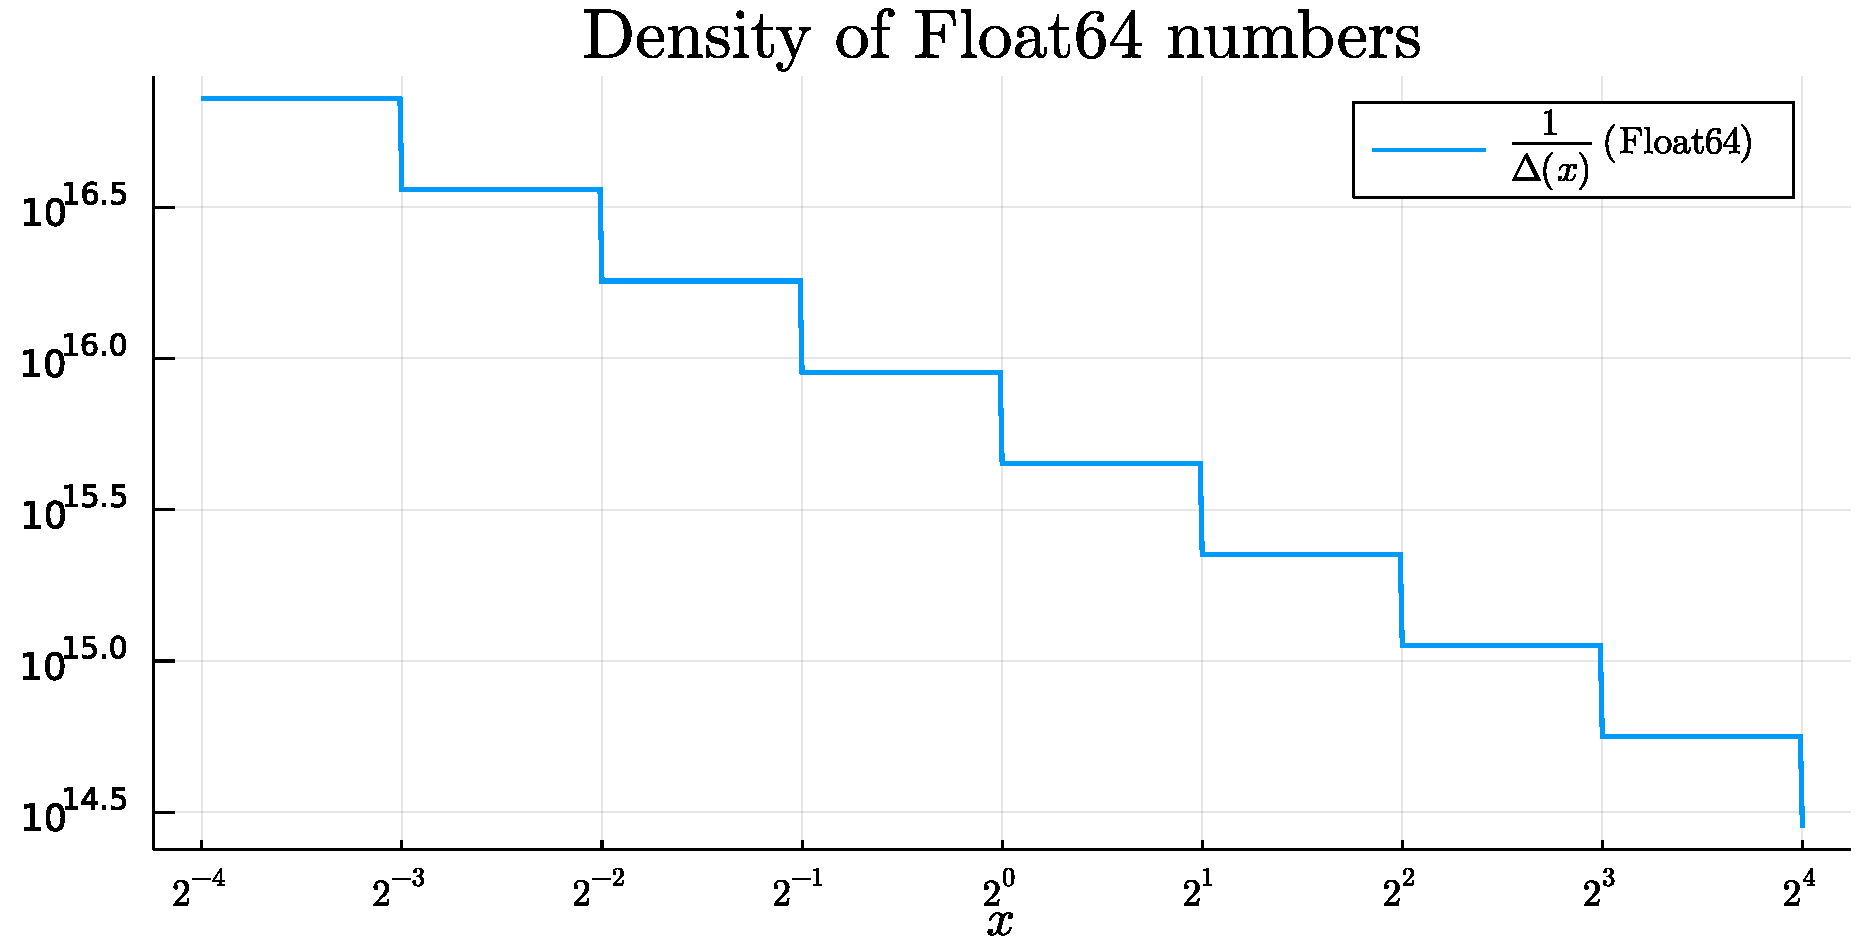
\includegraphics[width=.8\textwidth]{figures/float64_density.pdf}
    \caption{%
        Density of the double-precision floating point numbers,
        measured here as~$1/\Delta(x)$ where,
        for $x \in \floating_{64}$,
        $\Delta(x)$ denotes the distance between $x$ and its successor in $\floating_{64}$.
    }%
    \label{fig:float64_density}%
\end{figure}

\begin{figure}[ht]
    \centering
    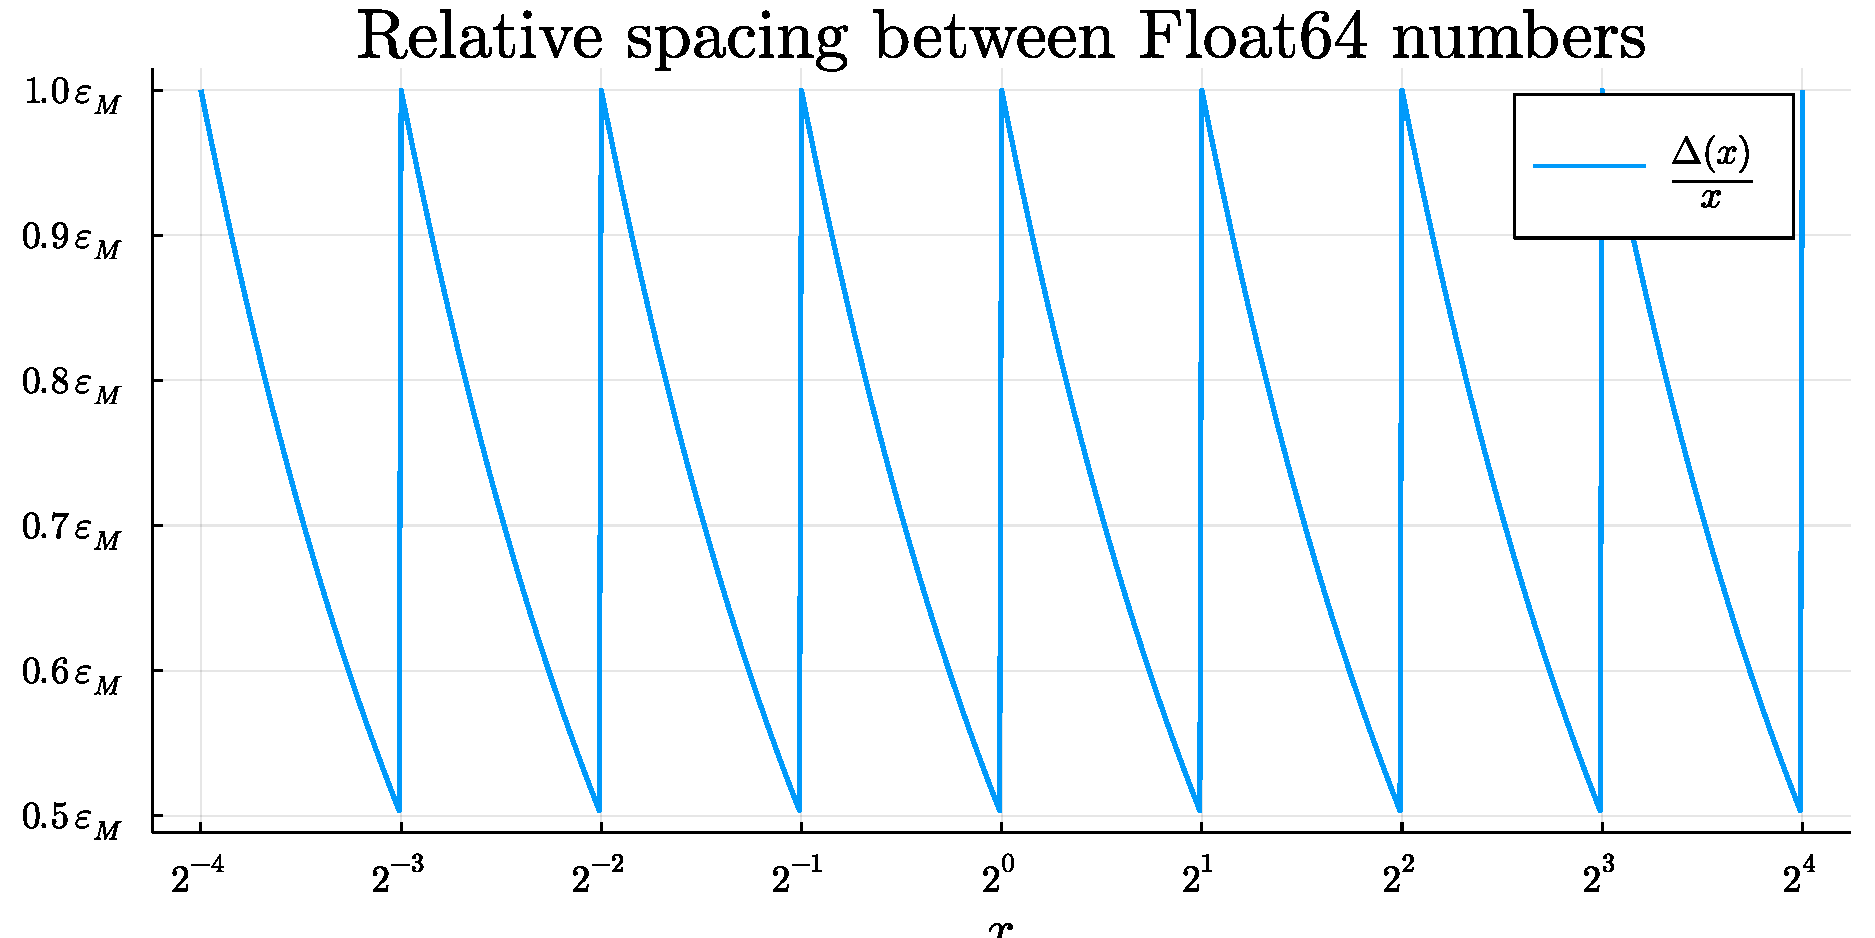
\includegraphics[width=.8\textwidth]{figures/float64_spacing.pdf}
    \caption{%
        Relative spacing between successive double-precision floating point numbers in the ``normal range''.
        The relative spacing oscillates between $\frac{1}{2} \varepsilon_M$ and $\varepsilon_M$.
    }%
    \label{fig:float64_spacing}
\end{figure}

The picture of the relative spacing between successive floating point numbers looks quite different for denormalized numbers.
This is illustrated in \cref{fig:float64_spacing_denormalized},
which shows that the relative spacing increases beyond the machine epsilon in the denormalized range.
Fortunately, in the usual $\floating_{32}$ and $\floating_{64}$ formats,
the transition between normalized and denormalized numbers occurs at such a small value that
it rarely needs worrying about.

\begin{figure}[ht]
    \centering
    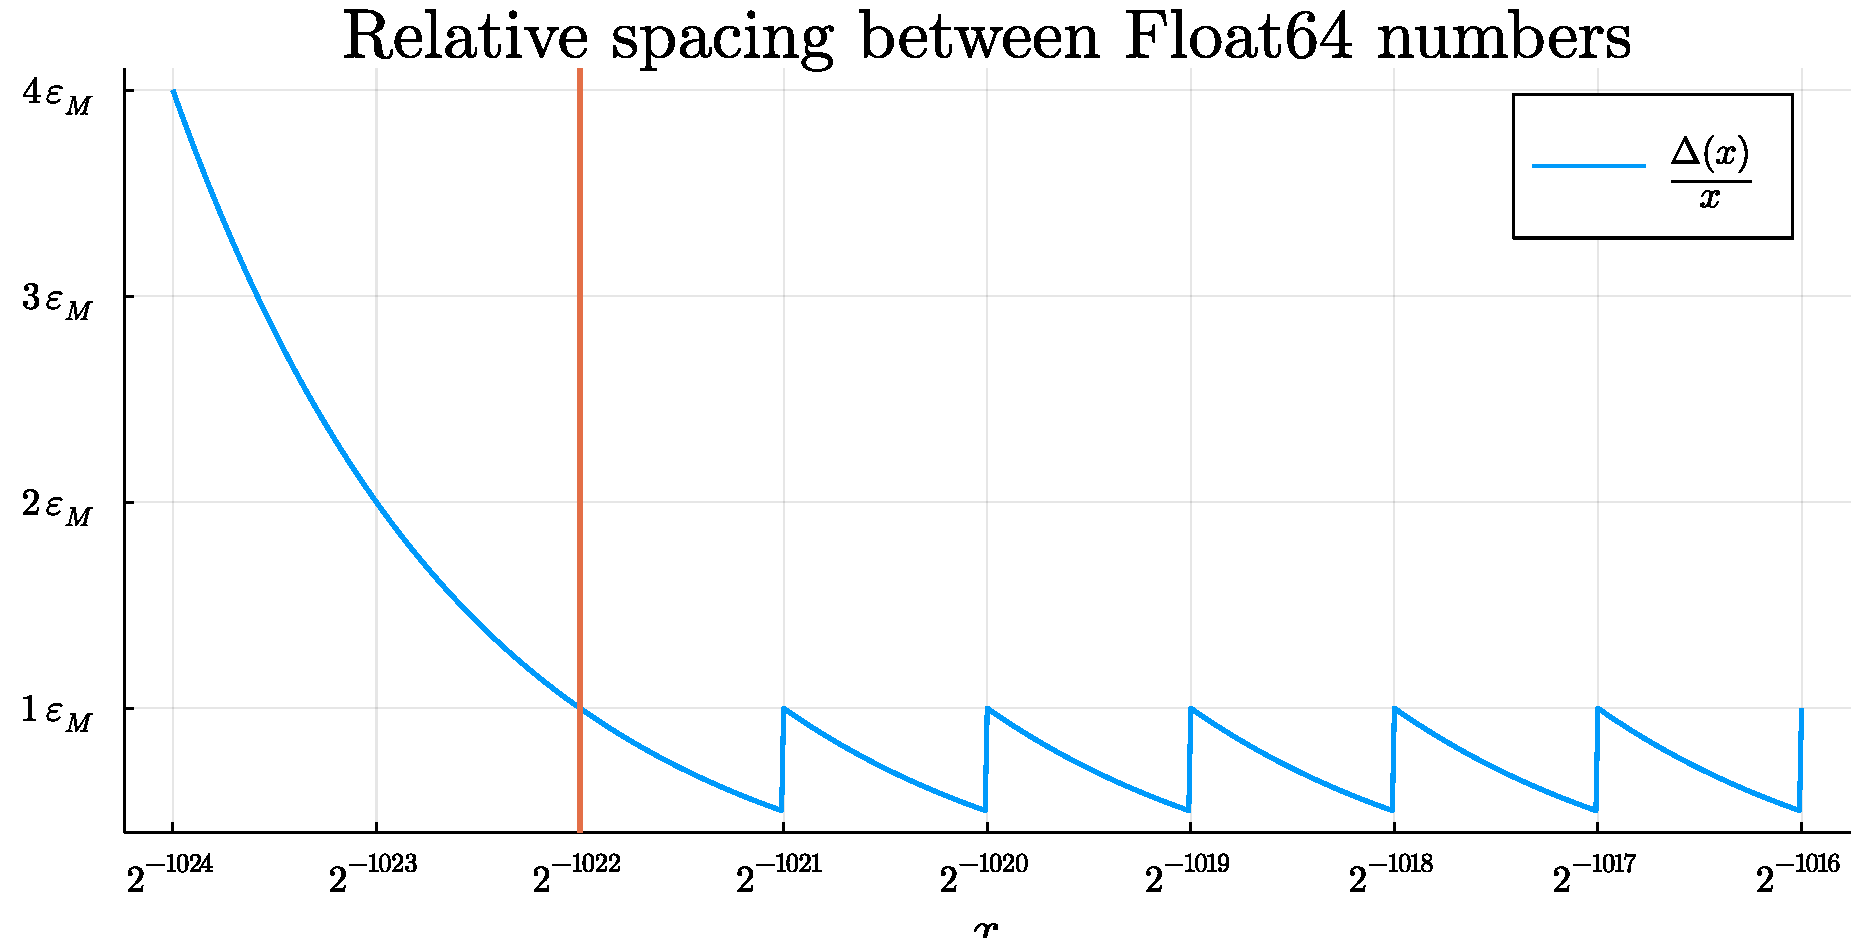
\includegraphics[width=.8\textwidth]{figures/float64_spacing_denormalized.pdf}
    \caption{%
        Relative spacing between successive double-precision floating point numbers,
        over a range which includes denormalized number.
        The vertical red line indicates the transition from denormalized to normalized numbers.
    }%
    \label{fig:float64_spacing_denormalized}
\end{figure}

\begin{remark}
    In Julia,
    the machine epsilon can be obtained using the \texttt{eps} function.
    For example, the instruction \julia{eps(Float16)} returns $\varepsilon_M$ for the half-precision format.
\end{remark}

\subsection{Exercises}%

\begin{exercise}
    Write down the values of the smallest and largest, in absolute value,
    positive real numbers representable in the $\floating_{32}$ and $\floating_{64}$ formats.
\end{exercise}

\begin{exercise}
    [Relative error and machine epsilon]
    \label{exercise:machine_epsilon}
    Prove that the inequality~\eqref{eq:bound_epsilon_machine} is sharp.
\end{exercise}

\begin{exercise}
    [Cardinality of the set of floating point numbers]
    Show that, if $E_{\max} \geq E_{\min}$, then $\floating(p, E_{\min}, E_{\max})$ contains exactly
    \[
        (E_{\max} - E_{\min}) 2^{p} + 2^{p+1} - 1
    \]
    \emph{distinct real numbers}.
    (In particular, the special values \texttt{Inf}, \texttt{-Inf} and \texttt{NaN} are not counted.)
    \textbf{Hint:} Count first the normalized and then the denormalized numbers.
\end{exercise}

\section{Arithmetic operations between floating point formats}%
\label{sec:arithmetic_operations_between_floating_point_formats}

Now that we have presented the set of values representable on a computer,
we attempt in this section to understand precisely how arithmetic operations between floating point formats are performed.
The key mechanism governing arithmetic operations on a computer is that of \emph{rounding},
the action of approximating a real number regarded as infinitely precise by a number in a floating point format $\floating (p, E_{\min}, E_{\max})$.
The IEEE 754 standard specifies stipulates that the default mechanism for rounding a real number $x$,
called \emph{round to nearest, ties to even},
should behave as follows:
\begin{itemize}
    \item
        \textbf{Standard case}:
        The number $x$ is rounded to the \emph{nearest representable number},
        if this number is unique.
    \item
        \textbf{Edge case}:
        When there are two equally near representable numbers in the floating point format,
        the one with the least significant bit equal to zero is delivered.
    \item
        \textbf{Infinities}:
        If the real number $x$ is larger than the largest representable number in the format,
        that is larger than or equal to $x_{\max} = 2^{E_{\max}} (2 - 2^{-p-1})$,
        then there are two cases,
        \begin{itemize}
            \item If $x < 2^{E_{\max}} (2 - 2^{-p})$, then $x_{\max}$ is delivered;
            \item Otherwise, the special value~\texttt{Inf} is delivered.
        \end{itemize}
        In other words, $x_{\max}$ is delivered if it would be delivered by following the rules of the first two bullet points
        in a different floating point format with the same precision but a larger exponent $E_{\max}$.
        A similar rule applies for large negative numbers.
\end{itemize}

When a binary arithmetic operation ($+$, $-$, $\times$, $/$) is performed on floating point numbers in format $\floating$,
the result delivered by the computer is equal the exact result of the operation,
rounded according to the rules given above.
In other words,
the arithmetic operation is performed as if the computer first calculated an intermediate exact result,
and then rounded this intermediate result in order to provide a final result in $\floating$.

Mathematically,
arithmetic operations between floating point numbers in a given format $\floating$ may be formalized by introducing
the rounding operator ${\rm fl}: \real \to \floating$ and
by defining , for any binary operation $\circ \in \{+, -, \times, /\}$,
the corresponding machine operation
\[
    \widehat \circ\colon \floating \times \floating \rightarrow \floating; (x, y) \mapsto {\rm fl}(x \circ y).
\]
We defined this operator for arguments in the same floating point format~$\floating$.
If the arguments of a binary arithmetic operation are of different types,
the format of the end result,
known as the \emph{destination format},
depends on that of the arguments:
as a rule of thumb,
it is given by the most precise among the formats of the arguments.
In addition, recall that a floating point literal whose format is not explicitly specified is rounded to double-precision format
and so, for example, the addition \julia{0.1 + 0.1} produces the result ${\rm fl_{64}}\bigl(\rm fl_{64}(0.1) + \rm fl_{64}(0.1)\bigr)$,
where ${\rm fl}_{64}$ is the rounding operator to the double-precision format.

\begin{example}
    Using the \julia{typeof} function,
    we check that the floating point literal \texttt{1.0} is indeed interpreted as a double-precision number:
\begin{minted}{julia}
julia> a = 1.0; typeof(a)
Float64
\end{minted}

When two numbers in different floating point formats are passed to a binary operation,
the result is in the more precise format.
\begin{minted}{julia}
julia> typeof(Float16(1) + Float32(1))
Float32

julia> typeof(Float32(1) + Float64(1))
Float64
\end{minted}
\end{example}

If a mathematical expression contains several binary arithmetic operations to be performed in succession,
the floating point result of each intermediate calculation is stored in a floating point format dictated by the formats of its argument,
and this floating point number is employed in the next binary operation.
A consequence of this mechanism of arithmetic operations is that the operands $+$ and $*$ are generally \emph{not associative}.
For example, in general
\[
    (x \madd y) \madd  z \neq x \madd (y \madd z)
\]
\begin{example}
    Let $x = 1$ and $y = 3 \times 2^{-13}$.
    Both of these numbers belong to $\floating_{16}$ and,
    denoting by $\widehat +$ machine addition in~$\floating_{16}$,
    we have
    \begin{equation}
        \label{eq:non_associativity_1}
        (x \madd y) \madd y = 1
    \end{equation}
    but
    \begin{equation}
        \label{eq:non_associativity_2}
        x \madd (y \madd y) = 1 + 2^{-10}.
    \end{equation}
    To explain this somewhat surprising result,
    we begin by writing the normalized representations of~$x$ and $y$ in the $\floating_{16}$ format:
    \begin{align*}
        x &= (-1)^0 \times 2^0 \times (\texttt{1.0000000000})_2 \\
        y &= (-1)^0 \times 2^{-12} \times (\texttt{1.1000000000})_2.
    \end{align*}
    The exact result of the addition $x + y$ is given by $r = 1 + 3 \times 2^{-13}$,
    which in binary notation is
    \[
        r = (1.\underbrace{00000000000}_{\text{11 zeros}}11)_2.
    \]
    Since the length of the significand in the half-precision ($\floating_{16}$) format is only $p = 11$,
    this number is not part of $\floating_{16}$.
    The result of the machine addition $\madd$ is therefore obtained by rounding $r$ to the nearest member of~$\floating_{16}$,
    which is 1.
    This reasoning can then be repeated in order to conclude that, indeed,
    \[
        (x \madd y) \madd y = x \madd y = 1.
    \]

    In order to explain the result of~\eqref{eq:non_associativity_2},
    note that the exact result of the addition $y + y$ is $r = 3 \times 2^{-12}$,
    so it also holds that $y \madd y = 3 \times 2^{-12}$.
    Therefore,
    \[
        x \madd (y \madd y) = 1 \madd 3 \times 2^{-12} = {\rm fl}_{16} (1 + 3 \times 2^{-12}).
    \]
    The argument of the $\floating_{16}$ rounding operator does not belong to $\floating_{16}$,
    since its binary representation is given by
    \[
        (1.\underbrace{0000000000}_{\text{10 zeros}}11)_2.
    \]
    This time the nearest member of $\floating_{16}$ is given by $1 + 2^{-10}$.
\end{example}

When a numerical computation unexpectedly returns \texttt{Inf} or \texttt{Inf},
we say that an \emph{overflow error} occurred.
Similarly, \emph{underflow} occurs when a number
is smaller than the smallest representable number in a floating point format.

\subsection{Exercises}%

% \begin{exercise}
%     [Tie to even]
%     Explain why,
%     in the $\floating_{16}$ format,
%     \[
%         1 \madd 2^{-10} \madd 2^{-11} = 1 \madd 2^{-10}
%     \]
%     but
%     \[
%         1 \madd 2^{-11} = 1 \madd 2^{-10}.
%     \]
% \end{exercise}

\begin{exercise}
    Calculate the machine epsilon $\varepsilon_{16}$ for the $\floating_{16}$ format.
    Write the results of the arithmetic operations $1 \madd \varepsilon_{16}$ and $1 \msub \varepsilon_{16}$ in $\floating_{16}$ normalized representation.
\end{exercise}

\begin{exercise}
    [Catastrophic cancellation]
    Let $\varepsilon_{16}$ be the machine epsilon for the $\floating_{16}$ format,
    and define $y = \frac{3}{2} \varepsilon_{16}$.
    What is the relative error between $\Delta = (1 + y) - 1$,
    and the machine approximation $\widehat \Delta = (1 \madd x) \msub 1$?
\end{exercise}

\begin{exercise}
    [Numerical differentiation]
    Let $f(x) = \exp(x)$.
    By definition, the derivative of~$f$ at~$0$ is
    \[
        f'(0) = \lim_{\delta \to 0} \left( \frac{f(\delta) - f(0)}{\delta} \right).
    \]
    Therefore, it is natural to use the expression within brackets on the right-hand side
    with a small but nonzero~$\delta$ as an approximation for $f'(0)$.
    Implement this approach using double-precision numbers and the same values for $\delta$ as in the table below.
    Explain the results you obtain.
    \begin{center}
        \begin{tabular}{c|c|c|c}
            $\delta$ & $\frac{1}{4} \varepsilon_{64}$ & $\frac{1}{2} \varepsilon_{64}$ & $\varepsilon_{64}$ \\
            \hline
            $f'(0)$ & 0 & 2 & 1
        \end{tabular}
    \end{center}
\end{exercise}

\begin{exercise}
    [Avoiding overflow]
    Write a code to calculate the weighted average
    \[
        S := \frac
        {\sum_{j=0}^{J} w_j j}
        {\sum_{j=0}^{J} w_j},
        \qquad w_j = \exp(j),
        \qquad J = 1000.
    \]
\end{exercise}

\begin{exercise}
    [Calculating the sample variance]
    Assume that $(x_n)_{1 \leq n \leq N}$, with $N = 10^6$, are independent random variables distributed according to
    the uniform distribution $\mathcal U(L, L+1)$.
    That is, each~$x_n$ takes a random value uniformly distributed between $L$ and $L+1$ where $L = 10^9$.
    In Julia, these samples can be generated with the following lines of code:
    \begin{minted}{julia}
        N, L = 10^9, 10^9
        x = L .+ rand(N)
    \end{minted}
    It is well know that the variance of $x_n \in \mathcal U(L, L+1)$ is given by~$\sigma^2 = \frac{1}{12}$.
    Numerically, the variance can be estimated from the \emph{sample variance}:
    % \begin{equation}
    %     \label{eq:sample_variance_1}
    %     s^2 = \frac{1}{N-1} \sum_{n=1}^{N} (x_n - \bar x)^2,
    %     \qquad \bar x = \frac{1}{N} x_n.
    % \end{equation}
    % The sample variance may also be written as
    \begin{equation}
        \label{eq:sample_variance_2}
        s^2 = \frac{1}{N-1} \left(\left(\sum_{n=1}^{N} x_n^2\right) - N \bar x^2 \right).
    \end{equation}
    Write a computer code to calculate $s^2$ with the best possible accuracy.
    Can you find a formula that enables better accuracy than~\eqref{eq:sample_variance_2}?
    % ~\eqref{eq:sample_variance_2}
    % and compare the accuracy of the result.
    In order to estimate the true value of $s^2$ for your samples,
    use the \julia{BigFloat} format,
    to which the array $x$ can be converted by using the instruction \julia{x = BigFloat.(x)}.
\end{exercise}

\begin{exercise}
    Let $x$ and $y$ be positive real numbers,
    and let us extend the machine addition operator $\madd$ to the real numbers by defining it as $\madd: \real \times \real \to \real; (x, y) \mapsto {\rm fl} \bigl({\rm fl}(x) + {\rm fl}(y)\bigr)$.
    Prove the following bound on the relative error between the sum $x+y$ and its machine approximation:
    \[
        \frac{\bigl| (x + y) - (x \madd  y ) \bigr|}{|x + y|}
        \leq \frac{\varepsilon_M}{2}  \left(2 + \frac{\varepsilon_M}{2}\right).
    \]
\end{exercise}

\section{Encoding of floating point numbers}%
\label{sec:encoding_of_floating_point_numbers}

Once a number format is specified through parameters $(p, E_{\min}, E_{\max})$,
the choice of encoding,
i.e.\ the machine representation of numbers in this format,
has no bearing on the magnitude and propagation of round-off errors.
Studying encodings is, therefore, not essential for our purposes in this course,
but we opted to cover the topic anyway in the hope that it will help the students build intuition on floating point numbers.
At the end of this section, you will understand why the double-precision, single-precision, and half-precision numbers
are often associated with the numbers 64, 32 and 16, respectively.
The material in this section is for information purposes only.

We already mentioned, in~\cref{sec:set_of_values},
that the parameters (sign, exponent and significand) of any nonzero number in a floating point format $\floating(p, E_{\min}, E_{\max})$ are unique in the standard representation.
In this section,
we discuss how these numbers are stored on the computer in practice.
As their names suggest, the \texttt{Float32} and \texttt{Float64} formats use 32 and 64 bits of memory, respectively.
A naive approach for encoding these number formats would be to store the full binary representations of the sign, exponent and significand.
For the \texttt{Float32} format,
this approach would requires 1 bit for the sign,
8 bits to cover the 254 possible values of the exponent, and 24 bits for the significand,
i.e.\ for storing $b_0, \dots, b_{p-1}$.
This leads to a total number of 33 bits,
which is one more than is available,
and this is without the special values \texttt{NaN}, \texttt{Inf} and \texttt{-Inf}.
So how are numbers in the $\floating_{32}$ and $\floating_{64}$ formats actually stored?
To answer this question,
we begin with two observations:
\begin{itemize}
    \item
        If $E > E_{\min}$,
        then necessarily $b_0 = 1$ in the unique representation of the significand.
        Consequently, the leading bit need not be explicitly specified in the case;
        it is said to be \emph{implicit}.
        As a consequence,
        we will see that $p-1$ instead of $p$ bits are in fact sufficient for the significand.
    \item
        In the $\floating_{32}$ format,
        8 bits at minimum need to be reserved for the exponent,
        which enables the representation of $2^8 = 256$ different values,
        but there are only 254 possible values for the exponent.
        This suggests that $256 - 254 = 2$ combinations of the 8 bits can be exploited in order to,
        for example, represent the special values \texttt{Inf}, \texttt{-Inf} and \texttt{NaN}.
\end{itemize}

Simplifying a little,
we may view single precision floating point number as an array of 32 bits as illustrated below:
\begin{alignat*}{3}
    &\fcolorbox{black}{lightcyan}{\text{Sign}}
    \hspace{.1cm}
    &&\fcolorbox{black}{lightgreen}{\quad\text{Encoded exponent}\quad}
    \hspace{.1cm}
    &&\fcolorbox{black}{lightred}{\qquad\qquad\text{Encoded significand}\qquad\qquad}\\[-.1cm]
    &\text{\small 1 bit} &&\text{\small 8 bits} &&\text{\small 23 bits}
\end{alignat*}
According to the IEEE 754 standard,
the first bit is the sign $s$,
the next 8 bits $e_0 e_1 \dots e_6 e_7$ encode the exponent,
and the last 23 bits $b_1 b_2 \dots b_{p-2} b_{p-1}$ encode the significand.
Let us introduce the integer number $e = (e_0 e_1 \dots e_6 e_7)_2$;
that is to say, $0 \leq e \leq 2^8 -1$ is the integer number whose binary representation
is given by $e_0 e_1 \dots e_6 e_7$.
One may determine the exponent and significand of a floating point number from the following rules.
\begin{itemize}
    \item
        \textbf{Subnormal numbers}:
        If $e = 0$, then the implicit leading bit $b_0$ is zero,
        the fraction is $b_1 b_2 \dots b_{p-2} b_{p-1}$, and the exponent is $E = E_{\min}$.
        In other words, using the notation of~\cref{sec:set_of_values},
        we have $x = (-1)^s 2^{E_{\min}} (0.b_1b_2 \dots b_{p-2} b_{p-1})_2$.
        In particular, if $b_1 b_2 \dots b_{p-2} b_{p-1} = 00\dots00$,
        then it holds that $x = 0$.
    \item
        \textbf{Normalized numbers}:
        If $0 < e < 255$,
        then the implicit leading bit $b_0$ of the significand is $1$
        and the fraction is given by $b_1 b_2 \dots b_{p-2} b_{p-1}$.
        The exponent is given by
        \[
            E = e - \mathrm{bias} = E_{\min} + e - 1.
        \]
        where the exponent bias for the single and double precision formats are given in~\cref{table:floating_point_formats_encoding}.
        In this case $x = (-1)^s 2^{e - \mathrm{bias}} 1.b_1b_2 \dots b_{p-2} b_{p-1}$.
        Notice that $E = E_{\min}$ if $e = 1$,
        as in the case of subnormal numbers.
    \item
        \textbf{Infinities}:
        If $e = 255$ and $b_1 b_2 \dots b_{p-2} b_{p-1} = 00\dots00$,
        then $x = \texttt{Inf}$ if $s = 0$ and \texttt{-Inf} otherwise.
    \item
        \textbf{Not a Number}:
        If $e = 255$ and  $b_1 b_2 \dots b_{p-2} b_{p-1} \neq 00\dots00$,
        then $x = \texttt{NaN}$.
        Notice that the special value \texttt{NaN} can be encoded in many different manners.
        These extra degrees of freedom were reserved for passing information on the reason for the occurrence of $\texttt{NaN}$,
        which is usually an indication that something has gone wrong in the calculation.
\end{itemize}

\begin{table}[ht]
    \centering
    \begin{tabular}{|c|c|c|c|}
        \hline
        & Half precision & Single precision & Double precision
        \\ \hline
        Exponent bias ($-E_{\min} + 1$) & $15$ & $127$ & $1023$
        \\ \hline
        Exponent encoding (bits) & 5 & 8 & 11
        \\ \hline
        Significand encoding (bits) & 10 & 23 & 52
        \\ \hline
    \end{tabular}
    \caption{Encoding parameters for floating point formats}%
    \label{table:floating_point_formats_encoding}
\end{table}

\begin{exercise}
    Determine the encoding of the following \julia{Float32} numbers:
    \begin{itemize}
        \item $x = 2.0^{E_{\min}}$.
        \item $x = - 2.0^{E_{\min} - p - 1} = - 2.0^{-149}$
        \item $x = 2.0^{E_{\max}} (2-2^{-p+1})$
    \end{itemize}
    Check your results using the Julia function \julia{bitstring}.
\end{exercise}

% Whether or not these inevitable errors are sufficiently small to be neglected in a numerical method
% depends in general on the \emph{numerical stability} of the method.
% A numerical method is said to be \emph{numerically unstable} is small errors are magnified,
% and \emph{numerically stable} otherwise.
% these errors generally need not be a cause worry when they appear in methods that are numerically stables.

\section{Discussion and supplemental reading}%
\label{sec:discussion_and_bibliograhpy}
This chapter is mostly based on the original 1985 IEEE 754 standard~\cite{ieee754} and the reference book~\cite{MR2265914}.
A~significant revision to the 1985 IEEE standard was published in 2008~\cite{ieee2008},
adding for example specifications for the half precision and quad precision formats,
and a minor revision was published in 2019~\cite{ieee2019}.
The original IEEE standard and its revisions constitute the authoritative guide on floating point formats.
It was intended to be widely disseminated and is written very clearly and concisely,
but is not available for free online.
Another excellent source for learning about floating point numbers and round-off errors is D.\ Goldberg's~paper ``\emph{What every computer scientist should know about floating-point arithmetic}''~\cite{goldberg1991every},
freely available online.

\chapter{Solution of linear systems of equation}
\label{cha:solution_of_linear_systems}
This chapter is devoted to the numerical solution of linear problems of the following form:
\begin{equation}
    \label{eq:linear_system}
    \text{Find $\vect x \in \real^n$ such that} \qquad
    \mat A \vect x = \vect b,
    \qquad \mat A \in \real^{n \times n},
    \qquad \vect b \in \real^n.
\end{equation}
Systems of this type appear in a variety of applications.
They naturally arise in the context of linear partial differential equations,
which we use as main motivating example.
Partial differential equations govern a wide range of physical phenomena including heat propagation, gravity, and electromagnetism,
to mention just a few.
Linear systems in this context often have a particular structure:
the matrix $\mat A$ is generally very sparse,
which means that most of the entries are equal to 0,
and it is often symmetric and positive definite,
provided that these properties are satisfied by the underlying operator.

There are two main approaches for solving linear systems:
\begin{itemize}
    \item
        Direct methods enable to calculate the exact solution to systems of linear equations,
        up to round-off errors.
        Although this is an attractive property,
        they are usually too computationally costly for large systems:
        The cost of inverting a general $n \times n$ matrix,
        measured in number of floating operations,
        scales as $n^3$!

    \item
        Iterative methods, on the other hand,
        enable to progressively calculate increasingly accurate approximations of the solution.
        Iterations may be stopped once the \emph{the residue} is sufficiently small.
        These methods are often preferable when the dimension $n$ of the linear system is very large.
\end{itemize}

This section is organized as follows.
\begin{itemize}
    \item
        In \cref{sec:conditioning},
        we introduce the concept of \emph{conditioning}.
        The condition number of a matrix provides information on the sensitivity of the solution to perturbations of the right-hand side $\vect b$ or matrix $\mat A$.
        It is useful, for example, in order to determine the potential impact of round-off errors.
\end{itemize}

\section{Conditioning}%
\label{sec:conditioning}

The condition number for a given problem measures the sensitivity of the solution to some input data.
In order to define this concept precisely,
we consider a general problem of the form~$F(x, d) = 0$,
with unknown $x$ and data $d$.
The linear system~\eqref{eq:linear_system} can be recast in this form,
with the input data equal to $\vect b$ or $\mat A$ or both.
We denote the solution corresponding to a perturbed input data $d + \Delta d$ by $x + \Delta x$.
For the general problem,
we define the absolute and relative condition numbers as follows.

\begin{definition}
    [Condition number for abstract problem]
    The absolute and relative condition numbers with respect to perturbations of $d$ are defined as
    \[
        K_{\rm abs}(d) = \lim_{\varepsilon \to 0} \left( \sup_{\norm{\Delta d} \leq \varepsilon} \frac{\norm{\Delta x}}{\norm{\Delta d}} \right),
        \qquad
        K(d) = \lim_{\varepsilon \to 0} \left( \sup_{\norm{\Delta d} \leq \varepsilon} \frac{\norm{\Delta x} / \norm{x}}{\norm{\Delta d} / \norm{d}} \right).
    \]
    The short notation $K$ is reserved for the relative condition number,
    which is often more useful in applications.
\end{definition}

In the rest of this section,
we obtain an upper bound on the relative condition number of the linear system~\eqref{eq:linear_system} with respect to perturbations first of $\vect b$,
and then of $\mat A$.
We use the notation~$\norm{\placeholder}$ to denote both a vector norm on $\real^n$ and the induced operator norm on matrices.

\begin{proposition}
    [Perturbation of the right-hand side]
    \label{proposition:linear_perturbation_rhs}
    Let $\vect x + \Delta \vect x$ denote the solution to the perturbed equation $\mat A (\vect x + \Delta \vect x) = \vect b + \Delta \vect b$.
    Then it holds
    \begin{equation}
        \label{eq:linear_perturbation_rhs}
        \frac{\norm{\Delta \vect x}}{\norm{\vect x}} \leq \norm{\mat A} \norm{\mat A^{-1}} \, \frac{\norm{\Delta \vect b}}{\norm{\vect b}},
    \end{equation}
\end{proposition}
\begin{proof}
    It holds by definition that $\mat A \Delta \vect x = \Delta \vect b$.
    Therefore, we have
    \begin{equation}
        \label{eq:linear_perturbation_rhs_to_rearrange}
        \norm{\Delta \vect x}
        = \norm{\mat A^{-1} \Delta \vect b}
        \leq \norm{\mat A^{-1}} \norm{\Delta \vect b}
        = \frac{\norm{\mat A \vect x}}{\norm{\vect b}} \norm{\mat A^{-1}} \norm{\Delta \vect b}
        \leq \frac{\norm{\mat A} \norm{\vect x}}{\norm{\vect b}} \norm{\mat A^{-1}} \norm{\Delta \vect b}.
    \end{equation}
    Here we employed~\eqref{eq:submultiplicative_mat_vec},
    proved in \cref{cha:vectors_and_matrices},
    in the first and last inequalities.
    Rearranging the inequality~\eqref{eq:linear_perturbation_rhs_to_rearrange},
    we obtain~\eqref{eq:linear_perturbation_rhs}.
\end{proof}
\Cref{proposition:linear_perturbation_rhs} shows that
the relative condition number of~\eqref{eq:linear_system} with respect to perturbations of the right-hand side is bounded from above by $\norm{\mat A} \norm{\mat A^{-1}}$.
\Cref{exercise:linear_sharp_inequality} shows that there are values of $\vect x$ and $\Delta \vect b$ for which the inequality~\eqref{eq:linear_perturbation_rhs} is sharp.

Studying the impact of perturbations of the matrix~$\mat A$ is slightly more difficult,
because this time the variation of the solution~$\Delta \vect x$ does not depend linearly on the perturbation.
\begin{proposition}
    [Perturbation of the matrix]
    \label{proposition:linear_perturbation_matrix}
    Let $\vect x + \Delta \vect x$ denote the solution to the perturbed equation $(\mat A + \Delta \mat A) (\vect x + \Delta \vect x) = \vect b$.
    If $\mat A$ is invertible and $\norm{\Delta \mat A} < \norm{\mat A^{-1}}^{-1}$,
    then
    \begin{equation}
        \label{eq:linear_perturbation_matrix}
        \frac{\norm{\Delta \vect x}}{\norm{\vect x}}
        \leq \norm{\mat A} \norm{\mat A^{-1}} \frac{\norm{\Delta \mat A}}{\norm{\mat A}}
        \left(\frac{1}{1 - \norm{\mat A^{-1} \Delta \mat A}} \right).
    \end{equation}
\end{proposition}
Before proving this result,
we show the following ancillary lemma.
\begin{lemma}
    \label{lemma:linear_inverse_neumann}
    Let $\mat B \in \real^{n \times n}$ be such that $\norm{\mat B} \leq 1$.
    Then $\mat I - \mat B$ is invertible and
    \begin{equation}
        \label{eq:linear_bound_inverse_perturbation_identity}
        \norm{(\mat I - \mat B)^{-1}}
        \leq \frac{1}{1 - \norm{\mat B}},
    \end{equation}
    where $\mat I \in \real^{n \times n}$ is the identity matrix.
\end{lemma}
\begin{proof}
    It holds for any matrix $\mat B \in \real^{n \times n}$ that
    \[
        \mat I - \mat B^{n+1} = (\mat I - \mat B)(\mat I + \mat B + \dotsb + \mat B^n)
    \]
    Since $\norm{\mat B} < 1$ in a submultiplicative matrix norm,
    both sides of the equation are convergent in the limit as $n \to \infty$,
    with the left-hand side converging to identity matrix $\mat I$.
    Equating the limits,
    we obtain
    \[
        \mat I = (\mat I - \mat B) \sum_{i=0}^{\infty} \mat B^i.
    \]
    This implies that $(\mat I - \mat B)$ is invertible with inverse
    given by the so-called \emph{Neumann} series
    \begin{equation*}
        (\mat I - \mat B)^{-1} = \sum_{i=0}^{\infty} \mat B^i.
    \end{equation*}
    Applying the triangle inequality repeatedly,
    and then using the submultiplicative property of the norm,
    we obtain
    \[
        \forall n \in \nat,
        \qquad
        \norm*{\sum_{i=0}^{n} \mat B^i}
        \leq \sum_{i=0}^{n} \norm{\mat B^i}
        \leq \sum_{i=0}^{n} \norm{\mat B}^i
        = \frac{1}{1 - \norm{\mat B}}.
    \]
    where we used the summation formula for geometric series in the last equality.
    Letting $n \to \infty$ in this equation and
    using the continuity of the norm enables to conclude the proof.
\end{proof}

\begin{proof}
    [Proof of \cref{proposition:linear_perturbation_matrix}]
    Left-multiplying both side by $\mat A^{-1}$,
    we obtain
    \begin{equation}
        \label{eq:linear_perturbation_matrix_initial}
        (\mat I + \mat A^{-1} \Delta \mat A) (\vect x + \Delta \vect x) = \vect x
        \quad \Leftrightarrow \quad
        (\mat I + \mat A^{-1} \Delta \mat A) \Delta \vect x = - \mat A^{-1} \Delta \mat A \vect x.
    \end{equation}
    Since $\norm{\mat A^{-1} \Delta \mat A} \leq \norm{\mat A^{-1}} \norm{\Delta \mat A} < 1$ by assumption,
    we deduce~\cref{lemma:linear_inverse_neumann} that the matrix on the left-hand side is invertible
    with a norm bounded as in~\eqref{eq:linear_bound_inverse_perturbation_identity}.
    Consequently,
    using in addition the assumed submultiplicative property of the norm,
    we deduce that
    \[
        \norm{\Delta \vect x}
        = \norm{(\mat I + \mat A^{-1} \Delta \mat A)^{-1} \mat A^{-1} \Delta \mat A \vect x}
        \leq \frac{\norm{\mat A^{-1} \Delta \mat A}}{1 - \norm{\mat A^{-1} \Delta \mat A}} \norm{\vect x}.
    \]
    which enables to conclude the proof.
\end{proof}
Using \cref{proposition:linear_perturbation_matrix},
we deduce that the relative condition number of~\eqref{eq:linear_system} with respect to perturbations of the matrix $\mat A$ is also bounded from above by $\norm{\mat A} \norm{\mat A^{-1}}$,
because the term between brackets on the right-hand side of~\eqref{eq:linear_perturbation_matrix} converges to 1 as $\norm{\Delta \mat A} \to 0$.


\Cref{proposition:linear_perturbation_rhs,proposition:linear_perturbation_matrix} show that
the condition number, with respect to perturbations of either~$\vect b$ or~$\mat A$,
depends only on $\mat A$.
This motivates the following definition.
\begin{definition}
    [Condition number of a matrix]
    The condition number of a matrix $\mat A$ associated to a vector norm $\norm{\placeholder}$ is defined as
    \[
        \kappa(\mat A) = \norm{\mat A} \norm{\mat A^{-1}}.
    \]
    The condition number for the vector $p$-norm,
    defined in \cref{definition:pnorm_vector},
    is denoted by $\kappa_p(\mat A)$.
\end{definition}
Since the 2-norm of an invertible matrix $\mat A \in \real^{n \times n}$ coincides with the spectral radius $\rho(\mat A^\t \mat A)$,
the condition number $\kappa_2$ corresponding to the $2$-norm is equal to
\[
    \kappa_2(\mat A) = \frac{\lambda_{\max}(\mat A^\t \mat A)}{\lambda_{\min}(\mat A^\t \mat A)},
\]
where $\lambda_{\max}$ and $\lambda_{\min}$ are the maximal and minimal (both real and positive) eigenvalues of $\mat A$.
\begin{example}
    [Perturbation of the matrix]
    Consider the following linear system
    with perturbed matrix
    \[
        (\mat A + \Delta \mat A)
        \begin{pmatrix}
            x_1 \\
            x_2
        \end{pmatrix}
        = \begin{pmatrix}
            0 \\
            .01
        \end{pmatrix},
        \qquad
        \mat A
        = \begin{pmatrix}
            1 & 0 \\
            0 & .01
        \end{pmatrix},
        \qquad
        \Delta \mat A =
        \begin{pmatrix}
            0 & 0 \\
            0 & \varepsilon
        \end{pmatrix},
    \]
    where $0 < \varepsilon \ll .01$.
    Here the eigenvalues of $\mat A$ are given by $\lambda_1 = 1$ and $\lambda_2 = 0.01$.
    The solution when $\varepsilon = 0$ is given by $(0, 1)^\t$,
    and the solution to the perturbed equation is
    \[
        \begin{pmatrix}
        x_1 + \Delta x_1 \\
        x_2 + \Delta x_2
        \end{pmatrix}
        =
        \begin{pmatrix}
            0 \\
            \frac{1}{1 + 100 \varepsilon}
        \end{pmatrix}.
    \]
    Consequently, we deduce that
    \[
        \frac{\norm{\Delta \vect x}}{\norm{\vect x}}
        = \abs*{\frac{100 \varepsilon}{1 + 100 \varepsilon}}
        \approx 100 \varepsilon
        = 100 \frac{\norm{\Delta \mat A}}{\norm{\mat A}}.
    \]
    In this case,
    the relative impact of perturbations of the matrix is close to $\kappa_2(\mat A) = 100$.
\end{example}

\begin{exercise}
    \label{exercise:linear_sharp_inequality}
    In the simple case where $\mat A$ is symmetric,
    find values of $\vect x$, $\vect b$ and $\Delta \vect b$ for which the inequality~\eqref{eq:linear_perturbation_rhs} is in fact an equality?
\end{exercise}

\section{Direct solution method}%
\label{sec:direct_solution_method}
In this section,
we present the \emph{direct method} for solving linear systems.
For the linear system~\eqref{eq:linear_system} with general invertible matrix~$\mat A \in \real^{n \times n}$,
the direct method for solving can be decomposed in three steps:
\begin{itemize}
    \item
        First calculate the so-called $\mat L \mat U$ decomposition of $\mat A$,
        i.e.\ find an lower triangular matrix $\mat U$ and a lower triangular matrix $\mat L$ such that
        \(
            \mat A = \mat L \mat U.
        \)

    \item
        Then solve
        \(
            \mat L \vect y = \vect b.
        \)
         using a method called \emph{backward substitution}.

    \item
        Finally, solve
        \(
            \mat U \vect x = \vect y.
        \)
         using a method called \emph{forward substitution}.
\end{itemize}

\subsection{LU decomposition}%
\label{sub:lu_decomposition}

We begin by introducing the concept of Gaussian transformation.
\begin{definition}
    A Gaussian transformation is a matrix of the form $\mat M_k = \mat I + \mat C_k$,
    where $\mat C_k$ is a rank one matrix with all columns equal to 0 except for the $k$-th one,
    which is required of the form
    \[
        \begin{pmatrix}
            0 & 0 & \dots & 0 & c_{k+1} & c_{k+2} & \dots & c_n
        \end{pmatrix}^\t.
    \]
\end{definition}

The action of a Gaussian transformation left-multiplying a matrix $\mat A \in \real^{n \times n}$ is
to replace the rows from index $k + 1$ to index $n$ by a linear combination involving themselves and the $k$-th row.
To see this, let us denote by $(\vect r_i)_{1 \leq i \leq n}$ the lines of $\mat A$.
Then, we have
\[
    \mat M_k \mat A
    = (\mat I + \mat R_k) \mat A
    =
    \begin{pmatrix}
        1   \\
      & 1  \\
         & &  \ddots \\
        & & & 1 & & & \\
        & & & c_{k+1} & 1  \\
        & & & \vdots & & \ddots \\
        & & & c_n & & & 1 \\
    \end{pmatrix}
    \begin{pmatrix}
        \vect r_1 \\
        \vect r_2 \\
        \vdots \\
        \vect r_k \\
        \vect r_{k+1} \\
        \vdots \\
        \vect r_{n}
    \end{pmatrix}
    =
    \begin{pmatrix}
        \vect r_1 \\
        \vect r_2 \\
        \vdots \\
        \vect r_k \\
        \vect r_{k+1} + c_{k+1} \vect r_k \\
        \vdots \\
        \vect r_{n} + c_{n} \vect r_n
    \end{pmatrix}
\]
We show in \cref{exercise:inverse_gaussian_transformation} that
the inverse of a Gaussian transformation matrix is given by
\begin{equation}
    \label{eq:inverse_gaussian_transformation}
    (\mat I + \mat R_k)^{-1} = \mat I - \mat R_k.
\end{equation}
The idea of the $\mat L \mat U$ decomposition algorithm is to successively left-multiply $\mat A$
by Gaussian transformation matrices $\mat M_1$, then $\mat M_2$, etc.\
appropriately chosen in such a way that all the under-diagonal entries in columns 1 to $k$ of
the matrix $\mat A_k$,
obtained after $k$ iterations,
are equal to zero.
The resulting matrix $\mat A_n$ after $n$ iterations is then upper triangular,
and by construction
\[
    \mat M_n \dotsc \mat M_1 \mat A = \mat A_n.
\]
Using~\eqref{eq:inverse_gaussian_transformation},
we deduce that
\[
    \mat A = (\mat M_n^{-1} \dots \mat M_1^{-1}) \mat A_n.
\]
Since the first factor is lower triangular by~\eqref{eq:inverse_gaussian_transformation} and \cref{exercise:linear_product_of_lower_triangular},
this completes the $\mat L \mat U$ factorization of the matrix $\mat A$.
Of course, the success of this strategy hinges on the existence of an appropriate Gaussian transformation at each iteration.
It is not difficult to show that,
provided that the diagonal entries of $A$ are all nonzero,
the transformation matrices exist and are uniquely defined.
We assume this for now.

We assume for simplicity that the diagonal elements of $A$ are nonzero.
The $\mat L \mat U$ decomposition procedure can be summarized as follows:
\begin{algorithmic}
\State $\mat A_0 \gets \mat A, \mat M \gets \mat I$
\For{$i \in \{1, \dotsc, n\}$}
    \State Construct $\mat M_i$ such that $\mat M_i \mat A_{i-1}$ has only zeros under the diagonal of the $i$-th column.
    \State $\mat A_i \gets \mat M_i \mat A_{i-1}, \mat M \gets  \mat M_i \mat M$
\EndFor
\State $\mat U \gets A_n, \mat L \gets M^\t$.
\end{algorithmic}

\begin{exercise}
    [Inverse of Gaussian transformation]
    \label{exercise:inverse_gaussian_transformation}
    Show the formula~\eqref{eq:inverse_gaussian_transformation}.
\end{exercise}

\begin{exercise}
    \label{exercise:linear_product_of_lower_triangular}
    Show that the product of lower triangular matrices is lower triangular.
\end{exercise}

\textcolor{red}{WORK IN PROGRESS}

\chapter{Solution of nonlinear systems}
\label{cha:solution_of_nonlinear_systems}
\minitoc

\section*{Introduction}

This chapter concerns the numerical solution of nonlinear equations of the general form
\begin{equation}
    \label{eq:nonlinear_equation}
    \vect f(\vect x) = 0, \qquad \vect f\colon \real^n \to \real^n.
\end{equation}
A solution to this equation is called a \emph{zero} of the function $f$.
Except in particular cases (for example linear systems),
there does not exist a numerical method for solving~\eqref{eq:nonlinear_equation} in a finite number of operations,
so iterative methods are required.

In contrast with the previous chapter,
it may not be the case that~\eqref{eq:nonlinear_equation} admits one and only one solution.
For example, the equation $1 + x^2 = 0$ does not have a (real) solution,
and the equation $\cos(x) = 0$ has infinitely many.
Therefore, convergence results usually contain assumptions on the function~$f$ that guarantee the existence and uniqueness of a solution in~$\real^n$ or a subset of~$\real^n$.

For an iterative method generating approximations $(\vect x_k)_{k \geq 0}$ of a root $\vect x_*$,
we define the error as $\vect e_k = \vect x_k - \vect x_*$.
If the sequence $(\vect x_k)_{k \geq 0}$ converges to $\vect x_*$ in the limit as $k \to \infty$
and if
\begin{equation}
    \label{eq:rate_of_convergence}
    \lim_{k \to \infty} \frac{\norm{\vect e_{k+1}}}{\norm{\vect e_k}^q} = r,
\end{equation}
then we say that $(\vect x_k)_{k \geq 0}$ converges with \emph{order of convergence} $q$ and
\emph{rate of convergence} $r$.
In addition, we say that the convergence is linear $q = 1$,
and quadratic if $q = 2$.
The convergence is said to be superlinear if
\begin{equation}
    \label{eq:superlinear}
    \lim_{k \to \infty} \frac{\norm{\vect e_{k+1}}}{\norm{\vect e_k}} = 0.
\end{equation}
In particular,
the convergence is superlinear if the order of convergence is $q > 1$.

\begin{remark}
    The definition~\eqref{eq:superlinear} for the order and rate of convergence is not entirely satisfactory,
    as the limit may not exist.
    A more general definition for the order of convergence of a sequence~$(\vect x_k)_{k\geq0}$ is the following:
    \[
        q(\vect x_0) = \inf \left\{ p \in [1, \infty) : \limsup_{k \to \infty} \frac{\norm{\vect e_{k+1}}}{\norm{\vect e_k}^p} = \infty \right\},
    \]
    or $q(\vect x_0) = \infty$ if the numerator and denominator of the fraction are zero for sufficiently large $k$.
    It is possible to define similarly the order of convergence of an iterative method
    for an initial guess in a neighborhood $V$ of $\vect x_*$:
    \[
        q = \inf \left\{ p \in [1, \infty) : \sup_{\vect x_0 \in V} \left( \limsup_{k \to \infty} \frac{\norm{\vect e_{k+1}}}{\norm{\vect e_k}^p} \right) = \infty \right\},
    \]
    where the fraction should be interpreted as 0 if the numerator and denominator are zero.
    A more detailed discussion of this subject is beyond the scope of this course.
\end{remark}

The rest of chapter is organized as follows:
\begin{itemize}
    \item
        In \cref{sec:bisection_method},
        by way of introduction to the subject of numerical methods for nonlinear equations,
        we present and analyze the bisection method.

    \item
        In \cref{sec:fixed_point_methods},
        we present a general method based on a fixed point iteration for solving~\eqref{eq:nonlinear_equation}.
        The convergence of this method is analyzed in~\cref{sec:convergence_fixed_point_methods}.

    \item
        In \cref{sec:examples_of_fixed_point_methods},
        two concrete examples of fixed point methods are studied:
        the chord method and the Newton--Raphson method.
\end{itemize}

\section{The bisection method}
\label{sec:bisection_method}
As an introduction to numerical methods for solving nonlinear equations,
we present the bisection method.
This method applies only in the case of a real-valued function $f\colon \real \to \real$,
and relies on the knowledge of two points $a < b$ such that $f(a)$ and $f(b)$ have different signs.
By the intermediate value theorem,
there necessarily exists $x_* \in (a, b)$ such that $f(x_*) = 0$.
The idea of the bisection method it to successively divide the interval in two equal parts,
and to retain, based on the sign of $f$ at the midpoint $x_{1/2}$,
the one that necessarily contains a root.
If $f(x_{1/2}) f(a) \geq 0$, then $f(x_{1/2}) f(b) \leq 0$ and so there necessarily exists a root of $f$ in the interval $[x_{1/2}, b)$ by the intermediate value theorem.
In contrast, if $f(x_{1/2}) f(a) < 0$, then there necessarily is a root in the interval $(a, x_{1/2})$.
The algorithm is presented in \cref{algo:bisection}.
\begin{algorithm}
\caption{Bisection method}%
\label{algo:bisection}%
\begin{algorithmic}
\State Assume that $f(a) f(b) < 0$ with $a < b$.
\State Pick $\varepsilon > 0$.
\State $x \gets a/2 + b/2$
\While{$|b - a| \geq \varepsilon$}
    \If{$f(x) f(a) \geq 0$}
        \State $a \gets x$
    \Else
        \State $b \gets x$
    \EndIf
    \State $x \gets a/2 + b/2$
\EndWhile
\end{algorithmic}
\end{algorithm}

The following result establishes the convergence of the method.
\begin{proposition}
    \label{proposition:convergence_bisection}
    Assume that $f\colon \real \to \real$ is a continuous function.
    Let $[a_j, b_j]$ denote the interval obtained after $j$ iterations of the bisection method,
    and let $x_j$ denote the midpoint $(a_j + b_j)/2$.
    Then there exists a root~$x_*$ of $f$ such that
    \begin{equation}
        \label{eq:error_bisection}
        \abs{x_j - x_*} \leq (b_0 - a_0) 2^{-(j+1)}.
    \end{equation}
\end{proposition}
\begin{proof}
    By construction, $f(a_j) f(b_j) \leq 0$ and $f(b) \neq 0$.
    Therefore, by the intermediate value theorem,
    there exists a root of $f$ in the interval $[a_j, b_j)$,
    implying that
    \[
        \abs{x_j - x_*} \leq \frac{b_j - a_j}{2}.
    \]
    Since $b_j - a_j = 2^{-j} (b_0 - a_0)$,
    the statement follows.
\end{proof}
Although the limit in~\eqref{eq:rate_of_convergence} may not be well-defined (for example, $x_1$ may be a root of~$f$),
the error $x_j - x_*$ is bounded in absolute value by the sequence $(\widetilde e_j)_{j \geq 0}$,
where $\widetilde e_j = (b_0 - a_0) 2^{-(j+1)}$ by \cref{proposition:convergence_bisection}.
Since the latter sequence exhibits linear convergence to 0,
the convergence of the bisection method is said to be linear,
by a slight abuse of terminology.

% \section{Convergence speed}
% The definition~\eqref{eq:rate_of_convergence} for the rate of convergence is not completely satisfactory,
% because the limit on the left-hand side may not have exist.
% It is therefore preferable to replace the limit in the definition by a \emph{limit superior}.

\section{Fixed point methods}
\label{sec:fixed_point_methods}

Let $\vect x_*$ denote a zero of the function $\vect f$.
The idea of iterative methods for~\eqref{eq:nonlinear_equation} is to construct,
starting from an initial guess $\vect x_0$,
a sequence $(\vect x_k)_{k=0, 1, \dotsc}$ approaching~$\vect x_*$.
A number of iterative methods for solving ~\eqref{eq:nonlinear_equation} are based on an iteration of the form
\begin{equation}
    \label{eq:fixed_point}
    \vect x_{k+1} = \vect F(\vect x_{k}),
\end{equation}
for an appropriate continuous function $F$.
Assume that $\vect x_k$ converges to some point $\vect x_* \in \real^n$ in the limit as $k \to \infty$.
Then, taking the limit $k \to \infty$ in~\eqref{eq:fixed_point},
we find that $\vect x_*$ satisfies
\[
    \vect F(\vect x_*) = \vect x_*.
\]
Such a point~$\vect x_*$ is called a \emph{fixed point} of the function $\vect F$.
Several definitions of the function~$\vect F$ can be employed in order to ensure that
a fixed point of $\vect F$ coincides with a zero of $\vect f$.
One may, for example, define $\vect F(\vect x) = \vect x - \alpha^{-1} \vect f(\vect x)$,
for some nonzero scalar coefficient $\alpha$.
Then $\vect F(\vect x_*) = \vect x_*$ if and only if $\vect f(\vect x_*) = 0$.
Later in this chapter,
in \cref{sec:examples_of_fixed_point_methods},
we study two instances of numerical methods which can be recast in the form~\eqref{eq:fixed_point}.
Before this,
we study the convergence of the iteration~\eqref{eq:fixed_point} for a general function~$\vect F$.

\section{Convergence of fixed point methods}
\label{sec:convergence_fixed_point_methods}
Equation~\eqref{eq:fixed_point} may be viewed as a \emph{discrete-time} dynamical system.
In order to study the behavior of the system as $k \to \infty$,
it is important to understand the concept of stability of a fixed point.
The concept of stability appears also in the field of ordinary differential equations,
which are \emph{continuous-time} dynamical systems.
Before we define this concept,
we introduce the following notation
for the open ball of radius $\delta$ around $\vect x \in \real^n$:
\[
    B_{\delta} (\vect x) := \bigl\{ \vect y \in \real^n : \norm{\vect y - \vect x} < \delta \bigr\}.
\]
\vspace{-.7cm}
\begin{definition}
    [Stability of fixed points]
    Let $(\vect x_k)_{k\geq0}$ denote iterates obtained from~\eqref{eq:fixed_point} when starting from an initial vector~$\vect x_0$.
    Then we say that a fixed point $\vect x_*$ is
    \begin{itemize}
        \item
            an \emph{attractor} if there exists a neighborhood $\mathcal V$ of $s$ such that
            \begin{equation}
                \label{eq:nonlinear_attractor}
                \forall \vect x_0 \in \mathcal V, \qquad
                \vect x_k \xrightarrow[k \to \infty]{} \vect x_*.
            \end{equation}
            The largest neighborhood for which this is true,
            i.e. the set of values of $\vect x_0$ such that~\eqref{eq:nonlinear_attractor} holds true,
            is called the basin of attraction of $\vect x_*$.

        \item
            stable (in the sense of Lyapunov) if for all $\varepsilon > 0$,
            there exists $\delta > 0$ such that
            \[
                \forall \vect x_0 \in B_{\delta}(\vect x_*), \qquad
                \norm{\vect x_k - \vect x_*} < \varepsilon.
            \]

        \item
            asymptotically stable if it is stable and an attractor.

        \item
            exponentially stable if there exists $C > 0$, $\alpha \in (0, 1)$, and $\delta > 0$ such that
            \[
                \forall \vect x_0 \in B_{\delta}(\vect x_*),
                \quad \forall k \in \nat, \qquad
                \norm{\vect x_k - \vect x_*} \leq C \alpha^k \norm{\vect x_0 - \vect x_*}.
            \]

        \item
            globally exponentially stable if there exists $C > 0$, $\alpha \in (0, 1)$ such that
            \[
                \forall \vect x_0 \in \real^n,
                \quad \forall k \in \nat, \qquad
                \norm{\vect x_k - \vect x_*} \leq C \alpha^k \norm{\vect x_0 - \vect x_*}.
            \]
        \item
            Unstable if it is not stable.
    \end{itemize}
\end{definition}
Clearly, global exponential stability implies exponential stability,
which itself implies asymptotic stability and stability.
If $\vect x_*$ is globally exponentially stable,
then $\vect x_*$ is the unique fixed point of~$\vect F$;
showing this is the aim of~\cref{exercise:global_exponential_stability}.
If $\vect x_*$ is an attractor,
then the dynamical system~\eqref{eq:fixed_point} is said to be locally convergent to~$\vect x_*$.
The larger the basin of attraction of $\vect x_*$,
the less careful we need to be when picking the initial guess~$\vect x_0$.
Global exponential stability of a fixed point can sometimes be shown
provided that $\vect F$ satisfies a strong hypothesis.

\begin{definition}
    [Lipschitz continuity]
    A function $\vect F\colon \real^n \to \real^n$ is said to be \emph{Lipschitz} continuous
    with constant $L$ if
    \[
        \forall (\vect x, \vect y) \in \real^n \times \real^n, \qquad
        \norm[big]{\vect F(\vect y) - \vect F(\vect x)} \leq L \norm{\vect y - \vect x}.
    \]
\end{definition}
A function $\vect F\colon \real^n \to \real^n$ that is Lipschitz continuous with a constant $L < 1$ is called a \emph{contraction}.
For such a function, it is possible to prove that~\eqref{eq:fixed_point} has a unique globally exponentially stable fixed point.
\begin{theorem}
    \label{theorem:exponenital_convergence_fixed_point}
    Assume that $\vect F$ is a contraction.
    Then there exists a unique fixed point of~\eqref{eq:fixed_point},
    and it holds that
    \[
        \forall \vect x_0 \in \real^n,
        \quad \forall k \in \nat, \qquad
        \norm{\vect x_k - \vect x_*} \leq L^k \norm{\vect x_0 - \vect x_*}.
    \]
\end{theorem}
\begin{proof}
    It holds that
    \[
        \norm[big]{\vect x_{k+2} - \vect x_{k+1}}
        = \norm[big]{\vect F(\vect x_{k+1}) - \vect F(\vect x_k)}
        \leq L\norm{\vect x_{k+1} - \vect x_k}
        \leq \dots \leq L^{k+1} \norm{\vect x_{1} - \vect x_0}.
    \]
    Therefore, for any $n \geq m$,
    we have by the triangle inequality
    \begin{align*}
        \norm{\vect x_{n} - \vect x_{m}}
        &\leq \norm{\vect x_{n} - \vect x_{n-1}} + \dotsb + \norm{\vect x_{m+1} - \vect x_{m}} \\
        &\leq (L^{n-1} + \dotsb + L^{m}) \norm{\vect x_{1} - \vect x_0}
        \leq L^{m} (1 + L + \dotsb) \norm{\vect x_{1} - \vect x_0}
        = \frac{L^{m}}{1-L} \norm{\vect x_{1} - \vect x_0}.
    \end{align*}
    It follows that the sequence $(\vect x_k)_{k\geq0}$ is Cauchy in $\real^n$,
    implying by completeness that $\vect x_k \to \vect x_*$ in the limit as $k \to \infty$,
    for some limit $\vect x_* \in \real^n$.
    Being a contraction, the function $\vect F$ is continuous,
    and so taking the limit~$k \to \infty$ in~\eqref{eq:fixed_point} we obtain that $\vect x_*$ is a fixed point of~$\vect F$.
    Then
    \begin{equation}
        \label{eq:contraction}
        \norm[big]{\vect x_{k} - \vect x_{*}}
        = \norm[big]{\vect F(\vect x_{k-1}) - \vect F(\vect x_*)}
        \leq L\norm{\vect x_{k-1} - \vect x_*}
        \leq \dots \leq L^{k} \norm{\vect x_{0} - \vect x_*},
    \end{equation}
    proving the statement.
    To show the uniqueness of the fixed point,
    assume there was another fixed point $\vect y_*$.
    Then, 
    \begin{equation*}
        \norm[big]{\vect y_* - \vect x_{*}} 
        = \norm[big]{\vect F(\vect y_*) - \vect F(\vect x_{*})},
        \leq L \norm{\vect y_* - \vect x_*}.
    \end{equation*}
    which is impossible since $L < 1$.
\end{proof}

It is possible to prove a weaker, local result under a less restrictive assumptions on the function~$\vect F$.
\begin{theorem}
    \label{theorem:local_convergence}
    Assume that $\vect x_*$ is a fixed point of~\eqref{eq:fixed_point} and that $\vect F\colon \real^n \to \real^n$ satisfies the local Lipschitz condition
    \begin{equation}
        \label{eq:local_lipschitz}
        \forall \vect x \in B_{\delta}(\vect x_*), \qquad
        \norm[big]{\vect F(\vect x) - \vect F(\vect x_*)} \leq L \norm{\vect x - \vect x_*},
    \end{equation}
    with $0 \leq L < 1$ and $\delta > 0$.
    Then~$\vect x_*$ is the unique fixed point of~$\vect F$ in $B_{\delta}(\vect x_*$ and,
    for all $\vect x_0 \in B_{\delta}(\vect x_*)$, it holds that
    \begin{itemize}
        \item All the iterates $(\vect x_k)_{k \in \nat}$ belong to $B_{\delta}(\vect x_*)$.
        \item The sequence $(\vect x_k)_{k \in \nat}$ converges exponentially to $\vect x_*$.
    \end{itemize}
\end{theorem}
\begin{proof}
    See~\cref{exercise:prove_local_convergence}.
\end{proof}
It is possible to guarantee that condition~\eqref{eq:local_lipschitz} holds provided that
we have sufficiently good control of the derivatives of the function~$\vect F$.
The function $\vect F$ is differentiable at $\vect x$ (in the sense of Fréchet) if
there exists a linear operator $\D \vect F_{\vect x} \colon \real^n \to \real^n$ such that
\begin{equation}
    \label{eq:limit_differentiability}
    \lim_{\vect h \to 0} \frac{\norm{\vect F(\vect x + \vect h) - \vect F(\vect x) - \D F_{\vect x}(\vect h)}}{\norm{\vect h}}
    = 0.
\end{equation}
If $\vect F$ is differentiable,
then all its first partial derivatives exist.
The Jacobian matrix of~$\vect F$ at $\vect x$ is defined as
\[
    \mat J_F(\vect x) =
    \begin{pmatrix}
        \partial_{1} F_1(\vect x) & \hdots & \partial_n F_1(\vect x) \\
        \vdots & \ddots & \vdots \\
        \partial_{1} F_n(\vect x) & \hdots & \partial_n F_n(\vect x)
    \end{pmatrix},
\]
and it holds that $\D \vect F_{\vect x}(\vect h) = \mat J_F(\vect x) \vect h$.

\begin{proposition}
    \label{proposition:local_convergence_fixed_point}
    Let $\vect x_*$ be a fixed point of~\eqref{eq:fixed_point},
    and assume that there exists $\delta$ and a subordinate matrix norm such that
    $\vect F$ is differentiable everywhere in $B_{\delta}(\vect x_*)$ and
    \[
        \forall \vect x \in B_{\delta}(\vect x_*), \qquad
        \norm{\mat J_F(\vect x)} \leq L < 1.
    \]
    Then condition~\eqref{eq:local_lipschitz} is satisfied in the associated vector norm,
    and so the fixed point $\vect x_*$ is locally exponentially stable.
\end{proposition}
\begin{proof}
    Let $\vect x \in B_{\delta}(\vect x_*)$
    By the fundamental theorem of calculus and the chain rule,
    we have
    \begin{align*}
        \vect F(\vect x) - \vect F(\vect x_*)
        &= \int_{0}^{1} \frac{\d}{\d t} \Bigl( \vect F\bigl(\vect x_* + t(\vect x - \vect x_*) \bigr) \Bigr) \d t
        = \int_{0}^{1} \mat J_F\bigl(\vect x_* + t(\vect x - \vect x_*)\bigr) \left(\vect x - \vect x_* \right) \d t.
    \end{align*}
    Therefore,
    it holds that
    \begin{align*}
        \norm{\vect F(\vect x) - \vect F(\vect x_*)}
        \leq \int_{0}^{1} \norm*{\mat J_F\bigl(\vect x + t(\vect x - \vect x_*)\bigr)}  \, \d t \, \norm{\vect x - \vect x_*}
        = \int_{0}^{1} L \, \d t \, \norm{\vect x - \vect x_*} = L \norm{\vect x - \vect x_*},
    \end{align*}
    which is the statement.
\end{proof}

In fact, it is possible to prove that a fixed point~$\vect x_*$ is exponentially locally stable under an even weaker condition,
involving only the derivative of $\vect F$ at $\vect x_*$.
\begin{proposition}
    \label{proposition:local_convergence}
    Let $\vect x_*$ be a fixed point of~\eqref{eq:fixed_point} and that $f$ is differentiable at $\vect x_*$ with
    \[
        \norm{\mat J_F(\vect x_*)} = L < 1,
    \]
    in a subordinate vector norm.
    Then there exists $\delta > 0$ such that condition~\eqref{eq:local_lipschitz} is satisfied in the associated vector norm,
    and so the fixed point $\vect x_*$ is locally exponentially stable.
\end{proposition}
\begin{proof}
    Let $\varepsilon = \frac{1}{2} (1-L) > 0$.
    By the definition of differentiability~\eqref{eq:limit_differentiability},
    there exists $\delta > 0$ such that
    \[
        \forall \vect h \in B_{\delta} (\vect 0) \backslash \{ \vect 0 \}, \qquad
        \frac{\norm{\vect F(\vect x_* + \vect h) - \vect F(\vect x_*) - \mat J_F(\vect x_*)\vect h}}{\norm{\vect h}} \leq \varepsilon.
    \]
    By the triangle inequality,
    this implies
    \begin{align*}
        \forall \vect h \in B_{\delta} (\vect 0), \qquad
        \norm{\vect F(\vect x_* + \vect h) - \vect F(\vect x_*)}
        &\leq
        \norm{\vect F(\vect x_* + \vect h) - \vect F(\vect x_*) - \mat J_F(\vect x_*)\vect h} + \norm{\mat J_F(\vect x_*)\vect h} \\
        &\leq
        \varepsilon \norm{\vect h} + \norm{\mat J_F(\vect x_*)} \norm{\vect h}
        = (\varepsilon + L) \norm{\vect h} = (1 - \varepsilon) \norm{\vect h}.
    \end{align*}
    This shows that $\vect F$ satisfies the condition~\eqref{eq:local_lipschitz} in the neighborhood $B_{\delta}(\vect x_*)$.
\end{proof}

The estimate in~\cref{theorem:exponenital_convergence_fixed_point} suggests that
when the fixed point iteration~\eqref{eq:fixed_point} converges,
the convergence is linear.
While this is usually the case,
the convergence is superlinear if $\mat J_F(\vect x_*) = 0$.

\begin{proposition}
    \label{proposition:superlinear_convergence}
    Assume that $\vect x_*$ is a fixed point of~\eqref{eq:fixed_point} and that~$\mat J_F(\vect x_*) = 0$.
    Then the convergence to $\vect x_*$ is superlinear,
    in the sense that if $\vect x_k \to \vect x_*$ as $k \to \infty$,
    then
    \[
        \lim_{k \to \infty} \frac{\norm{\vect x_{k+1} - \vect x_*}}{\norm{\vect x_k - \vect x_*}} = 0.
    \]
\end{proposition}
\begin{proof}
    By \cref{proposition:local_convergence},
    there exists $\delta > 0$ such that $(\vect x_k)_{k\geq 0}$ is a sequence converging to $\vect x_*$ for all $\vect x_0 \in B_{\delta}(\vect x_*)$.
    It holds that
    \[
        \frac{\norm{\vect x_{k+1} - \vect x_*}}{\norm{\vect x_k - \vect x_*}}
        = \frac{\norm{\vect F(\vect x_{k}) - \vect F(\vect x_*)}}{\norm{\vect x_k - \vect x_*}}
        =  \frac{\norm{\vect F(\vect x_{k}) - \vect F(\vect x_*) - \mat J_F(\vect x_*) (\vect x_k - \vect x_*)}}{\norm{\vect x_k - \vect x_*}}.
    \]
    Since $\vect x_k - \vect x_* \to \vect 0$ as $k \to \infty$,
    the right-hand side converges to 0 by~\eqref{eq:limit_differentiability}.
\end{proof}

Similarly, if there exist $\delta > 0$, $C > 0$ and $q \in (1, \infty)$ such that
\[
    \forall \vect x \in B_{\delta}(\vect x_*), \qquad
    \norm{\vect F(\vect x) - \vect F(\vect x_*)} \leq C \norm{\vect x - \vect x_*}^q,
\]
then assuming that $(\vect x_k)_{k\geq0}$ converges to $\vect x_*$,
it holds for sufficiently large $k$ that
\[
    \frac{\norm{\vect x_{k+1} - \vect x_*}}{\norm{\vect x_k - \vect x_*}^q}
    = \frac{\norm{\vect F(\vect x_{k}) - \vect F(\vect x_*)}}{\norm{\vect x_k - \vect x_*}^q}
    \leq C.
\]
In this case, the order of convergence is at least $q$.

\section{Examples of fixed point methods}
\label{sec:examples_of_fixed_point_methods}
As we mentioned in \cref{sec:fixed_point_methods},
there are several choices for the function $\vect F$ that guarantee
the equivalence $\vect F(\vect x) = \vect x \Leftrightarrow \vect f(\vect x) = \vect 0$.
In the case where $f$ is a function from $\real$ to $\real$,
the simplest approach, sometimes called the \emph{chord method}, is to define
\[
    F(x) = x - \alpha^{-1} f(x).
\]
The fixed point iteration~\eqref{eq:error_bisection} in this case admits a simple geometric interpretation:
at each step, the function $f$ is approximated by the affine function $x \mapsto f(x_k) + \alpha (x - x_k)$,
and the new iterate is defined as the zero of this affine function,
i.e.
\begin{equation}
    \label{eq:naive_fixed_point}
    x_{k+1} = x_k - \alpha^{-1} f(x_k) = F(x_k).
\end{equation}
By~\cref{proposition:local_convergence},
a sufficient condition to ensure local convergence is that
\begin{equation}
    \label{eq:sufficient_condition_fixed_point}
    \abs{F'(x_*)} = \abs{1 - \alpha^{-1} f'(x_*)} < 1.
\end{equation}
In order for this condition to hold true,
the slope $\alpha$ must be of the same sign as $f'(x_*)$
and the inequality $\abs{\alpha} \geq \abs{f'(x_*)}/2$ must be satisfied.
If $f'(x_*) = 0$,
then the sufficient condition~\eqref{eq:sufficient_condition_fixed_point} is never satisfied;
in this case, the convergence must be studied on a case-by-case basis.
By~\cref{proposition:superlinear_convergence},
the convergence of the chord method is superlinear if~$\alpha = f'(x_*)$.
In practice, the solution $x_*$ is unknown,
and so this choice is not realistic.
Nevertheless, the above reasoning suggests that, by letting the slope $\alpha$ vary from iteration to iteration in such a manner that~$\alpha_k$ approaches $f'(x_*)$ as $k \to \infty$,
fast convergence can be obtained.
This is precisely what the Newton--Raphson method aims to achieve;
see~\cref{sub:newton_raphson}

When $\vect f$ is a function from $\real^n$ to $\real^n$,
the above approach generalizes to
\[
    x_{k+1} = \vect F(\vect x_k), \qquad
    \vect F(\vect x) = \vect x - \mat A^{-1} \vect f(\vect x),
\]
where $\mat A$ is an invertible matrix.
The geometric interpretation of the method in this case is the following:
at each step, the function $\vect f$ is approximated by the affine function
$\vect x \mapsto \vect x_k + \mat A(\vect x - \vect x_k)$,
and the next iterate is given by the unique zero of the latter function.
Superlinear convergence is achieved when~$\mat A = \mat J_f(\vect x_*)$.
Notice that each iteration requires to calculate $\vect y := \mat A^{-1} \vect f(\vect x_k)$,
which is generally achieved by solving the linear system $\mat A \vect y = \vect f(\vect x_k)$.

\subsection{The Newton--Raphson method}
\label{sub:newton_raphson}
Let us first consider the case of a function from $\real$ to $\real$.
The Newton--Raphson method applies when $f$ is continuously differentiable.
At each step, the function $f$ is approximated by the affine function
$x \mapsto f(x_k) + f'(x_k) (x - x_k)$ and the unique zero of this function is returned.
In other words, one iteration of the Newton--Raphson method reads
\begin{equation}
    \label{eq:newton_raphson}
    x_{k+1} = x_k - f'(x_k)^{-1} f(x_k).
\end{equation}
For this iteration to be well-defined,
it is necessary that $f'(x_k) \neq 0$.
The Newton--Raphson method may be viewed as a variation on~\eqref{eq:naive_fixed_point} where the slope~$\alpha$ is adapted as the simulation progresses.
If the method converges, then $f'(x_k) \to f'(x_*)$ in the limit as $k \to \infty$,
which indicates that superlinear convergence could occur.
Equation~\eqref{eq:newton_raphson} may be recast as a fixed point iteration of the form~\eqref{eq:error_bisection} with
\[
    F(x) = x - \frac{f(x)}{f'(x)}.
\]
Clearly, if $x_*$ is a simple root of $f$, that is if $f(x_*) = 0$ and $f'(x_*) \neq 0$,
then $x_*$ is a fixed point of $F$.
If the function~$f$ is twice continuously differentiable,
then the convergence of the Newton--Raphson method is superlinear by~\cref{proposition:superlinear_convergence},
because then
\[
    F'(x_*) = \frac{f(x_*) f''(x_*)}{f'(x_*)^2} = 0.
\]
The Newton--Raphson method generalizes to nonlinear equations in $\real^n$ of the form~\eqref{eq:nonlinear_equation}.
In this case $\vect F(\vect x) = \vect x - \mat J_f(\vect x)^{-1} \vect f(\vect x)$,
and so an iteration of the method reads
\begin{equation}
    \label{eq:iteration_newton_raphson_nonlinear}
    \vect x_{k+1} = \vect x_k - \mat J_f(\vect x_k)^{-1} \vect f(\vect x_k).
\end{equation}
% This iteration is more difficult to
In the rest of this section,
we show that the iteration~\eqref{eq:iteration_newton_raphson_nonlinear} is well-defined in a small neighborhood of a root of $\vect f$ under appropriate assumptions,
and we demonstrate the \emph{second order} convergence of the method.
We begin by proving the following preparatory lemma,
which we will then employ in the particular case where the matrix-valued function $\mat A$ is equal to~$\mat J_f$.
\begin{lemma}
    \label{lemma:lemma_newton_raphson}
    Let $\mat A\colon \real^n \to \real^{n \times n}$ denote a matrix-valued function on $\real^n$ that is both continuous and nonsingular at $\vect x_*$,
    and let $\vect f$ be a function that is differentiable at $\vect x_*$ where $\vect f(\vect x_*) = 0$.
    Then the function
    \[
        \vect G(\vect x) = \vect x - \mat A(\vect x)^{-1} \vect f(\vect x)
    \]
    is well-defined in a neighborhood $B_{\delta}(\vect x_*)$ of $\vect x_*$.
    In addition, $\vect G$ is differentiable at $\vect x_*$ with
    \begin{align}
        \label{eq:jacobian_G}
        \mat J_G(\vect x_*) = \mat I - \mat A(\vect x_*)^{-1} \mat J_f(\vect x_*).
    \end{align}
\end{lemma}
\begin{proof}
    It holds that
    \begin{equation}
        \label{eq:matrix_function_newton_raphson}
        \mat A(\vect x)
        = \Bigl(\mat A(\vect x_*) - \bigl(\mat A(\vect x_*) - \mat A(\vect x)\bigr)\Bigr)
        = \mat A(\vect x_*) \Bigl(\mat I - \mat A(\vect x_*)^{-1} \bigl(\mat A(\vect x_*) - \mat A(\vect x)\bigr)\Bigr).
    \end{equation}
    Let $\beta = \norm{\mat A(\vect x_*)^{-1}}$ and $\varepsilon = (2 \beta)^{-1}$.
    By continuity of the matrix-valued function $\mat A$,
    there exists~$\delta > 0$ such that
    \[
        \forall \vect x \in B_{\delta}(\vect x_*), \qquad
        \norm{\mat A(\vect x) - \mat A(\vect x_*)} \leq \varepsilon.
    \]
    For $\vect x \in B_{\delta}(\vect x_*)$ we have $\norm{\mat A(\vect x_*)^{-1} \bigl(\mat A(\vect x_*) - \mat A(\vect x)\bigr)} \leq \norm{\mat A(\vect x_*)^{-1}} \norm{\mat A(\vect x_*) - \mat A(\vect x)} \leq \beta \varepsilon = \frac{1}{2}$,
    and so \cref{lemma:linear_inverse_neumann} implies that the second factor
    on the right-hand side of~\eqref{eq:matrix_function_newton_raphson} is invertible with a norm bounded from above by $2$.
    Therefore, we deduce that $\mat A(\vect x)$ is invertible with
    \[
        \forall \vect x \in B_{\delta}(\vect x_*), \qquad
        \norm{\mat A(\vect x)^{-1}} \leq 2\norm{\mat A(\vect x_*)^{-1}} = 2 \beta.
    \]
    In order to prove~\eqref{eq:jacobian_G},
    we need to show that
    \[
        \lim_{\norm{\vect h} \to 0} \frac{\norm[big]{\vect G(\vect x_* + \vect h) - \vect G(\vect x_*) - \bigl(\mat I - \mat A(\vect x_*)^{-1} \mat J_f(\vect x_*)\bigr) \vect h}}{\norm {\vect h}} = 0
    \]
    By definition of $\vect G$, the argument of the norm in the numerator is equal to
    \begin{align*}
        &\mat A (\vect x_*)^{-1} \vect f(\vect x_*) - \mat A (\vect x_* + \vect h)^{-1} \vect f(\vect x_* + \vect h) + \mat A(\vect x_*)^{-1} \mat J_f(\vect x_*) \vect h \\
        &\qquad =
        \underbrace{\bigl( \mat A^{-1}(\vect x_*) - \mat A(\vect x_* + \vect h)^{-1} \bigr) \mat J_f(\vect x_*) \vect h}_{=: \vect v_1}
        - \underbrace{\mat A (\vect x_* + \vect h)^{-1} \bigl( \vect f(\vect x_* + \vect h) - \vect f(\vect x_*) - \mat J_f(\vect x_*) \vect h\bigr)}_{=: \vect v_2}.
    \end{align*}
    Noting that $ \mat A^{-1}(\vect x_*) - \mat A(\vect x_* + \vect h)^{-1} = \mat A(\vect x_*)^{-1} \bigl(\mat A(\vect x_* + \vect h) - \mat A(\vect x_*)\bigr) \mat A(\vect x_* + \vect h)^{-1}$,
    we bound the norm of the first term on the right-hand as follows:
    \begin{align*}
        \forall h \in B_{\delta}(0), \qquad
        \norm{\vect v_1}
        \leq 2 \beta^2 \norm{\mat A(\vect x_* + \vect h) - \mat A(\vect x_*)} \norm{\mat J_f(\vect x_*)} \norm{\vect h}.
    \end{align*}
    Clearly $\norm{\vect v_1} / \norm{\vect h} \to 0$ is the limit as $\vect h \to \vect 0$ by continuity of the matrix function $\mat A$.
    It also holds that $\norm{\vect v_2} / \norm{\vect h} \to 0$ by differentiability of $\vect f$ at $\vect x_*$,
    which concludes the proof.
\end{proof}

Using this lemma,
we can show the following result on the convergence of the multi-dimensional Newton--Raphson method.
\begin{theorem}
    [Convergence of Newton--Raphson]
    Let $\vect f\colon \real^n \to \real^n$ denote a function that is differentiable in a neighborhood~$B_{\delta}(\vect x_*)$
    of a point $\vect x_*$ where $\vect f(\vect x_*) = 0$.
    Assume that $\mat J_f(\vect x)$ is nonsingular and continuous at $\vect x_*$.
    Then $\vect x_*$ is an attractor of the Newton--Raphson iteration~\eqref{eq:iteration_newton_raphson_nonlinear}
    and the convergence is superlinear.

    In addition,
    there is $\alpha > 0$ and such that the Lipschitz condition
    \[
        \forall \vect x \in B_{\delta}(\vect x_*), \qquad
        \norm{\mat J_f(\vect x) - \mat J_f(\vect x_*)} \leq \alpha \norm{\vect x - \vect x_*}
    \]
    is satisfied,
    then the convergence is at least quadratic:
    there exists $d \in (0, \delta)$ such that
    \[
        \forall \vect x_k \in B_{d}(\vect x_*), \qquad
        \norm{\vect x_{k+1} - \vect x_*}\leq C\norm{\vect x_k - \vect x_*}^2 .
    \]
\end{theorem}
\begin{proof}
    Using~\cref{lemma:lemma_newton_raphson},
    we obtain that the Newton--Raphson update
    \[
        \vect F(\vect x) = \vect x - \mat J_{f}(\vect x)^{-1} \vect f(\vect x),
    \]
    is well-defined in a neighborhood $B_{\delta}(\vect x_*)$ of $\vect x_*$
    for sufficiently small $\delta$.
    In addition, the second statement in~\cref{lemma:lemma_newton_raphson} gives that $\mat J_F(\vect x_*)^{-1} = \mat I - \mat J_F(\vect x_*) \mat J_F(\vect x_*) = 0$,
    which establishes the superlinear convergence by~\cref{proposition:superlinear_convergence}.

    In order to show that the convergence is quadratic,
    we begin by noticing that,
    since
    \[
        \vect f(\vect x_k)
        = \int_{0}^{t} \frac{\d}{\d t} \, \vect f\bigl(\vect x_* + t(\vect x_k - \vect x_x) \bigr) \, \d t,
        = \int_{0}^{t} \mat J_f\bigl(\vect x_* + t(\vect x_k - \vect x_x) \bigr) (\vect x_k - \vect x_*) \, \d t,
    \]
    it holds for all $\vect x_k \in B_{\delta}(\vect x_*)$ that
    \begin{align}
        \notag
        \norm{\vect f(\vect x_k) - \mat J_f(\vect x_*) (\vect x_k - \vect x_*)}
        &= \norm*{\int_{0}^{1} \Bigl( \mat J_f\bigl(\vect x_* + t(\vect x_k - \vect x_*)\bigr) - \mat J_f(\vect x_*) \Bigr)  \, (\vect x_k - \vect x_*) \, \d t} \\
        \notag
        &\leq \int_{0}^{1} \norm*{\mat J_f\bigl(\vect x_* + t(\vect x_k - \vect x_*)\bigr) - \mat J_f(\vect x_*) }  \, \norm {\vect x_k - \vect x_*} \, \d t \\
        \label{eq:inequality_newton_raphson}
        &\leq \int_{0}^{1} \alpha t \norm {\vect x_k - \vect x_*}^2 \, \d t
        \leq \frac{\alpha}{2} \norm{\vect x_k - \vect x_*}^2.
    \end{align}
    Let $d \in (0, \delta)$ be sufficiently small to ensure that
    \[
        \forall \vect x \in B_{d}(\vect x_*),
        \qquad \norm{\mat J_f(\vect x)^{-1}} \leq 2 \norm{\mat J_f(\vect x_*)^{-1}}.
    \]
    Using the inequality~\eqref{eq:inequality_newton_raphson},
    we have that for all $\vect x_k \in B_{d}(\vect x_*)$,
    \begin{align*}
        &\norm{\vect x_{k+1} - \vect x_*}
        = \norm{\vect F(\vect x_{k}) - \vect x_*}
        = \norm{\vect x_k - \vect x_* - \mat J_f(\vect x_k)^{-1} \vect f(\vect x_k)} \\
        &\qquad = \norm*{\mat J_f(\vect x_k)^{-1} \bigl(\vect f(\vect x_k) - \mat J_f(\vect x_k) (\vect x_k - \vect x_*) \bigr) }
         \leq \norm*{\mat J_f(\vect x_k)^{-1}} \norm*{\vect f(\vect x_k) - \mat J_f(\vect x_k) (\vect x_k - \vect x_*) } \\
        &\qquad \leq \norm*{\mat J_f(\vect x_k)^{-1}} \Bigl( \norm{\vect f(\vect x_k) - \mat J_f(\vect x_*) (\vect x_k - \vect x_*) } + \norm{\mat J_f(\vect x_*) - \mat J_f(\vect x_k)} \norm{\vect x_k - \vect x_*} \Bigr) \\
        &\qquad \leq \frac{3 \alpha}{2}\norm*{\mat J_f(\vect x_k)^{-1}} \norm{\vect x_k - \vect x_*}^2 \leq 3 \alpha \norm{\mat J_f(\vect x_*)} \norm{\vect x_k - \vect x_*}^2,
    \end{align*}
    which concludes the proof.
\end{proof}

\subsection{The secant method~\moreinfo}
The Newton--Raphson method exhibits very fast convergence,
but it requires the knowledge of the derivatives of the function $\vect f$.
To conclude this chapter,
we describe a root-finding algorithm,
known as the secant method,
that enjoys superlinear convergence but does not require the derivatives of~$\vect f$.
This method applies only when $\vect f$ is a function from $\real$ to $\real$,
and so we drop the vector notation in the rest of this section.

Unlike the other methods presented so far in~\cref{sec:fixed_point_methods},
the secant method \emph{can not} be recast as a fixed point iteration of the form~$x_{k+1} = F(x_{k})$.
Instead, it is of the more form general form~$x_{k+2} = F(x_k, x_{k+1})$.
The geometric intuition behind the method in the following: given $x_k$ and $x_{k+1}$,
the function $f$ is approximated by the unique linear function that passes through $\bigl(x_k, f(x_k)\bigr)$ and
$\bigl(x_{k+1}, f(x_{k+1})\bigr)$,
and the iterate $x_{k+2}$ is defined as the root of this linear function.
In other words, $f$ is approximated as follows:
\[
    \widetilde f(x) = f(x_k) + \frac{f(x_{k+1}) - f(x_k)}{x_{k+1} - x_k} (x - x_k).
\]
Solving $\widetilde f(x) = 0$ gives the following expression for $x_{k+2}$:
\begin{equation}
    \label{eq:secant_method}
    x_{k+2} = \frac{f(x_{k+1}) x_k - f(x_k) x_{k+1}}{f(x_{k+1}) - f(x_k)},
\end{equation}
Showing the convergence of the secant method rigorously under general assumptions is tedious,
so in this course we restrict our attention to the case where $f$ is a quadratic function.
Extending the proof of convergence to a more general smooth function can be achieved
by using a quadratic Taylor approximation of~$f$ around the root~$x_*$,
which is accurate in a close neighborhood of~$x_*$.

\begin{theorem}
    [Convergence of the secant method]
    Assume that $f$ is a convex quadratic polynomial with a simple root at $x_*$
    and that the secant method converges: $\lim_{k\to \infty} x_k = x_*$.
    Then the order of convergence is given by the golden ratio
    \[
        \varphi = \frac{1 + \sqrt{5}}{2}.
    \]
    More precisely, there exists a positive real number $y_{\infty}$ such that
    \begin{equation}
        \label{eq:convergence_secant}
        \lim_{k \to \infty} \frac{\abs{x_{k+1} - x_*}}{\abs{x_{k} - x_*}^{\varphi}} = y_{\infty}.
    \end{equation}
\end{theorem}
\begin{proof}
    Equation~\eqref{eq:secant_method} implies that
    \begin{equation*}
        \label{eq:secant_error}
        x_{k+2} - x_* = \frac{f(x_{k+1}) (x_k - x_*) - f(x_k) (x_{k+1}-x_*)}{f(x_{k+1}) - f(x_k)}.
    \end{equation*}
    By assumption, the function $f$ may be expressed as
    \[
        f(x) = \lambda (x - x_*) + \mu (x - x_*)^2, \qquad \lambda \neq 0.
    \]
    Substituting this expression in~\eqref{eq:secant_error} and letting $e_k = x_k - x_*$,
    we obtain
    \[
        e_{k+2}
        = \frac{\mu e_k e_{k+1} (e_{k+1} - e_{k})}{\lambda (e_{k+1} - e_k) + \mu (e_{k+1}^2 - e_k^2)}
        = \frac{\mu e_k e_{k+1}}{\lambda + \mu (e_{k+1} + e_k)}.
    \]
    Rearranging this equation,
    we have
    \begin{equation}
        \label{eq:secant_method_rearranged}
        \frac{e_{k+2}}{e_{k+1}}
        = \frac{\mu e_k}{\lambda + \mu (e_{k+1} + e_k)}.
    \end{equation}
    By assumption, the right-hand side converges to zero,
    and so the left-hand side must also converge to zero;
    the convergence is superlinear.
    In order to find the order of convergence,
    we take absolute values in the previous equation to obtain,
    after rearranging,
    \[
        \frac{\abs{e_{k+2}}}{\abs{e_{k+1}}^{\varphi}}
        =  \left( \frac{\abs{e_{k+1}}}{\abs{e_{k}}^{\frac{1}{\varphi -1}}}  \right)^{1 - \varphi} \frac{\mu}{\abs{\lambda + \mu (e_{k+1} + e_k)}}
        =  \left( \frac{\abs{e_{k+1}}}{\abs{e_{k}}^{\varphi}}  \right)^{1 - \varphi} \frac{\abs{\mu}}{\abs{\lambda + \mu (e_{k+1} + e_k)}},
    \]
    where we used that $\varphi = \frac{1}{\varphi- 1}$,
    since $\varphi$ is a root of the equation $\varphi^2 - \varphi - 1 = 0$.
    Thus, introducing the ratio $y_k = \abs{e_{k+1}}/\abs{e_k}^{\varphi}$,
    we have
    \[
        y_{k+1} = y_k^{1 - \varphi} \frac{\abs{\mu}}{\abs{\lambda + \mu (e_{k+1} + e_k)}}.
    \]
    Taking logarithms in this equation,
    we deduce
    \[
        \log(y_{k+1}) = (1 - \varphi) \log(y_k) + c_k,
        \qquad c_k := \log \left( \frac{\abs{\mu}}{\abs{\lambda + \mu (e_{k+1} + e_k)}} \right).
    \]
    This is a recurrence equation for $\log(y_k)$,
    whose explicit solution can be obtained from the variation-of-constants formula:
    \[
        \log(y_k) = (1 - \varphi)^{k-1} \log(y_1) + \sum_{i=1}^{k-1} (1 - \varphi)^{k-1-i} c_i.
    \]
    Since $(c_k)_{k \geq 0}$ converges to the constant $c_{\infty} = \abs{\mu/\lambda}$ by the assumption that $e_k \to 0$,
    the sequence $\bigl(\log(y_k)\bigr)_{k\geq 0}$ converges to $c_{\infty} / \varphi$ (prove this!).
    Therefore, by continuity of the exponential function,
    it holds that
    \[
        y_k =  \exp \bigl(  \log(y_k) \bigr) \xrightarrow[k \to \infty]{} \exp \left( \frac{c_{\infty}}{\varphi} \right),
    \]
    and so we deduce~\eqref{eq:convergence_secant}.
\end{proof}

\section{Exercises}

\begin{compexercise}
Implement the bisection method for finding the solution(s) to the equation
\[
    x = \cos(x).
\]
\end{compexercise}

\begin{exercise}
    Find a discrete-time dynamical system over $\real$ of the form
    \[
        x_{k+1} = F(x_{k})
    \]
    for which $0$ is an attractor but is not stable.

    \noindent \textbf{Hint:} Use a function $F$ that is discontinuous.
\end{exercise}

\begin{exercise}
    \label{exercise:global_exponential_stability}
    Show that if $\vect x_*$ is a globally exponentially stable fixed point of~$F$,
    then~$F$ does not have any other fixed point: $\vect x_*$ is the unique fixed point.
\end{exercise}

\begin{exercise}
    \label{exercise:prove_local_convergence}
    Prove \cref{theorem:local_convergence}.
\end{exercise}

\begin{exercise}
    Let $\vect x_*$ be a fixed point of~\eqref{eq:fixed_point}.
    Show that if
    \[
        \rho\bigl(\mat J_F(\vect x_*)\bigr) < 1,
    \]
    then $\vect x_*$ is locally exponentially stable.
    It is sufficient by~\cref{proposition:local_convergence} to find a subordinate matrix norm such that $\norm{\mat J_F(\vect x_*)} < 1$.
    In other words, this exercise amounts to showing that for any matrix $\mat A \in \real^{n \times n}$ with $\rho(\mat A) < 1$,
    there exists a matrix norm such that $\norm{\mat A} < 1$.

    \noindent \textbf{Hint:} One may employ a matrix norm of the form $\norm{\mat A}_{\mat T} := \norm{\mat T^{-1} \mat A \mat T}_2$,
    which is a subordinate norm by~\cref{exercise:induced_matrix_norm}.
    The Jordan normal form is useful for constructing the matrix $\mat T$,
    and equation~\eqref{eq:preliminary_equation} is also useful.
\end{exercise}

\begin{solution}
    Let $\mat J = \mat P^{-1} \mat A \mat P$ denote the Jordan normal form of~$\mat A$,
    and let
    \[
        \mat E_{\varepsilon} =
        \begin{pmatrix}
            \varepsilon \\
        & \varepsilon^{2} &  \\
        & & \ddots & \\
        & & & \varepsilon^{n}
        \end{pmatrix}
    \]
    By~\cref{eq:preliminary_equation},
    the matrix $\mat J_{\varepsilon} := \mat E_{\varepsilon}^{-1} \mat J \mat E_{\varepsilon}$ coincides with~$\mat J$,
    except that the first superdiagonal is multiplied by~$\varepsilon$.
    Let $\mat D$ denote the diagonal part of $\mat J_{\varepsilon}$.
    We have that
    \[
        \norm{\mat J_{\varepsilon} - \mat D}_2 = \sqrt{\lambda_{\max} (\mat E_{\varepsilon}^\t \mat E_{\varepsilon})}.
    \]
    The matrix $\mat E_{\varepsilon}^\t \mat E_{\varepsilon}$ is diagonal with entries equal to either 0 or $\varepsilon^2$,
    and so $\norm{\mat J_{\varepsilon} - \mat D}_2 < \varepsilon$.
    By the triangle inequality, we have
    \begin{equation}
        \label{eq:alternative_norm_spectral_radius}
        \norm{\mat J_{\varepsilon}} \leq \norm{\mat D} + \norm{\mat J_{\varepsilon} - \mat D}_2
        \leq \rho(\mat A) + \varepsilon.
    \end{equation}
    Let $\norm{\mat A}_{\varepsilon} := \norm{\mat E_{\varepsilon}^{-1} \mat P^{-1} \mat A \mat P \mat E_{\varepsilon}}$.
    By~\eqref{exercise:induced_matrix_norm} with~$\mat T = \mat P \mat E_{\varepsilon}$,
    this is indeed a subordinate matrix norm.
    By~\eqref{eq:alternative_norm_spectral_radius} and the assumption that~$\rho(\mat A) < 1$,
    it is clear that $\norm{\mat A}_{\varepsilon} < 1$ provided that~$\varepsilon$ is sufficiently small.
\end{solution}

\begin{exercise}
    Calculate $x = \sqrt[3]{3 + \sqrt[3]{3 + \sqrt[3]{3 + \sqrt{\dots}}}}$ using the bisection method.
\end{exercise}

\begin{exercise}
    Solve the equation $f(x) = \e^x - 2 = 0$ using a fixed point iteration of the form
    \[
        x_{k+1} = F(x_k), \qquad
        F(x) = x - \alpha^{-1} f(x).
    \]
    Using your knowledge of the exact solution $x_* = \log 2$,
    write a sufficient condition on $\alpha$ to guarantee that $x_*$ is locally exponentially stable.
    Verify your findings numerically and plot,
    using a logarithmic scale for the $y$ axis,
    the error in absolute value as a function of $k$.
\end{exercise}

\begin{exercise}
    Implement the Newton--Raphson method for solving $f(x) = \e^x - 2 = 0$,
    and plot the error in absolute value as a function of the iteration index $k$.
\end{exercise}

\begin{exercise}
    Find the point $(x, y)$ on the parabola $y = x^2$ that is closest to the point $(3, 1)$.
\end{exercise}

\begin{exercise}
    Consider the linear system
    \begin{equation*}
        \left \{
            \begin{aligned}
                &y = (x-1)^2 \\
                &x^2 + y^2 = 4
            \end{aligned}
        \right.
    \end{equation*}
    By drawing these two constraints in the $xy$ plane,
    find an approximation of the solution(s).
    Then calculate the solution(s) using a fixed-point method.
\end{exercise}

\begin{exercise}
    Find solutions $(\psi, \lambda)$, with $\lambda > 0$,
    to the following eigenvalue problem:
    \[
        \psi'' = - \lambda^2 \psi, \qquad \psi(0) = 0, \qquad \psi'(1) = \psi(1).
    \]
\end{exercise}

\begin{exercise}
    \label{exercise:nonlinear_approximation}
    Suppose that we have $n$ data points $(x_i, y_i)$ of an unknown function~$y = f(x)$.
    We wish to approximate $f$ by a function of the form
    \[
        \widetilde f(x) = \frac{a}{b + x}
    \]
    by minimizing the sum of squares
    \[
        \sum_{i=1}^{n} \abs[big]{\widetilde f(x_i) - y_i}^2.
    \]
    Write a system of nonlinear equations that the minimizer $(a, b)$ must satisfy,
    and solve this system using the Newton--Raphson method starting from $(1, 1)$.
    The data is given below:
    \begin{minted}{julia}
x = [0.0; 0.1; 0.2; 0.3; 0.4; 0.5; 0.6; 0.7; 0.8; 0.9; 1.0]
y = [0.6761488864859304; 0.6345697680852508; 0.6396283580587062; 0.6132010027973919;
     0.5906142598705267; 0.5718728461471725; 0.5524549902830562; 0.538938885654085;
     0.5373495476994958; 0.514904589752926; 0.49243437874655027]
    \end{minted}
    Plot the data points together with the function~$\widetilde f$ over the interval $[0, 1]$.
    Your plot should look like \cref{fig:solution_exercise_approximation}.
    \begin{figure}[ht]
        \centering
        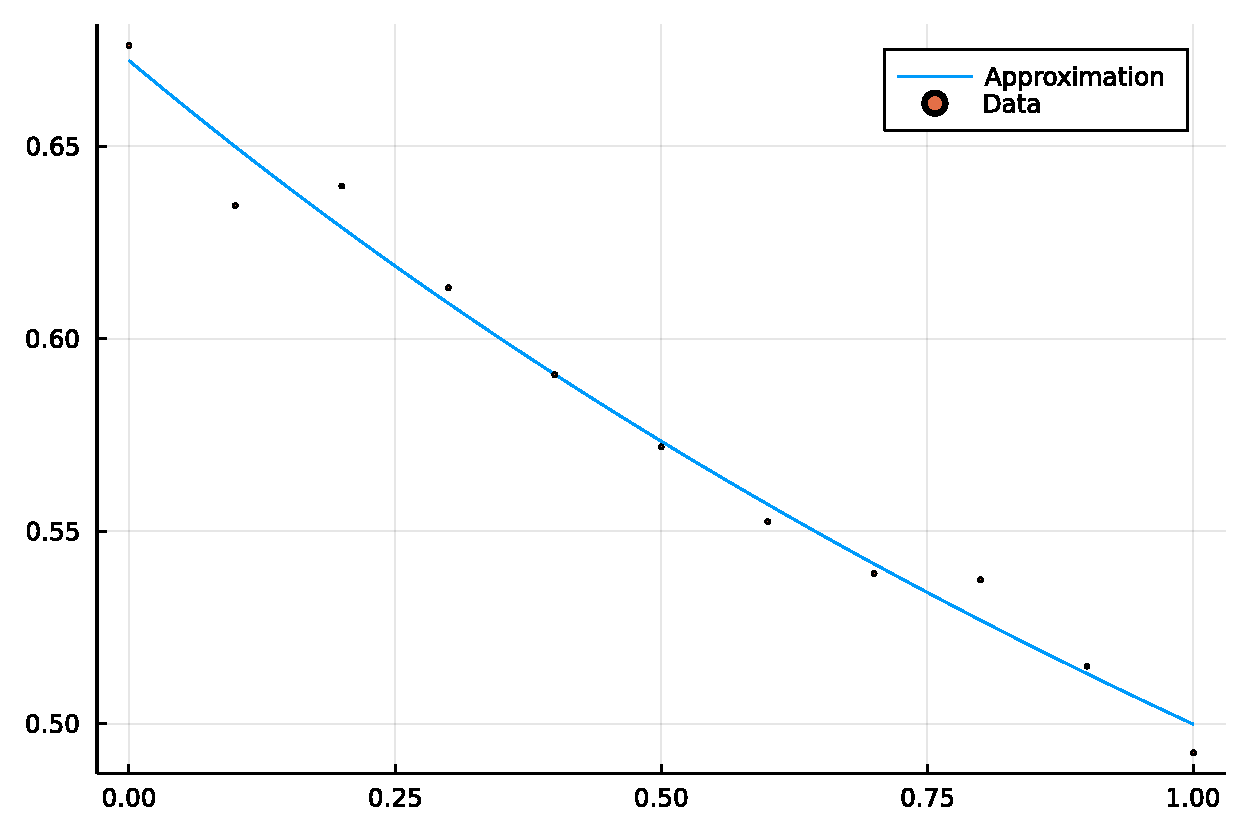
\includegraphics[width=0.6\linewidth]{figures/approx.pdf}
        \caption{Solution to \cref{exercise:nonlinear_approximation}.}%
        \label{fig:solution_exercise_approximation}
    \end{figure}
\end{exercise}

% \begin{exercise}
%     [Proof of convergence for Newton--Raphson]
%     The aim of this exercise is to prove the convergence of the Newton--Raphson method under simple assumptions.
%     Specifically, let $f \in C^2(\real)$ be a smooth function such that
%     \[
%         fa
%     \]
% \end{exercise}

\section{Discussion and bibliography}

The content of this chapter is largely based on the lecture notes~\cite{VanDooren}.
Several of the exercises are taken or inspired from~\cite{Legat}.
The proof of convergence of the secant method is inspired from the general proof presented in the short paper~\cite{MR1186462}.
For a detailed treatment of iterative methods for nonlinear equations,
see the book~\cite{MR1744713}.

\chapter{Numerical computation of eigenvalues}%
\label{cha:numerical_computation_of_eigenvalues}

Calculating the eigenvalues and eigenvectors of a matrix is a task often encountered in scientific and engineering applications.
Eigenvalue problems naturally arise in quantum physics,
solid mechanics, structural engineering and molecular dynamics,
to name just a few applications.
The aim of this chapter is to present an overview of the standard methods for calculating eigenvalues and eigenvectors numerically.

\chapter{Interpolation and approximation}%
\label{cha:interpolation_and_approximation}

\minitoc

\begin{figure}[ht]
    \centering
    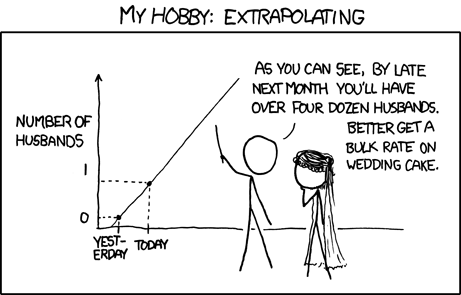
\includegraphics[width=0.5\linewidth]{figures/extrapolating.png}
\end{figure}

\section*{Introduction}
In this chapter,
we study numerical methods for interpolating and approximating functions.
The Cambridge dictionary defines interpolation as \emph{the addition of something different in the middle of a text, piece of music, etc.~or the thing that is added}.
The concept of interpolation in mathematics is consistent with this definition;
interpolation consists in finding, given a set of points~$(x_i, y_i)$,
a function~$f$ in a finite-dimensional space that goes through these points.
Throughout this course, you use the~\julia{plot} function in Julia,
which performs piecewise linear interpolation for drawing functions,
but there are a number of other standard interpolation methods.
Our first goal in this chapter is to present an overview of these methods and the associated error estimates.

In the second part of this chapter,
we focus of \emph{function approximation},
which is closely related to the subject of mathematical interpolation.
Indeed, a simple manner for approximating a general function by another one in a finite-dimensional space is to select a set of real numbers on the $x$ axis,
called \emph{nodes}, and find the associated interpolant.
As we shall demonstrate, not all sets of interpolation nodes are equal,
and special care is required in order to avoid undesired oscillations.
The field of function approximation is vast,
so our aim in this chapter is to present only an introduction to the subject.
In order to quantify the quality of an approximation,
a metric on the space of functions,
or a subset thereof, must be specified in order to measure errors.
Without a metric, saying that two functions are close is almost meaningless!
% Consider, for example, the function $f\colon [0, 1] \to \real; x \mapsto 0$ and the approximations $\widehat f_1(x) = x^{100}$ and $\widehat f_2(x) = 0.01$

\section{Interpolation}
Assume that we are given $n+1$ nodes $x_0, \dotsc, x_n$ on the $x$ axis,
together with values $u_0, \dotsc, u_n$,
which may be the values taken by an unknown function~$u(x)$ when evaluated at these points.
Suppose that we are looking for an interpolation~$\widehat u(x)$ in a subspace~$\Span \{\varphi_0, \dotsc, \varphi_n\}$
of the vector space of continuous functions, i.e.~an interpolating function of the form
\[
    \widehat u(x) = \alpha_0 \varphi_0(x) + \dotsb + \alpha_n \varphi_n(x),
\]
where $\alpha_0, \dotsc, \alpha_n$ are real coefficients.
In order for~$\widehat u(x)$ to be an interpolating function,
we must require that
\[
    \forall i \in \{0, \dotsc, n\}, \qquad
    \widehat u(x_i) = u_i.
\]
This leads to a linear system of $n+1$ equations and $n+1$ unknowns,
the latter being the coefficients~$\alpha_0, \dotsc, \alpha_n$.
This system of equations in matrix form reads
\begin{equation}
    \label{eq:linear_system_interpolation}
    \begin{pmatrix}
        \varphi_0(x_0) & \varphi_1(x_0) & \hdots & \varphi_n(x_0) \\
        \varphi_0(x_1) & \varphi_1(x_1) & \hdots & \varphi_n(x_1) \\
        \vdots & \vdots & & \vdots \\
        \varphi_0(x_n) & \varphi_1(x_n) & \hdots & \varphi_n(x_n)
    \end{pmatrix}
    \begin{pmatrix}
        \alpha_0 \\
        \alpha_1 \\
        \vdots \\
        \alpha_n
    \end{pmatrix}
    =
    \begin{pmatrix}
        u_0 \\
        u_1 \\
        \vdots \\
        u_n
    \end{pmatrix}.
\end{equation}

\subsection{Vandermonde matrix}
Since polynomials are very convenient for evaluation, integration, and differentiation,
they are a natural choice for interpolation purposes.
The simplest basis of the subspace of polynomials of degree less than or equal to $n$ is given by the monomials:
\[
    \varphi_0(x) = 1,
    \qquad
    \varphi_1(x) = x,
    \qquad \dotsc, \qquad
    \varphi_n(x) = x^n.
\]
In this case,
the linear system~\eqref{eq:linear_system_interpolation} for determining the coefficients of the interpolant reads
\begin{equation}
    \label{eq:linear_system_interpolation_poly}
    \begin{pmatrix}
        1 & x_0 & \hdots & x_0^n \\
        1 & x_1 & \hdots & x_1^n \\
        \vdots & \vdots & & \vdots \\
        1 & x_n & \hdots & x_n^n
    \end{pmatrix}
    \begin{pmatrix}
        \alpha_0 \\
        \alpha_1 \\
        \vdots \\
        \alpha_n
    \end{pmatrix}
    =
    \begin{pmatrix}
        u_0 \\
        u_1 \\
        \vdots \\
        u_n
    \end{pmatrix}.
\end{equation}
The matrix on the left-hand side is called a \emph{Vandermonde} matrix.
If the abcissae $x_0, \dotsc, x_n$ are distinct,
then this is a full rank matrix,
and so~\eqref{eq:linear_system_interpolation_poly} admits a unique solution,
implying as a corollary that the interpolating polynomial exists and is unique.
It is possible to show that the condition number of the Vandermonde increases dramatically with $n$.
Consequently, solving~\eqref{eq:linear_system_interpolation_poly} is not a viable method in practice for calculating the interpolating polynomial.

\subsection{Lagrange interpolation formula}
One may wonder whether polynomial basis functions $\varphi_0, \dotsc, \varphi_n$ can be defined in such a manner that
the matrix in~\eqref{eq:linear_system_interpolation} is the identity matrix.
The answer to this question is positive;
it suffices to take as a basis the \emph{Lagrange polynomials},
which are given by
\[
    \varphi_{i}(x)
    = \frac{(x - x_0) (x - x_1) \dotsc (x - x_{i-1}) (x - x_{i+1}) \dotsc (x - x_n)}
    {(x_i - x_0) (x_i - x_1) \dotsc (x_i - x_{i-1}) (x_i - x_{i+1}) \dotsc (x_i - x_n)}.
\]
It is simple to check that
\[
    \varphi_i(x_j) =
    \delta_{i,j} =
    \begin{cases}
        1 & \text{if $i = j$}, \\
        0 & \text{otherwise.}
    \end{cases}
\]
Finding the interpolant in this basis is immediate:
\[
    \widehat u(x) = u_1 \varphi_1(x) + \dotsb + u_n \varphi_n(x).
\]
While simple, this approach to polynomial interpolation has a few disadvantages:
\begin{itemize}
    \item
        First, evaluating $\widehat u(x)$ is computationally costly when $n$ is large.

    \item
        Second, all the basis functions change when adding new interpolation nodes.

    \item
        Finally, Lagrange interpolation is numerically unstable because of cancellations between large terms.
        Indeed, it is often the case that Lagrange polynomials take very large values over the interpolation intervals;
        this occurs, for example,
        when many equidistant interpolation nodes are employed,
        as illustrated in~\cref{fig:lagrange}.
\end{itemize}
\begin{figure}[ht]
    \centering
    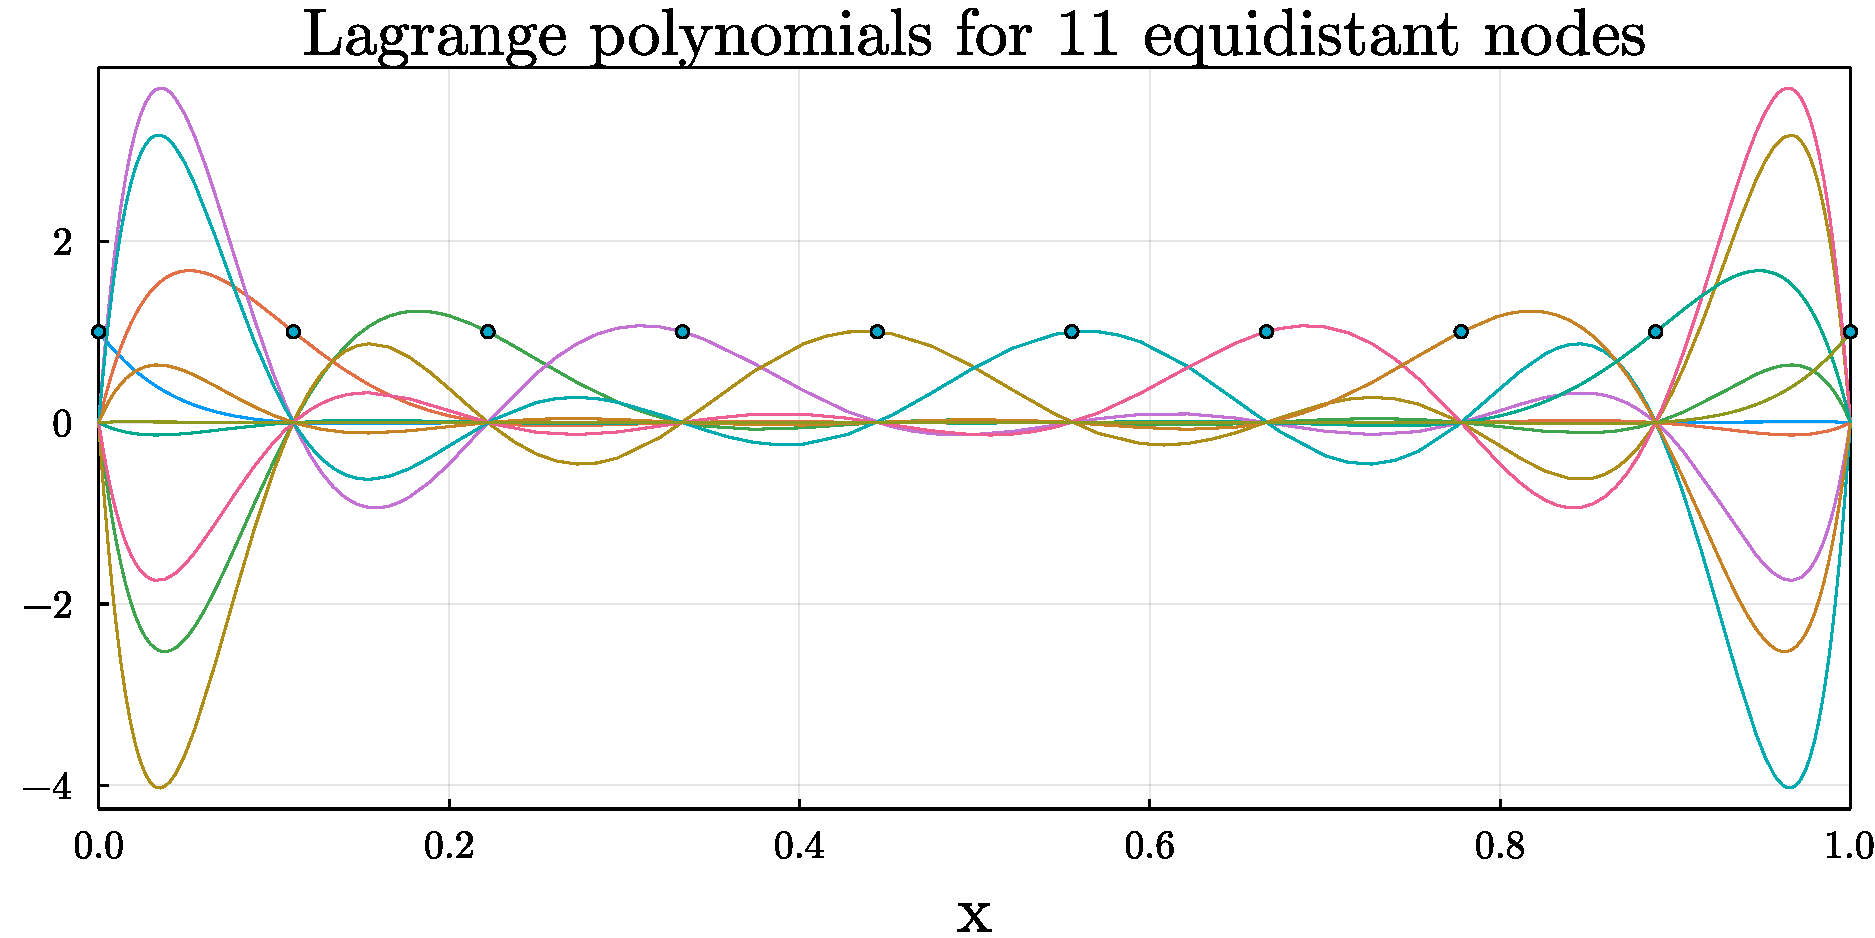
\includegraphics[width=0.8\linewidth]{figures/lagrange_10.pdf}
    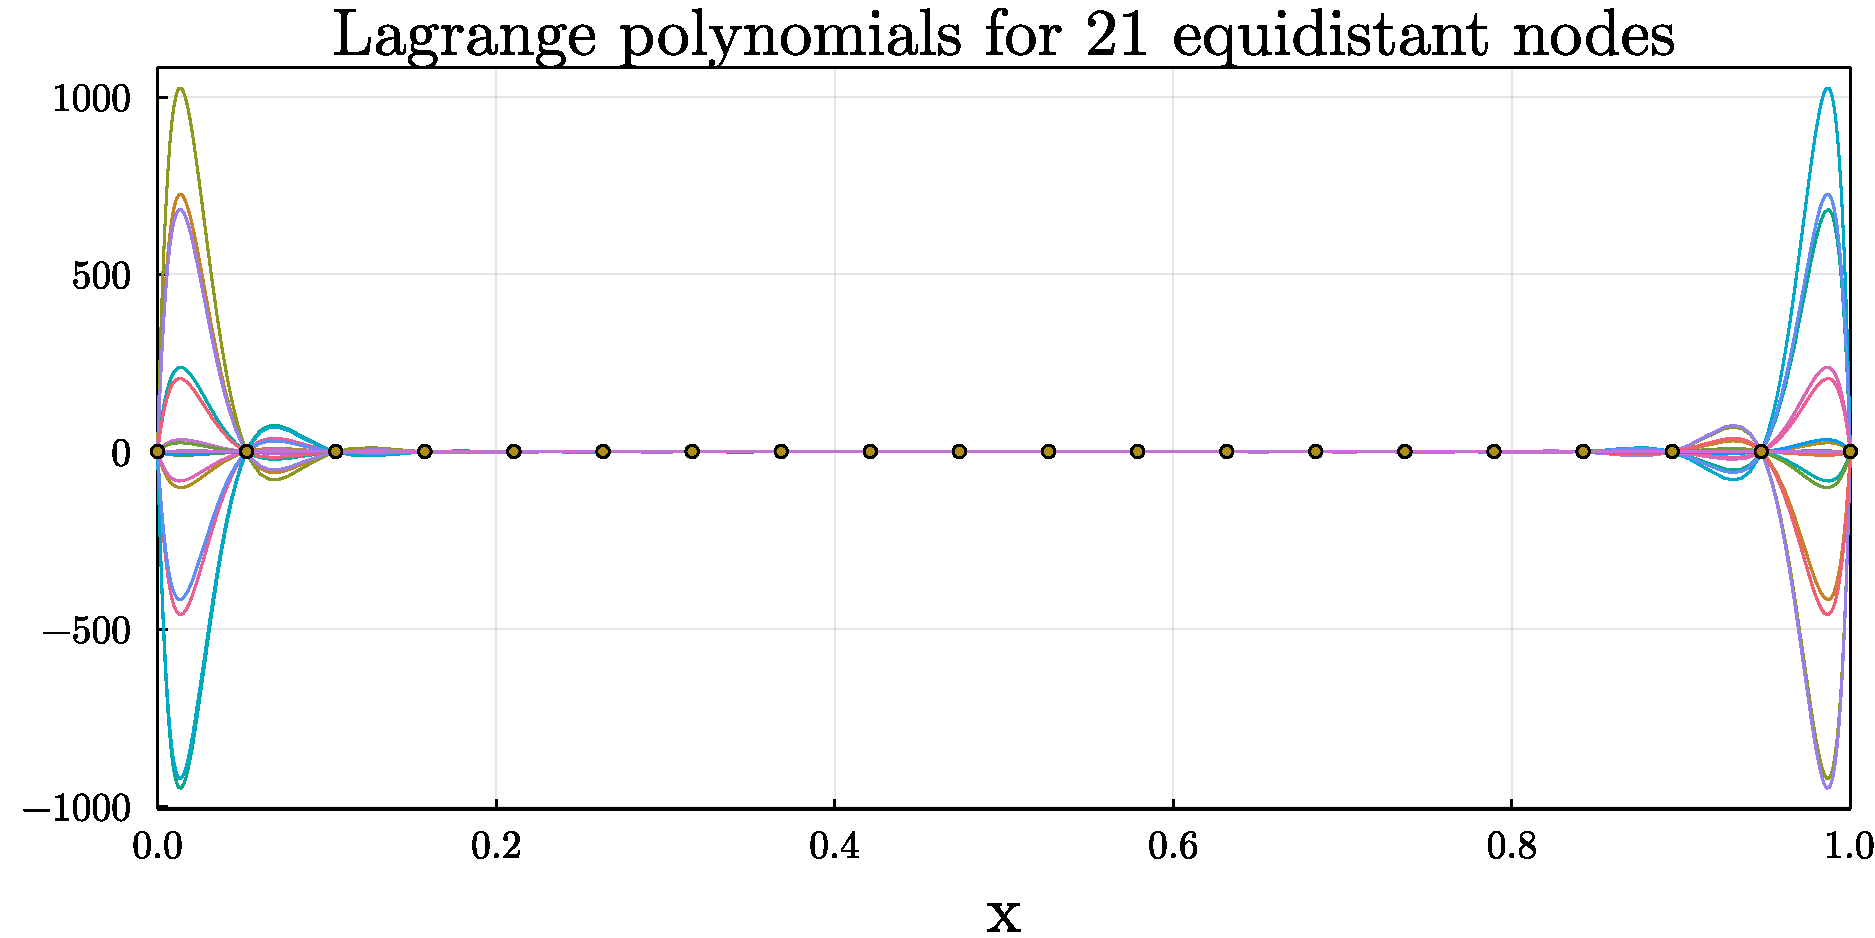
\includegraphics[width=0.8\linewidth]{figures/lagrange_20.pdf}
    \caption{Lagrange polynomials associated with equidistant nodes over the $(0, 1)$ interval.}%
    \label{fig:lagrange}
\end{figure}

\subsection{Gregory--Newton interpolation}
By Taylor's formula,
any polynomial~$p$ of degree $n$ may be expressed as
\begin{equation}
    \label{eq:taylor}
    p(x) = p(0) + p'(0) x + \frac{p''(0)}{2} x^2 + \dotsc + \frac{p^{(n)}(0)}{n!} x^n.
\end{equation}
The constant coefficient can be obtained by evaluating the polynomial at 0,
the linear coefficient can be identified by evaluating the first derivative at 0,
and so on.
Assume now that we are given the values taken by~$p$ when evaluated at the integer numbers $\{0, \dotsc, n\}$.
We ask the following question:
can we find a formula similar in spirit to~\eqref{eq:taylor},
but including only evaluations of $p$ and not of its derivatives?
To answer this question, we introduce the difference operator $\Delta$ which acts on functions as follows:
\[
    \Delta f(x) = f(x+1) - f(x).
    % (p_0, p_1, \dotsc) \mapsto (p_1 - p_0, p_2 - p_1, \dotsc).
\]
The operator~$\Delta$ is a linear operator on the space of continuous functions.
It maps constant functions to 0,
and the linear function~$x$ to the constant function~$1$,
suggesting a resemblance with the differentiation operator.
In order to further understand this connection,
let us define the \emph{falling power} of a real number $x$ as
\[
    x^{\underline{k}} = x (x-1) (x-2) \dots (x-k+1).
\]
We then have that
\begin{align}
    \nonumber
    \Delta x^{\underline{k}}
    &= (x+1) x (x-1) \dots (x-k+2) - x (x-1) (x-2) \dots (x-k+1) \\
    \label{eq:falling_powers_rule}
    &= \bigl((x+1) - (x-k+1)\bigr) \bigl(x (x-1) \dots (x-k+2)\bigr) = k x^{\underline{k-1}}
\end{align}
In other words,
the action of the difference operator on falling powers mirrors that of the differentiation operator on monomials.
The falling powers form a basis of the space of polynomials,
and so any polynomial in~$\poly(n)$, i.e.\ of degree less than or equal to $n$, can be expressed as
\begin{equation}
    \label{eq:gregory_newton}
    p(x) = \alpha_0 + \alpha_1 x^{\underline{1}} + \alpha_2 x^{\underline{2}} + \dotsb + \alpha_n x^{\underline{n}}.
\end{equation}
It is immediate to show that $\alpha_i = \Delta^i p(0)$,
where $\Delta^i p$ denotes the function obtained after~$i$ applications of the operator~$\Delta$.
Therefore, any polynomial of degree less than or equal to~$n$ may be expressed as
\begin{equation}
    \label{eq:gregory_newton_actually}
    p(x) = p(0) + \Delta p(0) x^{\underline{1}} + \frac{\Delta^2 p(0)}{2} x^{\underline{2}} + \dotsb + \frac{\Delta^n p(0)}{n!} x^{\underline{n}}.
\end{equation}
An expansion of the form~\eqref{eq:gregory_newton_actually} is called a \emph{Newton series},
which is the discrete analog of the continuous Taylor series.
From the definition of~$\Delta$,
it is clear that the coefficients in~\eqref{eq:gregory_newton_actually} depend only on~$p(0), \dotsc, p(n)$.
We conclude that, given points $n+1$ points $(i, u_i)$ for $i \in \{0, \dotsc, n\}$,
the unique interpolating polynomial is given by~\eqref{eq:gregory_newton_actually},
after replacing $p(i)$ by $u_i$.

\begin{example}
    \label{example:gregory_newton}
    Let us use~\eqref{eq:gregory_newton} in order to calculate the value of
    \[
        S(n) := \sum_{i=0}^{n} i^2.
    \]
    Since $\Delta S(n) = (n+1)^2$,
    which is a second degree polynomial in $n$,
    we deduce that $S(n)$ is a polynomial of degree 3.
    % Notice the slight abuse of notation here:
    % since $S(n)$ is well-defined only for $n \in \nat$,
    % $\Delta S(n)$ is also well-defined
    Let us now determine its coefficients.
    \begin{center}
    \begin{tabular}{|c|c|c|c|c|}
        \hline
        $n$    & $0$ & $1$ & $2$ & $3$ \\ \hline
        $\Delta^0 S(n)$ & $\mathbf{0}$ & $1$ & $5$ & $14$ \\ \hline
        $\Delta^1 S(n)$ & $\mathbf{1}$ & $4$ & $9$ &  \\ \hline
        $\Delta^2 S(n)$ & $\mathbf{3}$ & $5$ & & \\ \hline
        $\Delta^3 S(n)$ & $\mathbf{2}$ & & & \\ \hline
    \end{tabular}
    \end{center}
    We conclude that
    \[
        S(n) = \mathbf{1} n + \frac{\mathbf{3}}{2!} n(n-1) + \frac{\mathbf{2}}{3!} n(n-1)(n-2)
        = \frac{n (2n+1) (n+1)}{6}
    \]
\end{example}
Notice that when falling powers are employed as polynomial basis,
the matrix in~\eqref{eq:linear_system_interpolation} is lower triangular,
and so the algorithm described in~\cref{example:gregory_newton} could be replaced by the forward substitution method.
Whereas the coefficients of the Lagrange interpolant can be obtained immediately from the values of~$u$ at the nodes,
calculating the coefficients of the expansion in~\eqref{eq:gregory_newton} requires $\mathcal O(n^2)$ operations.
However, Gregory--Newton interpolation has several advantages over Lagrange interpolation:
\begin{itemize}
    \item
        If a point~$(n+1, p_{n+1})$ is added to the set of interpolation points,
        only one additional term, corresponding to the falling power~$x^{\underline{n+1}}$,
        needs to be calculated in~\eqref{eq:gregory_newton_actually}.
        All the other coefficients are unchanged.
        Therefore, the Gregory--Newton approach is well-suited for incremental interpolation.

    \item
        The Gregory--Newton interpolation method is more numerically stable than Lagrange interpolation,
        because the basis functions do not take very large values.

    \item
        A polynomial in the form of a Newton series can be evaluated efficiently using Horner's method,
        which is based on rewriting the polynomial as
        \[
            p(x) = \alpha_0 + x \biggl( \alpha_1 + (x-1)  \Bigl( \alpha_2 + (x-2)\bigl(\alpha_3 + (x-3) \dotsc \bigr) \Bigr)  \biggr).
        \]
        Evaluating this expression starting from the innermost bracket leads to an algorithm with a cost scaling linearly with the degree of the polynomial.
\end{itemize}

\subsubsection*{Non-equidistant nodes}%
So far,
we have described the Gregory--Newton method in the simple setting where interpolation nodes are just a sequence of successive natural numbers.
The method can be generalized to the setting of nodes $x_0 \neq \dotsc \neq x_n$ which are not necessarily equidistant.
In this case, we take as basis the following functions instead of the falling powers:
\begin{equation}
    \label{eq:basis_newton}
    \varphi_{i}(x) = (x - x_0) (x - x_1) \dotsc (x - x_{i-1}),
\end{equation}
with the convention that the empty product is 1.
By~\eqref{eq:linear_system_interpolation},
the coefficients of the interpolating polynomial in this basis solve the following linear system:
\begin{equation}
    \label{eq:matrix_newton}
    \begin{pmatrix}
        1 &         & \ldots &        & 0  \\
        1 & x_1-x_0 &        &        &    \\
        1 & x_2-x_0 & (x_2-x_0)(x_2-x_1) &        & \vdots   \\
        \vdots & \vdots  &        & \ddots &    \\
        1 & x_n-x_0 & \ldots & \ldots & \prod_{j=0}^{n-1}(x_n - x_j)
    \end{pmatrix}
    \begin{pmatrix}
        \alpha_0 \\
        \alpha_1 \\
        \alpha_2 \\
        \vdots \\
        \alpha_n
    \end{pmatrix}
    =
    \begin{pmatrix}
        u_0 \\
        u_1 \\
        u_2 \\
        \vdots \\
        u_n
    \end{pmatrix}.
\end{equation}
This system could be solved using, for example, forward substitution.
Clearly $\alpha_0 = u_0$ from the first equation,
and then from the second equation we obtain
\[
    \alpha_1 = \frac{u_1 - u_0}{x_1 - x_0} =: [u_0, u_1],
\]
which may be viewed as an approximation of the slope of~$u$ at $x_0$.
The right-hand side of this equation is an example of a \emph{divided difference}.
In general, divided differences are defined recursively as follows:
\begin{equation}
    \label{eq:definition_divided_difference}
    [u_{0}, u_{2}, \dotsc, u_{d}] := \frac{[u_{1}, \dotsc, u_{d}] - [u_{0}, \dotsc, u_{d-1}]}{x_{d}-x_{0}}, \qquad [u_i] = u_i.
\end{equation}
It is possible to find an expression for the coefficients of the interpolating polynomials in terms of these divided differences.
\begin{proposition}
    Assume that $(x_0, u_0), \dotsc, (x_n, u_n)$ are $n+1$ points in the plane with distinct abcissae.
    Then the interpolating polynomial of degree $n$ may be expressed as
    \[
        p(x) = \sum_{i=0}^{n} [u_0, \dotsc, u_n] \varphi_i(x),
    \]
    where $\varphi_i(x)$, for $i = 0, \dotsc, n$, are the basis functions defined in~\eqref{eq:basis_newton}.
\end{proposition}
\begin{proof}
    The statement is true for $n = 0$.
    Reasoning by induction, we assume that it holds true for polynomials of degree up to $n-1$.
    Let $p_1(x)$ and $p_2(x)$ be the interpolating polynomials at the points
    $x_0, x_1, \dotsc, x_{n-2}, x_{n-1}$ and $x_0, x_1, \dotsc, x_{n-2}, x_{n}$, respectively.
    Then
    \begin{equation}
        \label{eq:interpolating_polynomial}
        p(x) = p_1(x) + \frac{x - x_{n-1}}{x_n - x_{n-1}} \bigl(p_2(x) - p_1(x)\bigr)
    \end{equation}
    is a polynomial of degree~$n$ that interpolates all the data points.
    By the induction hypothesis,
    it holds that
    \begin{align*}
        p_1(x) &= u_0 + [u_0, u_1] (x - x_0) + \dotsc + [u_0, u_1, \dotsc, u_{n-2}, \mathbf{u_{n-1}}] \prod_{i=0}^{n-2} (x - x_i), \\
        p_2(x) &= u_0 + [u_0, u_1] (x - x_0) + \dotsc + [u_0, u_1, \dotsc, u_{n-2}, \mathbf{u_{n}}] \prod_{i=0}^{n-2} (x - x_i).
    \end{align*}
    Here we used a bold font in order to emphasize the difference between the two expressions.
    Substituting these expressions in~\eqref{eq:interpolating_polynomial},
    we obtain
    \begin{align*}
        p(x) =
        &u_0 + [u_0, u_1] (x - x_0) + \dotsc + [u_0, \dotsc, u_{n-2}] \prod_{i=0}^{n-2} (x - x_i)  \\
        & + \frac{[u_0, u_1, \dotsc, u_{n-2}, u_{n-1}] - [u_0, u_1, \dotsc, u_{n-2}, u_{n}]}{x_n - x_{n-1}} \prod_{i=0}^{n-1} (x - x_i).
    \end{align*}
    In \cref{exercise:divided_differences},
    we show that divided differences are invariant under permutations of the data points,
    and so we have that
    \[
        \frac{[u_0, u_1, \dotsc, u_{n-2}, u_{n-1}] - [u_0, u_1, \dotsc, u_{n-2}, u_{n}]}{x_n - x_{n-1}} = [u_0, \dotsc, u_n],
    \]
    which enables to conclude.
\end{proof}
\begin{example}
    Assume that we are looking for the third degree polynomial going through the following points:
    \[
        (-1, 10), \qquad (0, 4), \qquad (2, -2), \qquad (4, -40).
    \]
    We have to calculate the divided difference $\alpha_i = [u_0, \dotsc, u_i]$ for $i \in \{0, 1, 2, 3\}$.
    To this end,
    it is convenient to use a table:
    \begin{center}
    \begin{tabular}{|c|c|c|c|c|}
        \hline
        $i$ & $0$ & $1$ & $2$ & $3$ \\ \hline
        $[u_i]$ & $\mathbf{10}$ & $4$ & $-2$ & $-40$ \\ \hline
        $x_{i+1} - x_{i}$ & $1$ & $2$ & $2$ &  \\ \hline
        $[u_i, u_{i+1}]$ & $\mathbf{-6}$ & $-3$ & $-19$ &  \\ \hline
        $x_{i+2} - x_{i}$ & $3$ & $4$ &  &  \\ \hline
        $[u_i, u_{i+1}, u_{i+2}]$ & $\mathbf{1}$ & $-4$ & & \\ \hline
        $x_{i+3} - x_{i}$ & $5$  & &  &  \\ \hline
        $[u_i, u_{i+1}, u_{i+2}, u_{i+3}]$ & $\mathbf{-1}$ & & & \\ \hline
    \end{tabular}
    \end{center}
    We deduce that the expression of the interpolating polynomial is
    \[
        p(x)
        = \mathbf{10} + (\mathbf{-6})(x+1) + \mathbf{1} (x+1)x + (\mathbf{-1}) (x+1)x(x-2)
        = - x^3 + 2 x^2 + -3x + 4.
    \]
\end{example}

\subsection{Interpolation error}
Assume that~$u(x)$ is a continuous function and denote by $\widehat u(x)$ its interpolation through the points~$(x_i, u_i)$,
where $u_i = u(x_i)$ for $i = 0, \dotsc, n$.
In this section, we study the behavior of the error in the limit as $n \to \infty$.

\begin{theorem}
    [Interpolation error]
    \label{theorem:interpolation_error}
    Assume that~$u\colon [a, b] \to \real$ is a function in $C^{n+1}([a, b])$ and let~$x_0, \dotsc, x_n$ denote $n+1$ distinct interpolation nodes.
    Then for all $x \in [a, b]$,
    there exists~$\xi = \xi(x)$ in the interval $[a, b]$ such that
    \[
        e_n(x) := u(x) - \widehat u(x) = \frac{u^{(n+1)}(\xi)}{(n+1)!} (x-x_0) \dotsc (x - x_n).
    \]
\end{theorem}
\begin{proof}
    The statement is obvious if $x \in \{x_0, \dotsc, x_n\}$,
    so we assume from now on that $x$ does not coincide with an interpolation node.
    Let us use the compact notation $\omega_n = \prod_{i=0}^n (x - x_i)$ and introduce the function
    \begin{equation}
        \label{eq:interpolation_error}
        g(t) = e_n(t) \omega_n(x) - e_n(x) \omega_n(t).
    \end{equation}
    The function $g$ is smooth and takes the value~0 when evaluated at~$x_0, \dotsc, x_n, x$.
    Since $g$ has $n+2$ roots in the interval $[a, b]$,
    Rolle's theorem implies that $g'$ has at least $n+1$ distinct roots in~$(a, b)$.
    Another application of Rolle's theorem then yields that $g''$ has at least $n$ distinct roots in~$(a, b)$.
    Iterating this reasoning, we deduce that $g^{(n+1)}$ has one root~$t_*$ in $(a, b)$.
    From~\eqref{eq:interpolation_error},
    we calculate that
    \begin{equation}
        \label{eq:interpolation_error_proof}
        g^{(n+1)}(t) = e_n^{(n+1)}(t) \omega_n(x) - e_n(x) \omega_n^{(n+1)}(t)
        = u^{(n+1)}(t) \omega_n(x) - e_n(x) (n+1)!.
    \end{equation}
    Here we employed the fact that $\widehat u^{(n+1)}(t) = 0$,
    because $\widehat u$ is a polynomial of degree at most $n$.
    Evaluating~\eqref{eq:interpolation_error_proof} at~$t_*$ and rearranging,
    we obtain that
    \[
        e_n(x) = \frac{u^{(n+1)}(t_*)}{(n+1)!} \omega_n(x),
    \]
    which completes the proof.
\end{proof}
As a corollary to~\cref{theorem:interpolation_error},
we deduce the following error bound.
\begin{corollary}
    [Upper bound on the interpolation error]
    \label{corollary:interpolation_error}
    Assume that $u$ is smooth in the interval $[a, b]$ and let
    \[
        C_{n+1} =
        \sup_{x \in [a, b]} \left\lvert u^{(n+1)}(x) \right\rvert.
    \]
    Then
    \begin{equation}
        \label{eq:upper_bound_interp_error}
        E_n := \sup_{x \in [a, b]} \bigl\lvert e_n(x) \bigr\rvert \leq \frac{C_{n+1}}{4(n+1)} h^{n+1}
    \end{equation}
    where $h$ is the maximum spacing between two successive interpolation nodes.
\end{corollary}
\begin{proof}
By~\cref{theorem:interpolation_error},
it holds that
\begin{equation}
    \label{eq:bound_error_from_theorem}
    \forall x \in [a, b], \qquad
    \abs{e_n(x)} \leq \frac{C_{n+1}}{(n+1)!} \Bigl\lvert (x-x_0) \dotsc (x-x_n) \Bigr\rvert.
\end{equation}
The product on the right-hand side is bounded from above by
\begin{equation}
    \label{eq:interpolation_bound_product}
    \frac{h^2}{4} \times 2h \times 3h \times 4h \times \dotsb \times nh = \frac{n! h^{n+1}}{4}.
\end{equation}
The first factor comes from the fact that, if $x \in [x_i, x_{i+1}]$,
then
\[
    \Bigl\lvert (x - x_i)(x - x_{i+1}) \Bigr\rvert \leq \frac{(x_{i+1} - x_i)^2}{4},
\]
because the left-hand side is maximized when $x$ is the midpoint of the interval~$[x_i, x_{i+1}]$.
Substituting~\eqref{eq:interpolation_bound_product} into~\eqref{eq:bound_error_from_theorem},
we deduce the statement.
\end{proof}
We now ask the following natural question:
does $E_n$ given in~\eqref{eq:upper_bound_interp_error} tend to zero as the maximum spacing between successive nodes tends to 0?
By~\cref{corollary:interpolation_error},
the answer to this question is positive when $C_{n}$ does not grow too quickly as $n \to \infty$.
For example
the interpolation error for the function $u(x) = \sin(x)$
decreases very quickly as $n \to \infty$
when equidistant interpolation nodes are employed,
as illustrated in \cref{fig:interpolation_sine}.
\begin{figure}[ht!]
    \centering
    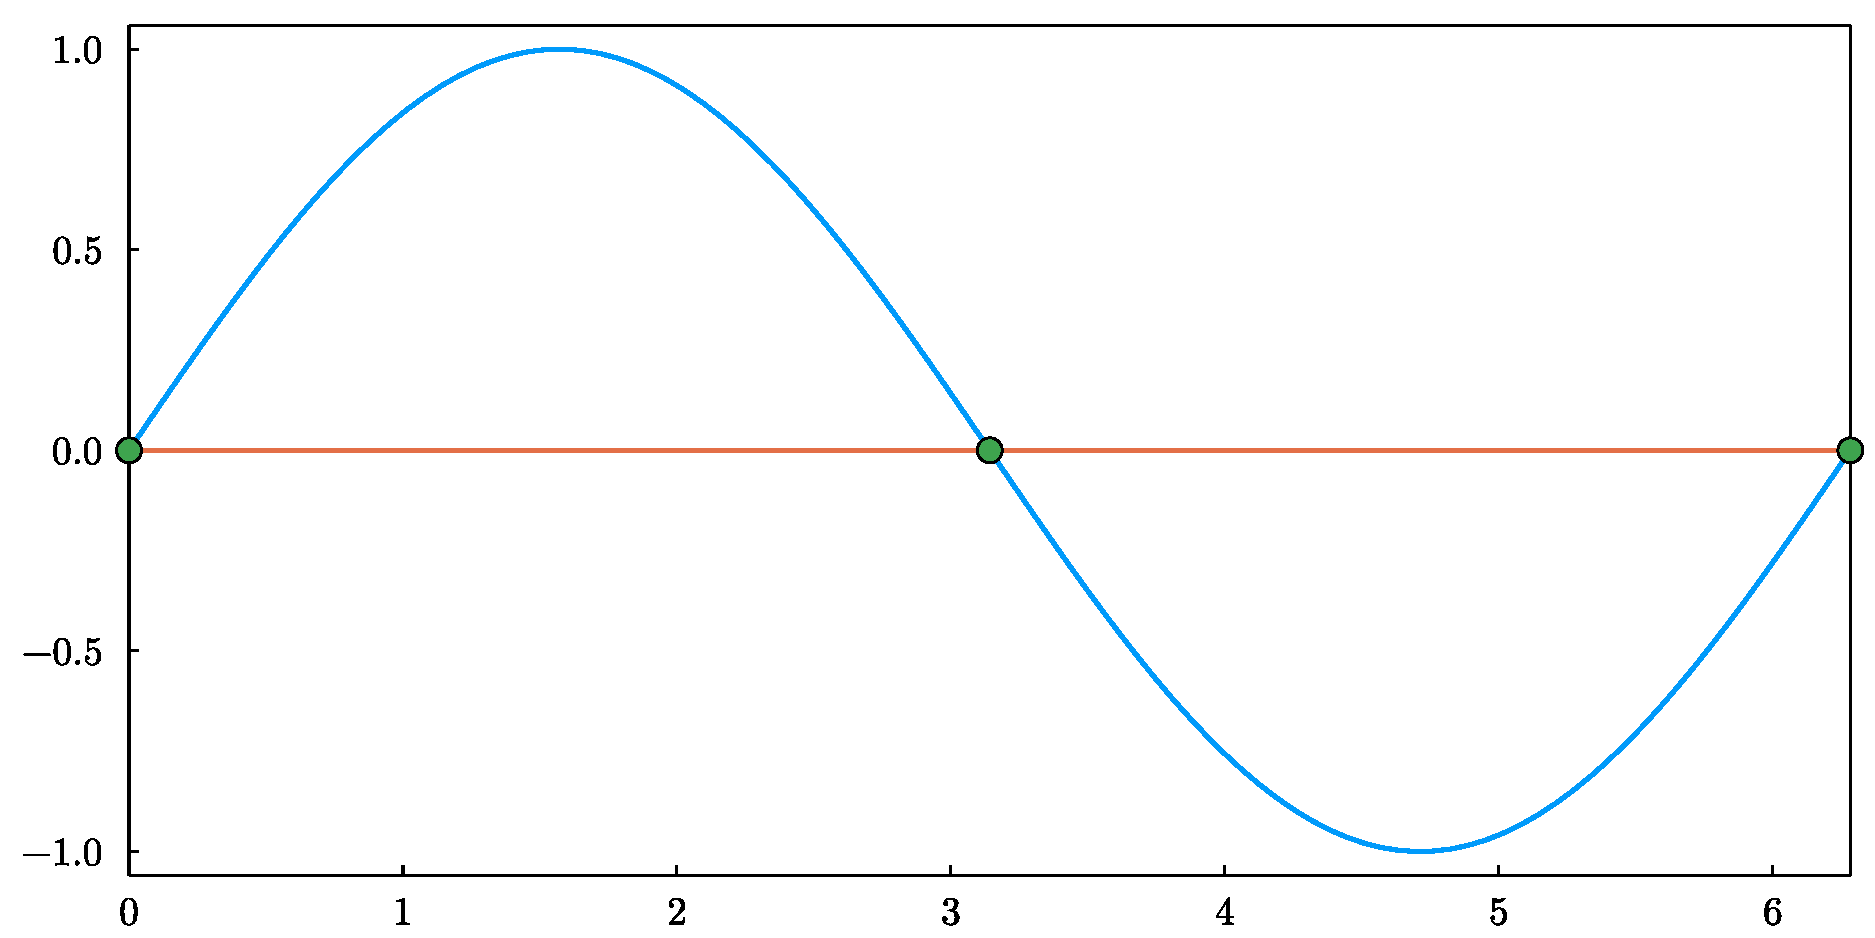
\includegraphics[width=0.49\linewidth]{figures/interpolation_sine_3.pdf}
    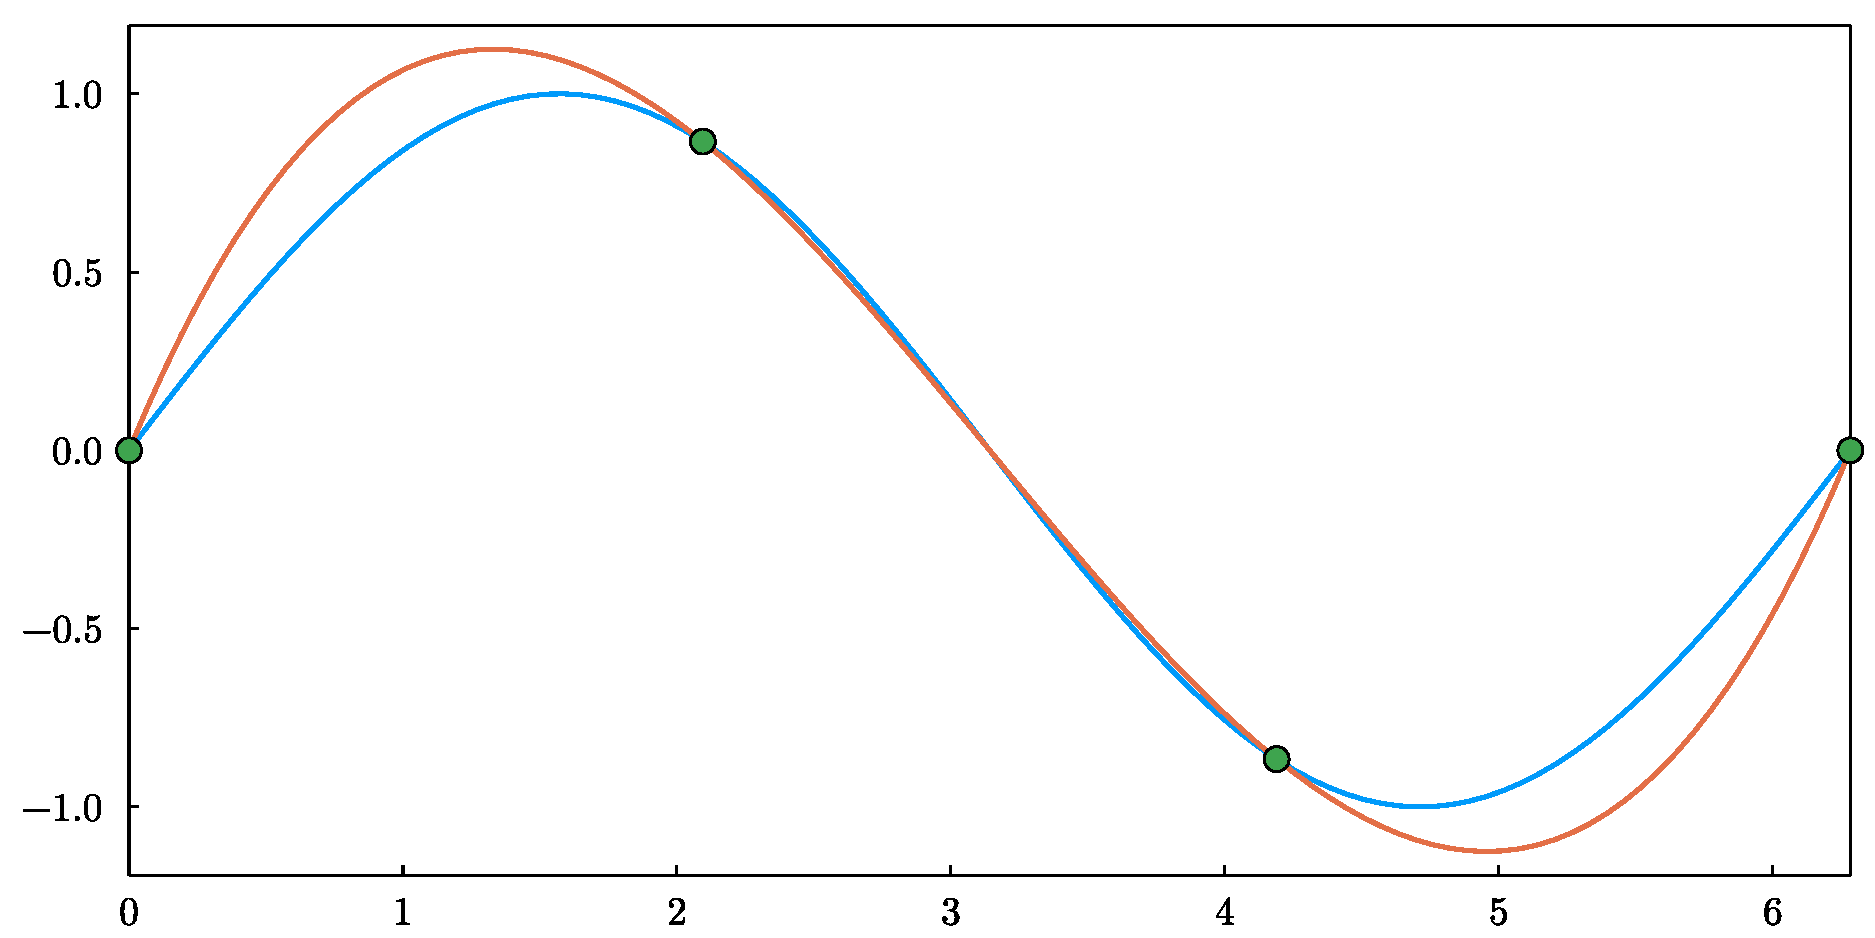
\includegraphics[width=0.49\linewidth]{figures/interpolation_sine_4.pdf}
    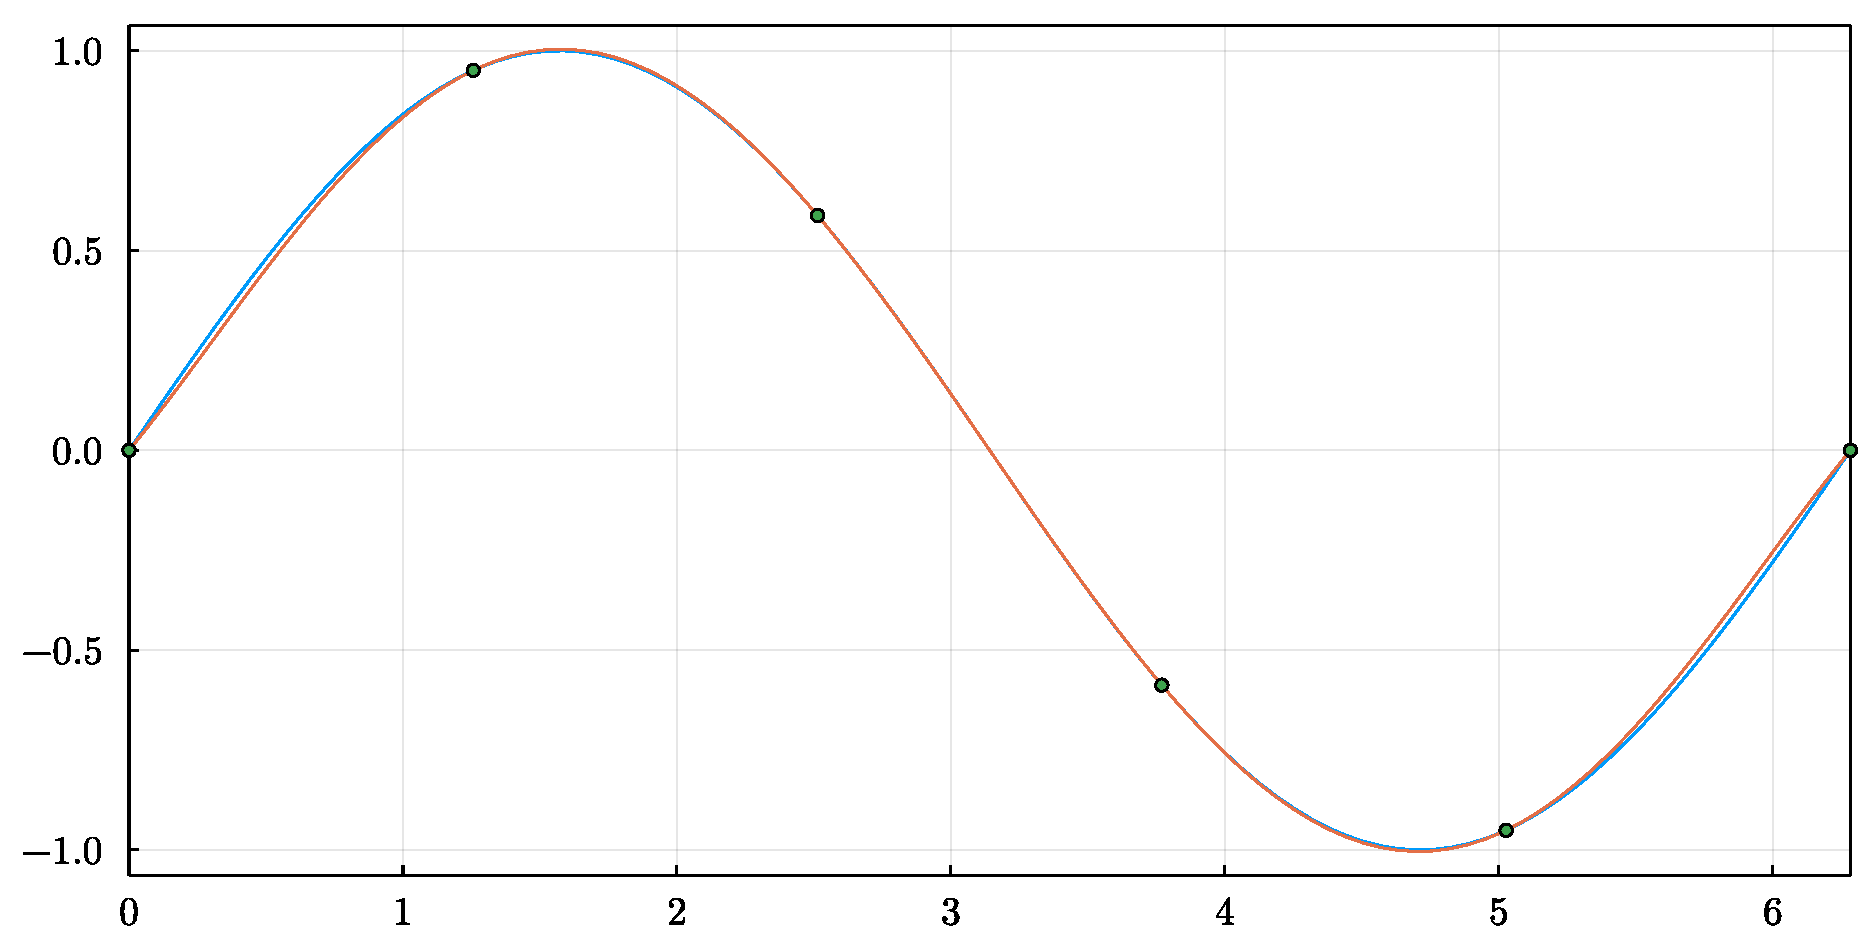
\includegraphics[width=0.49\linewidth]{figures/interpolation_sine_6.pdf}
    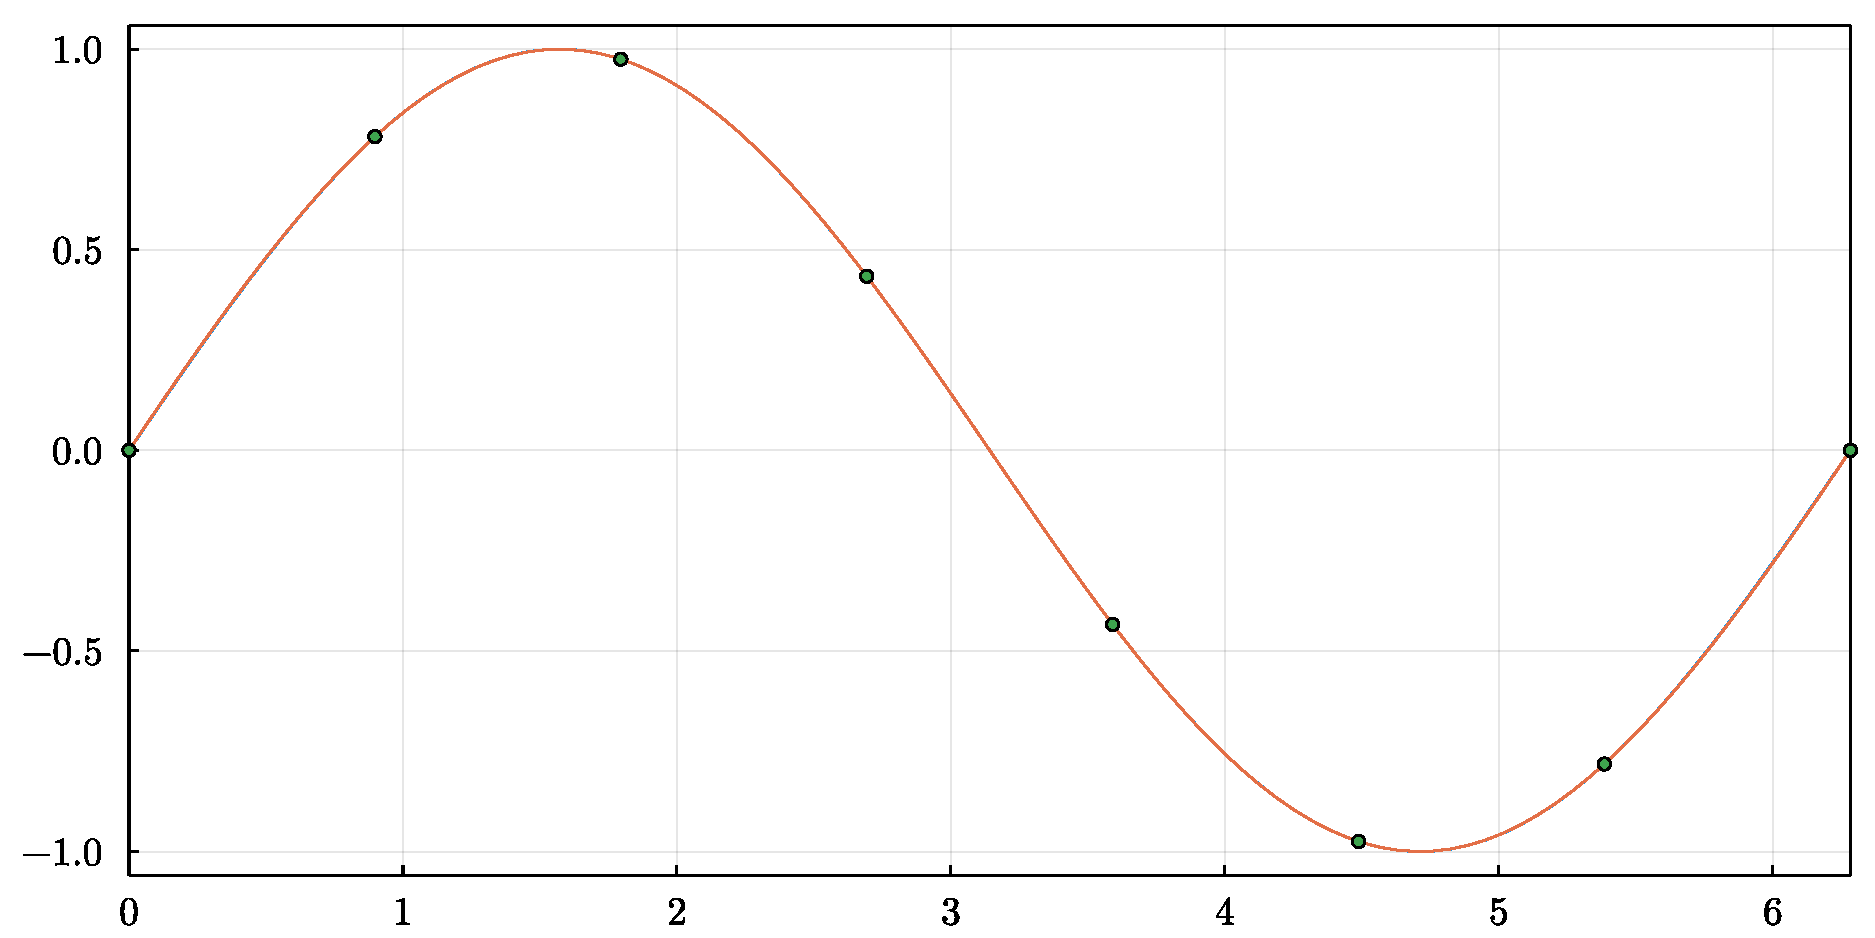
\includegraphics[width=0.49\linewidth]{figures/interpolation_sine_8.pdf}
    \caption{Interpolation (in orange) of the function $u(x) = \sin(x)$ (in blue) using 3, 4, 6, and 8 equidistant nodes.}%
    \label{fig:interpolation_sine}
\end{figure}

In some cases, however,
the constant $C_n$ grows quickly with $n$,
to the extent that $E_n$ may increase with $n$;
in this case, the maximum interpolation error grows when nodes are added!
The classic example illustrating this potential issue is that of the Runge function:
\begin{equation}
    \label{eq:runge_function}
    u(x) = \frac{1}{1 + 25 x^2}.
\end{equation}
It is possible to show that,
for this function,
the upper bound in~\eqref{eq:upper_bound_interp_error} tends to $\infty$ in the limit as the number~$n$ of interpolation nodes increases.
We emphasize that this does not prove that~$E_n \to \infty$ in the limit as $n \to \infty$,
because~\eqref{eq:upper_bound_interp_error} provides only an \emph{upper bound} on the error.
In fact, the interpolation error for the Runge function can either grow or decrease,
depending on the choice of interpolation nodes.
With equidistant nodes, it turns out that $E_n \to \infty$,
as illustrated in~\cref{fig:interpolation_runge_function}.
\begin{figure}[ht!]
    \centering
    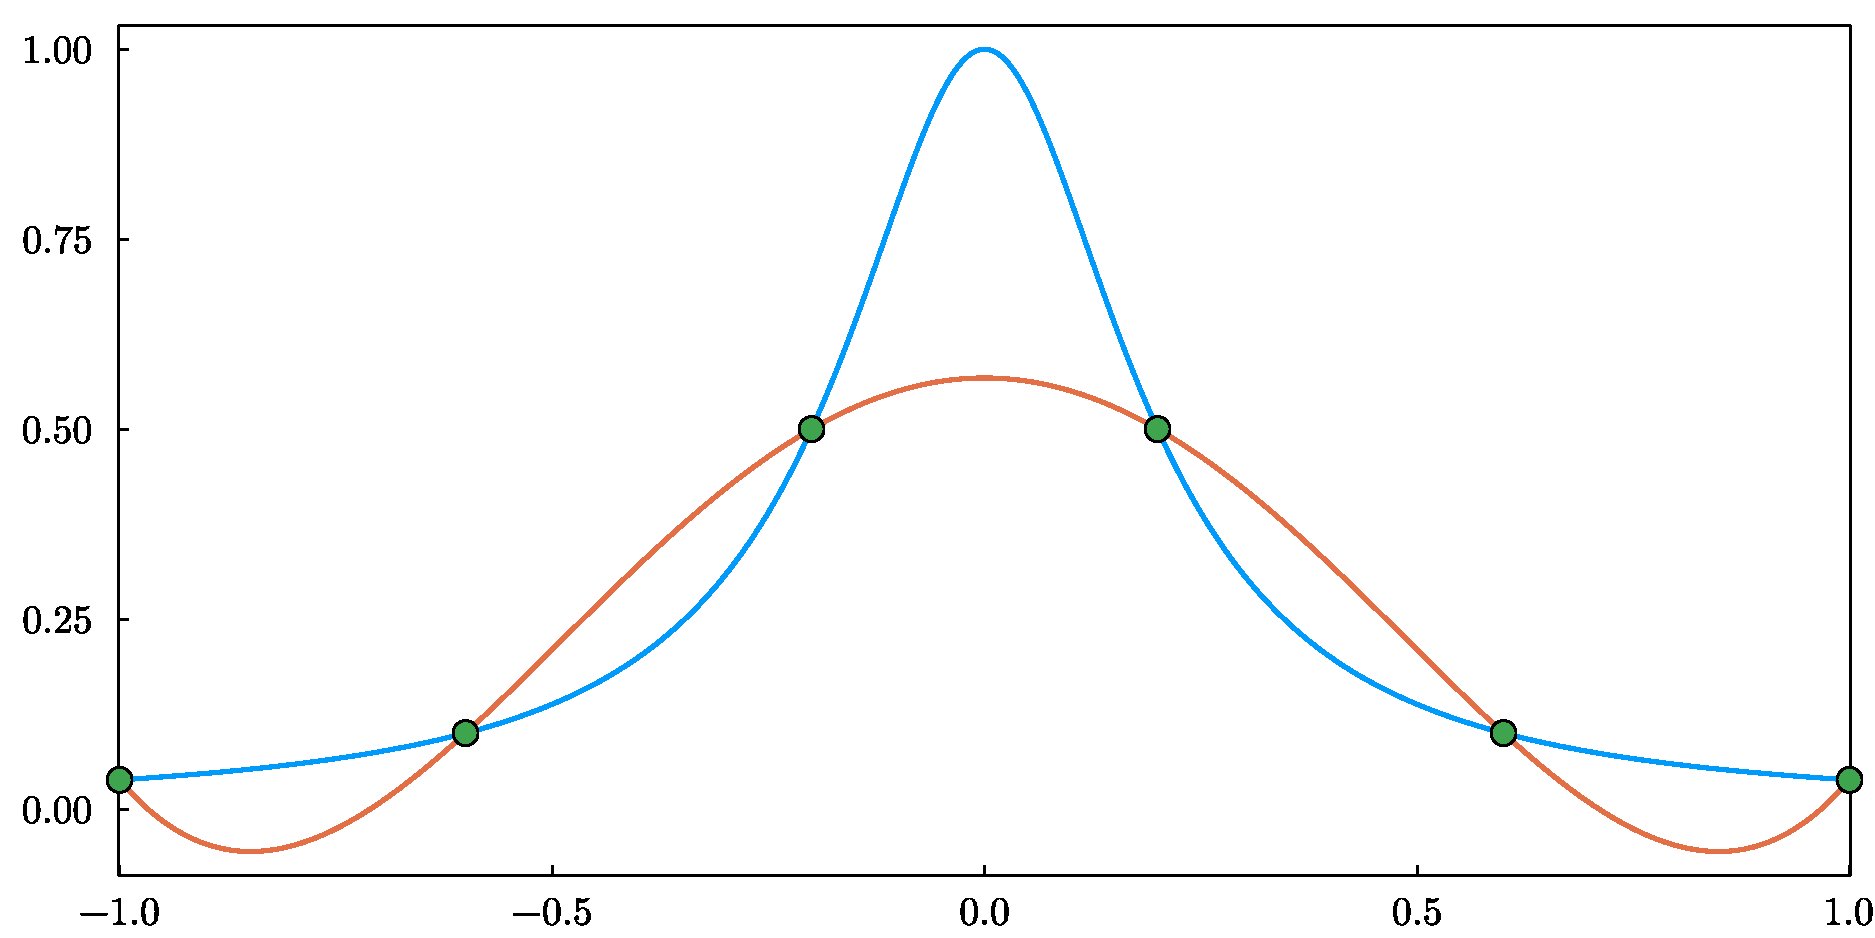
\includegraphics[width=0.49\linewidth]{figures/interpolation_runge_6.pdf}
    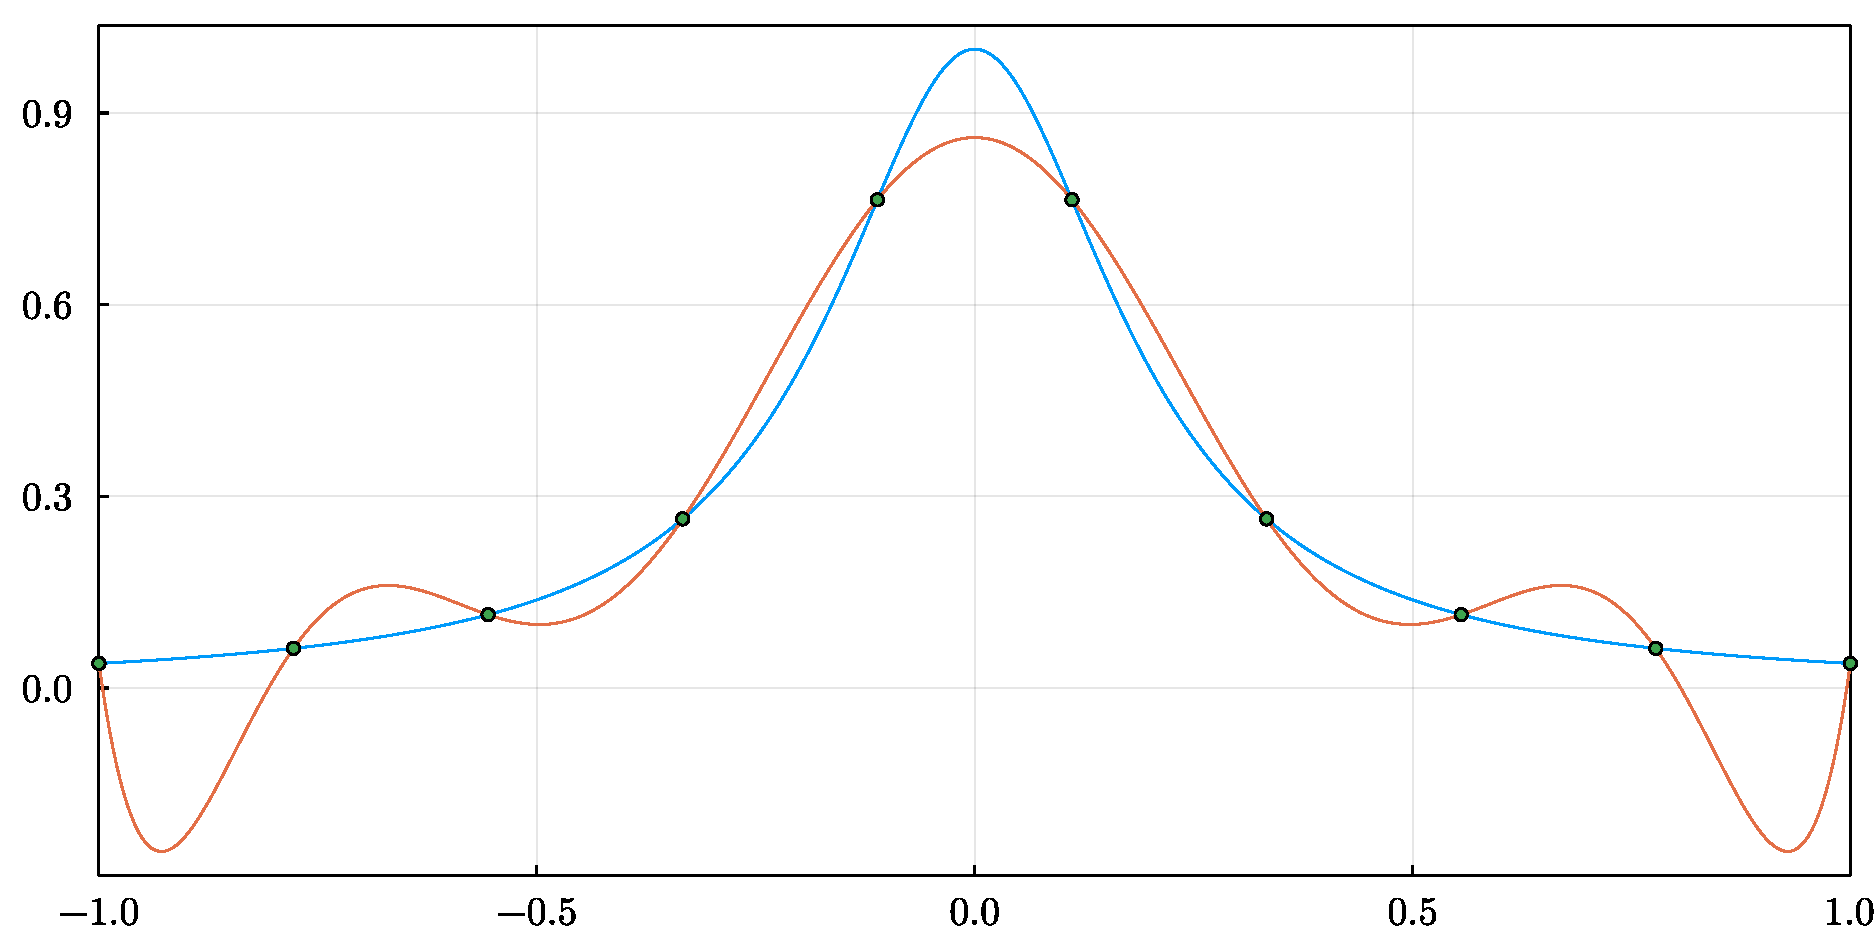
\includegraphics[width=0.49\linewidth]{figures/interpolation_runge_10.pdf}
    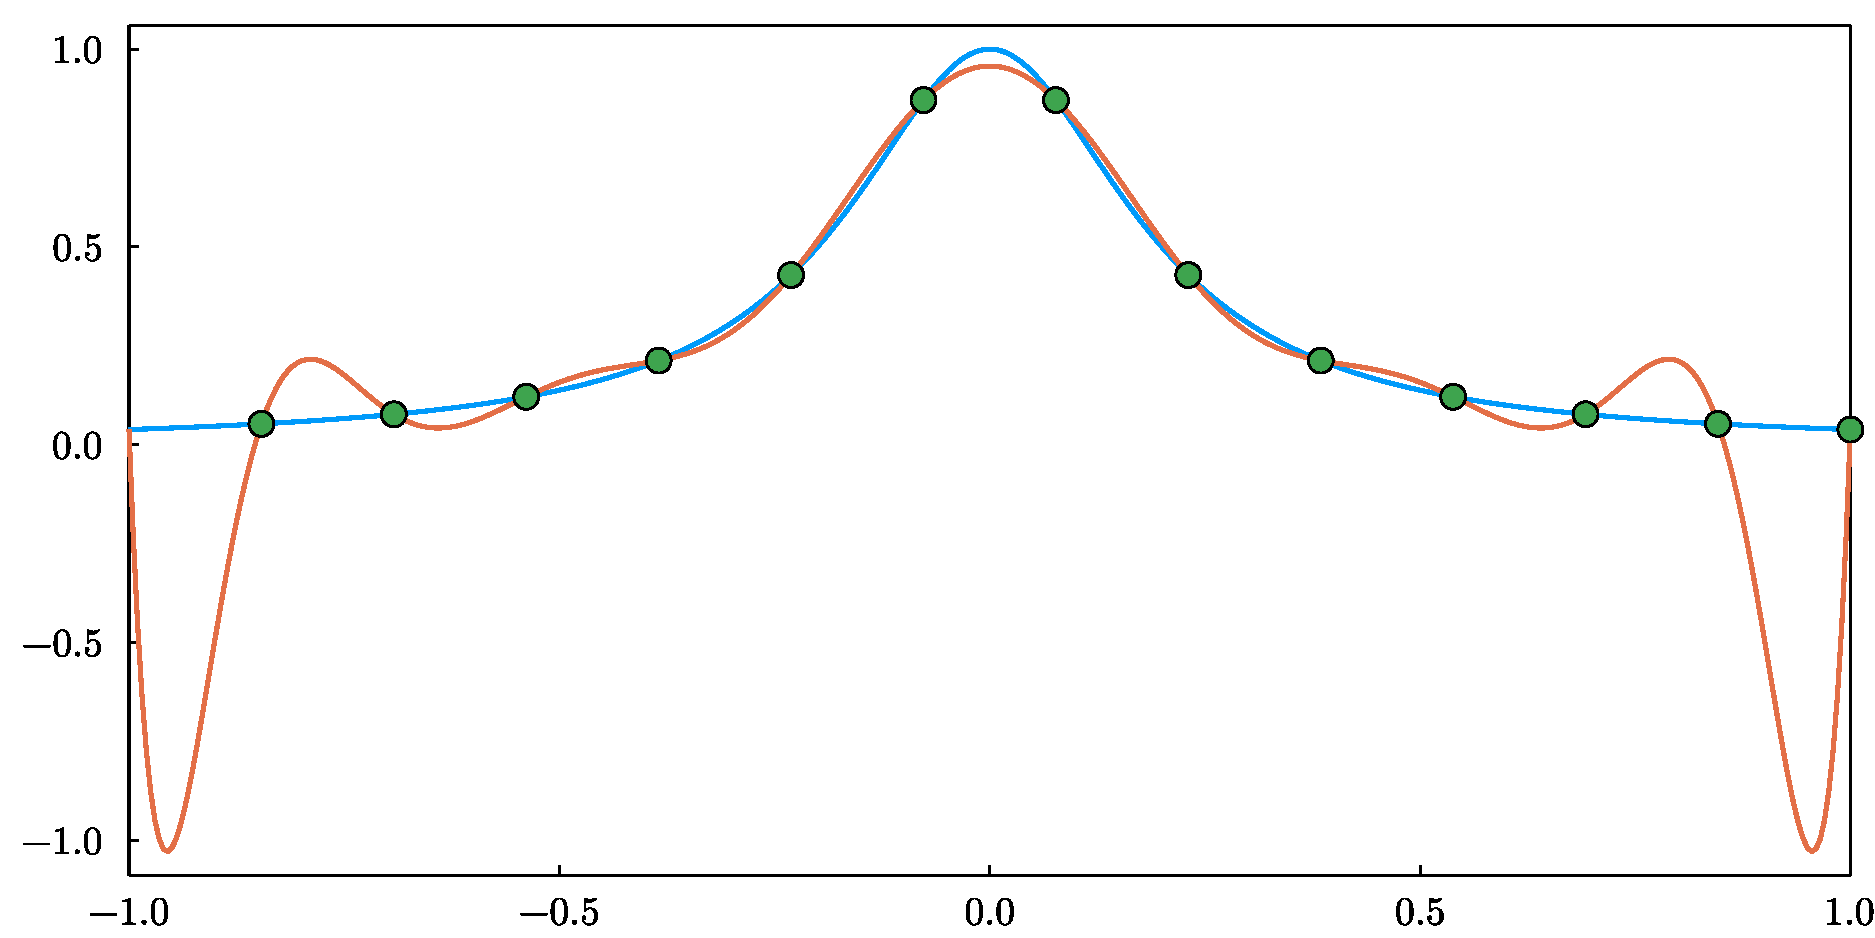
\includegraphics[width=0.49\linewidth]{figures/interpolation_runge_14.pdf}
    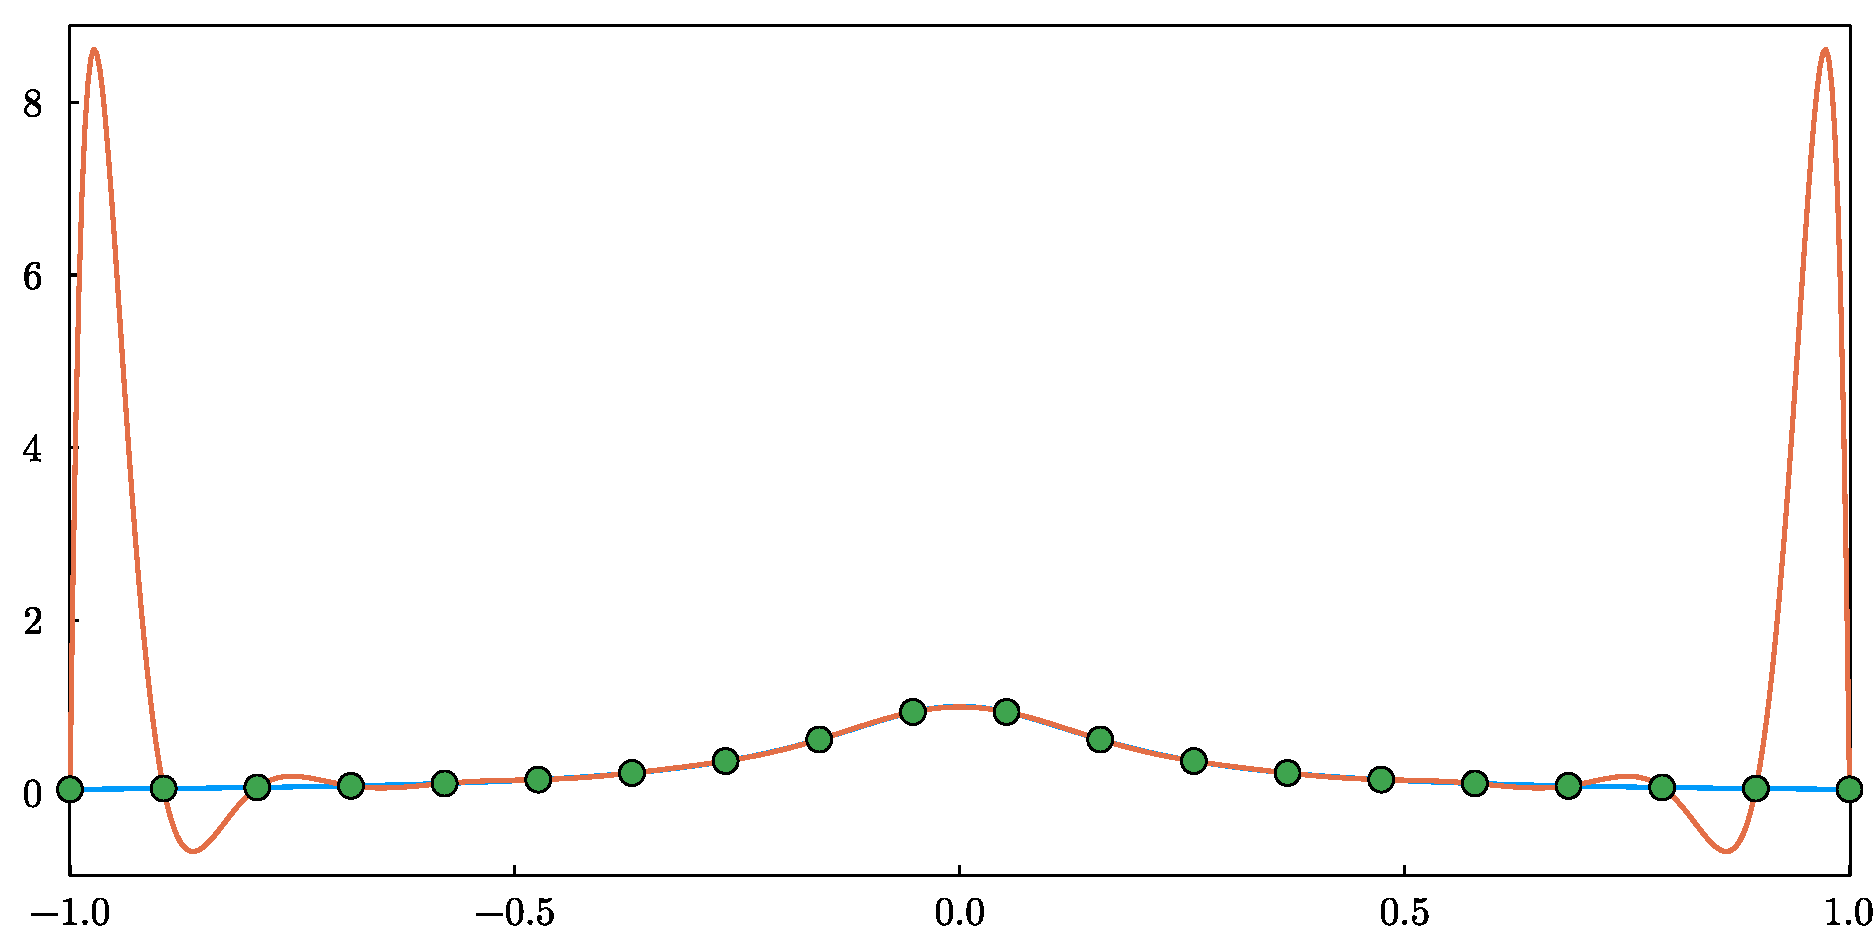
\includegraphics[width=0.49\linewidth]{figures/interpolation_runge_20.pdf}
    \caption{Interpolation (in orange) of the Runge function~\eqref{eq:runge_function} (in blue) using 6, 10, 14, and 20 equidistant nodes.}%
    \label{fig:interpolation_runge_function}
\end{figure}

\subsection{Interpolation at Chebyshev nodes}
Sometimes,
interpolation is employed as a technique for approximating functions.
The spectral collocation method, for example,
is a technique for solving partial differential equations
where a discrete solution is first calculated,
and then a continuous solution is constructed using polynomial or Fourier interpolation.
When the interpolation nodes are not given a priori as data,
it is natural to wonder whether these can be picked in such a manner that the interpolation error,
measured in a function norm, is minimized.
For example, given a continuous function~$u(x)$ and a number of nodes~$n$,
is it possible to chose nodes $x_0, \dotsc, x_n$ such that
\[
    E := \sup_{x \in [a, b]} \bigl\lvert u(x) - \widehat u(x) \bigr\rvert
\]
is minimized?
Here $\widehat u$ is the polynomial interpolating~$u$ at the nodes.
Achieving this goal in general is a difficult task,
because $\xi = \xi(x)$ is unknown in the expression of the interpolation error from~\cref{theorem:interpolation_error}:
\[
    e_n(x) = \frac{u^{(n+1)}(\xi)}{n+1!} (x-x_0) \dotsc (x - x_n).
\]
In view of this difficulty,
we will focus on the simpler problem of finding interpolation nodes
such that the product $(x-x_0) \dotsc (x - x_n)$ is minimized in the supremum norm.
This problem amounts to finding the optimal interpolation nodes,
in the sense that~$E$ is minimized,
in the particular case where $u$ is a polynomial of degree $n+1$,
because in this case $u^{(n+1)}(\xi)$ is a constant factor.
It turns out that this problem admits an explicit solution,
which we will deduce from the following theorem.
\begin{theorem}
    [Minimum $\infty$ norm]
    \label{theorem:minimum_infty_norm}
    Assume that $p$ is a monic polynomial of degree $n \geq 1$:
    \[
        p(x) = \alpha_0 + \alpha_1 x + \dotsb + \alpha_{n-1} x^{n-1} +  x^n.
    \]
    Then it holds that
    \begin{equation}
        \label{eq:chebychev_lower_bound}
        \sup_{x \in [-1, 1]} \bigl\lvert p(x) \bigr\rvert \geq \frac{1}{2^{n-1}} =: E.
    \end{equation}
    In addition, the lower bound is achieved for~$p_*(x) = 2^{-(n-1)} T_n(x)$,
    where $T_n$ is the Chebyshev polynomial of degree~$n$:
    \begin{equation}
        \label{eq:chebyshev_polynomial}
        T_n(x) = \cos(n\arccos x) \qquad (-1 \leq x \leq 1).
    \end{equation}
\end{theorem}
\begin{proof}
    By~\cref{exercise:chebyshev_leading_coefficient},
    the polynomial $x \mapsto 2^{-(n-1)} T_n(x)$ is indeed monic,
    and it is clear that it achieves the lower bound~\eqref{eq:chebychev_lower_bound}
    since $\abs{T_n(x)} \leq 1$ for all $x \in [-1, 1]$.

    In order to prove~\eqref{eq:chebychev_lower_bound},
    we assume by contradiction that there is a different monic polynomial~$q$ of degree~$n$ such that
    \begin{equation}
        \label{eq:chebyshev_minimum}
        \sup_{x \in [-1, 1]} \bigl\lvert q(x) \bigr\rvert < E.
    \end{equation}
    Let us introduce $x_i = \cos(i \pi/n)$, for $i = 0, \dotsc, n$,
    and observe that
    \[
        p(x_i) = 2^{-(n-1)} T_n(x_i) = (-1)^i E.
    \]
    The function $h(x) := p(x) - q(x)$ is a polynomial of degree at most $n-1$ which,
    by the assumption~\eqref{eq:chebyshev_minimum},
    is strictly positive at $x_0, x_2, x_4, \dotsc$ and strictly negative at $x_1, x_3, x_5, \dotsc$.
    Therefore, the polynomial $h(x)$ changes sign at least $n$ times and so,
    by the intermediate value theorem, it has at least $n$ roots.
    But this is impossible, because $h(x) \neq 0$ and $h(x)$ is of degree at most $n-1$.
\end{proof}
\begin{remark}
    [Derivation of Chebyshev polynomials]
    \label{remark:cheb}
    The polynomial~$p_*$ achieving the lower bound in~\eqref{eq:chebychev_lower_bound}
    oscillates between the values $-E$ and $E$,
    which are respectively its minimum and maximum values over the interval~$[-1, 1]$.
    It attains the values $E$ or $-E$ at $n+1$ distinct points $x_0 < \dotsc < x_n$,
    with $x_0 = -1$ and $x_n = 1$.
    It turns out that these properties,
    which can be shown to hold a priori using Chebyshev's \emph{equioscillation theorem},
    are sufficient to derive an explicit expression for the polynomial~$p_*$,
    as we formally demonstrate hereafter.

    The points $x_2, \dotsc, x_{n-1}$
    are local extrema of~$p_*$,
    and so~$p_*'(x) = 0$ at these nodes.
    We therefore deduce that $p_*$ satisfies the differential equation
    \begin{equation}
        \label{eq:differential_equation_chebyshev}
        n^2\left(E^2 - p_*(x)^2\right) = p_*'(x)^2 (1 - x^2).
    \end{equation}
    Indeed, both sides are polynomials of degree $2n$ with single roots at -1 and 1,
    with double roots at $x_2, \dotsc, x_{n+1}$,
    and with the same coefficient of the leading power.
    In order to solve~\eqref{eq:differential_equation_chebyshev},
    we rearrange the equation and take the square root:
    \[
        \frac{\frac{p_*'(x)}{E}}{\sqrt{1 - \frac{p_*(x)^2}{E^2}}} = \pm \frac{n}{1 - x^2}
        \qquad \Leftrightarrow \qquad
        \frac{\d}{\d x} \left( \arccos\left(\frac{p_*(x)}{E}\right) \right) = \pm n \frac{\d}{\d x} \arccos(x).
    \]
    Integrating both sides and taking the cosine,
    we obtain
    \[
        p_*(x) = E \cos\bigl(C + n \arccos(x)\bigr).
    \]
    Requiring that $|p_*(-1)| = E$, we deduce $C = 0$.
\end{remark}

From~\cref{theorem:minimum_infty_norm},
we deduce the following corollary.
\begin{corollary}
    [Chebyshev nodes]
    \label{corollary:chebyshev_nodes}
    Assume that $x_0 < x_1 < \dotsc < x_n$ are in the interval $[a, b]$.
    The supremum norm of the product $\omega(x) := (x-x_0) \dotsb (x-x_n)$ over~$[a, b]$ is minimized when
    \begin{equation}
        x_i = a + (b-a) \frac{1 + \cos \left( \frac{(2i + 1) \pi}{2(n+1)} \right)}{2}
    \end{equation}
        % \label{eq:optimal_product}
        % (x-x_0) \dotsb (x-x_n) = \frac{(b-a)^n}{2^{2n-1}} T_n\left(\frac{a + b - 2x}{a - b}\right).
    % \end{equation}
    % In particular, if $a = -1$ and $b = 1$,
    % then the nodes $x_0, \dotsc, x_n$ must coincide with the roots of the Chebyshev polynomial of degree~$n$:
    % \[
        % x_i = \cos \left( (2i + 1) \frac{\pi}{2} \right).
    % \]
\end{corollary}
\begin{proof}
    We consider the affine change of variable
    \begin{align*}
        \zeta\colon &[-1, 1] \to [a, b]; \\
                    &y \mapsto \frac{a + b + y (b - a)}{2}.
    \end{align*}
    The function
    \begin{align*}
        p(y) &:= \frac{2^n}{(b-a)^n} \omega\bigl(\zeta(y)\bigr) = \frac{2^{n+1}}{(b-a)^{n+1}} \bigl(\zeta(y)-x_0\bigr) \dotsb \bigl(\zeta(y)-x_n\bigr) \\
             &= \bigl(y-y_0\bigr) \dotsb \bigl(y-y_n\bigr), \qquad y_i = \zeta^{-1}(x_i),
    \end{align*}
    is a monic polynomial of degree~$n+1$ such that
    \begin{equation}
        \label{eq:change_of_variable}
        \sup_{y \in [-1, 1]} \abs{p(y)} = \frac{2^{n+1}}{(b-a)^{n+1}} \sup_{x \in [a, b]} \abs{(x-x_0) \dotsc (x - x_n)}.
    \end{equation}
    By~\cref{theorem:minimum_infty_norm},
    the left-hand side is minimized when $p$ is equal to $2^{-n} T_{n+1}(y)$,
    i.e.\ when the roots of $p$ coincide with the roots of $T_{n+1}$.
    This occurs when
    \[
        y_i = \zeta^{-1}(x_i) = \cos \left( \frac{(2i + 1)\pi}{2 (n+1)} \right).
    \]
    Applying the inverse change of variable $x_i = \zeta(y_i)$,
    we deduce the result.
\end{proof}

\Cref{corollary:chebyshev_nodes} is useful for interpolation.
The nodes
\begin{equation}
    x_i = a + (b-a) \frac{1 + \cos \left( (2i + 1) \frac{\pi}{2 n} \right)}{2}, \qquad i = 0, \dotsc, n,
\end{equation}
are known as Chebyshev nodes and,
more often than not, employing these nodes for interpolation produces much better results than using equidistant rodes,
both in the case where~$u$ is a polynomial of degree $n+1$,
as we just proved,
but also for general~$u$.
As an example we plot in \cref{fig:cheb_runge} the interpolation of the Runge function using Chebyshev nodes.
In this case, the interpolating polynomial converges uniformly to the Runge function as we increase the number of interpolation nodes!
\begin{figure}[ht]
    \centering
    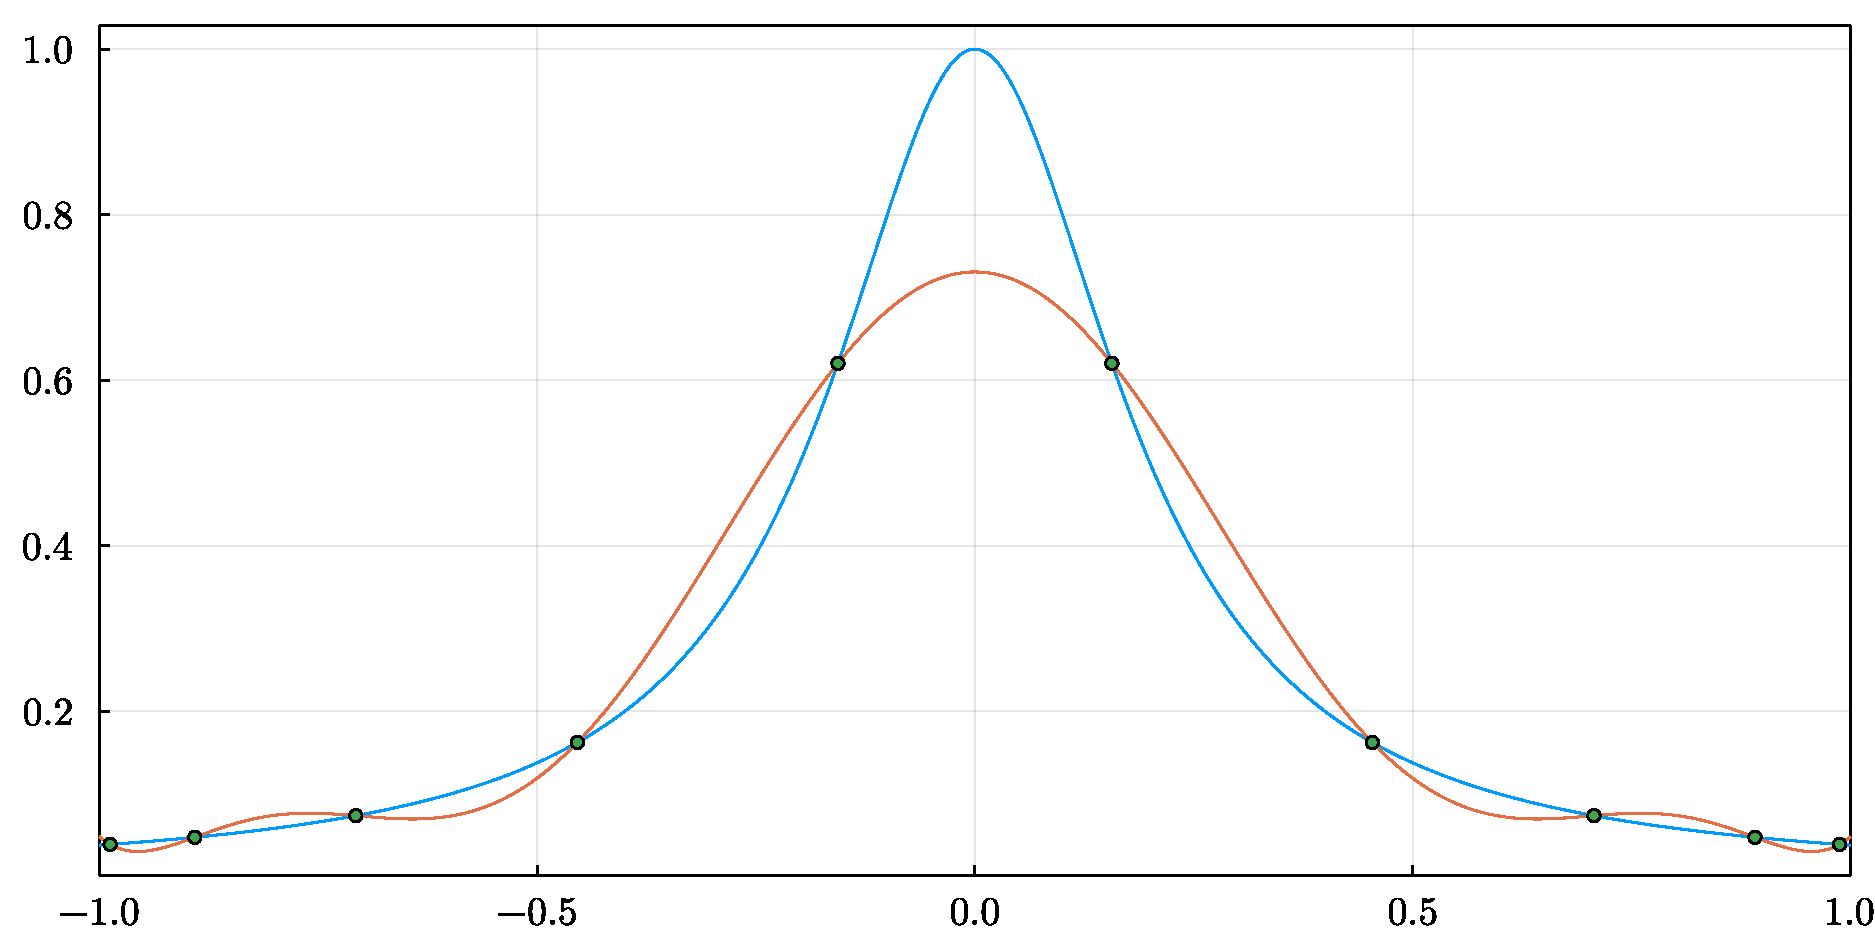
\includegraphics[width=0.49\linewidth]{figures/interpolation_cheb_runge_10.pdf}
    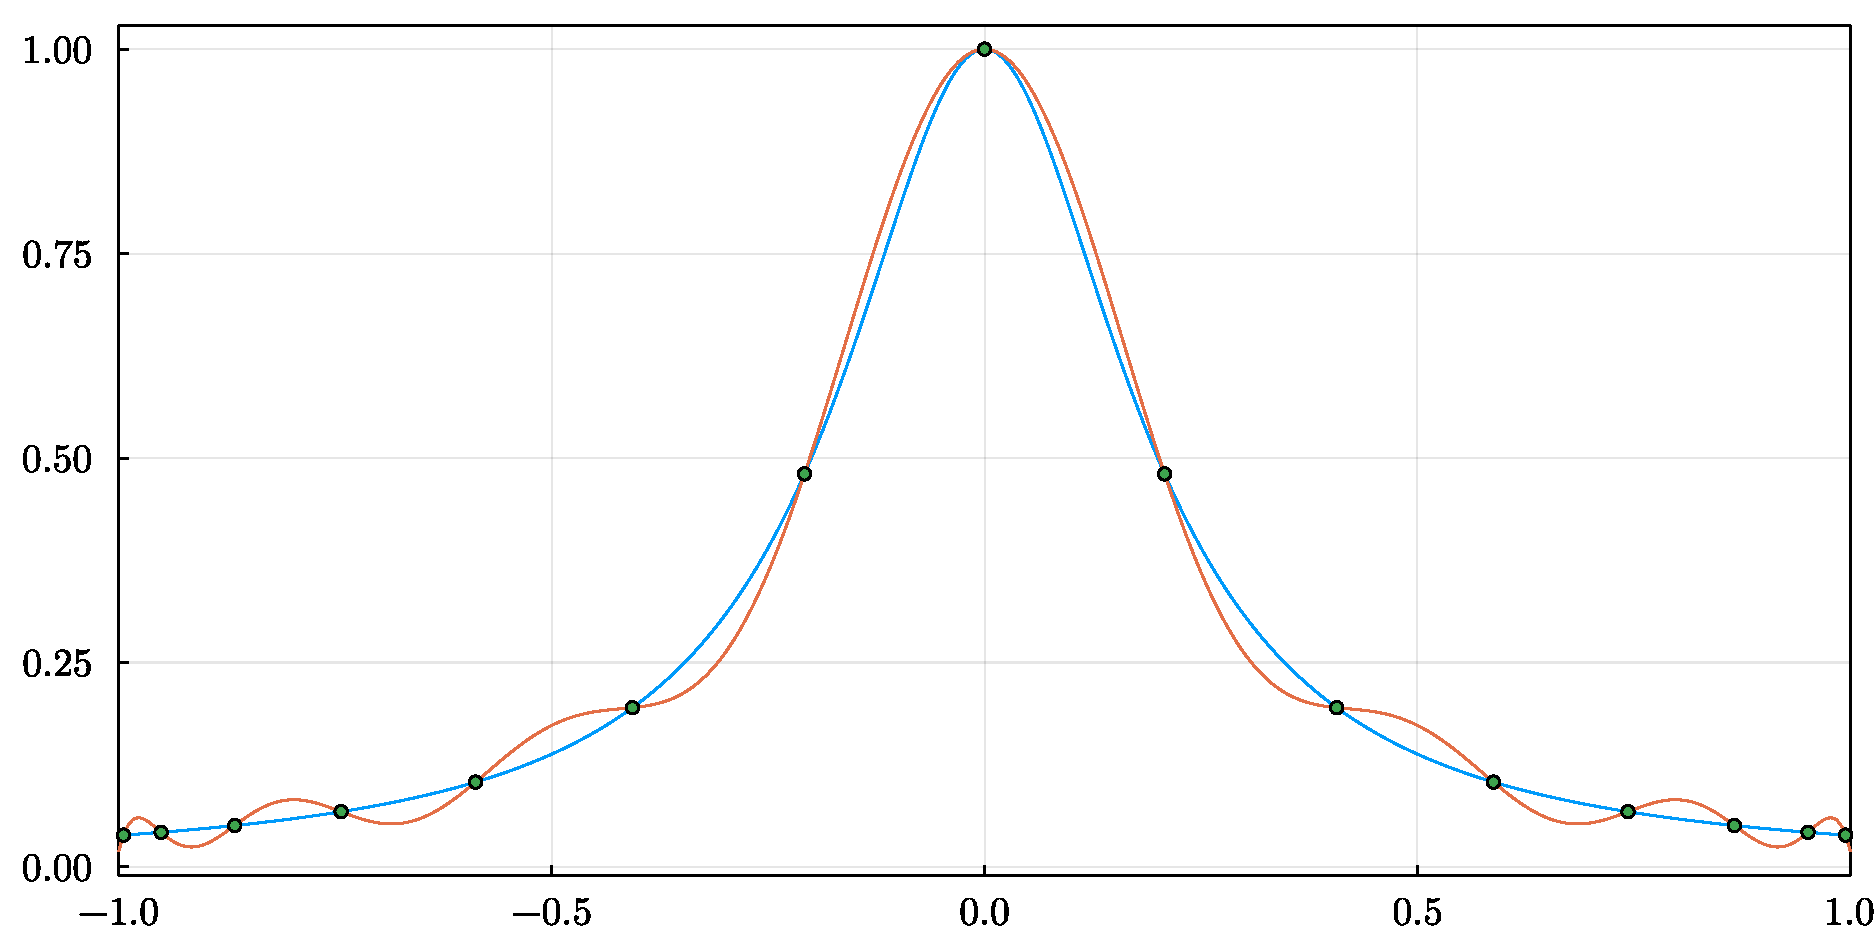
\includegraphics[width=0.49\linewidth]{figures/interpolation_cheb_runge_15.pdf}
    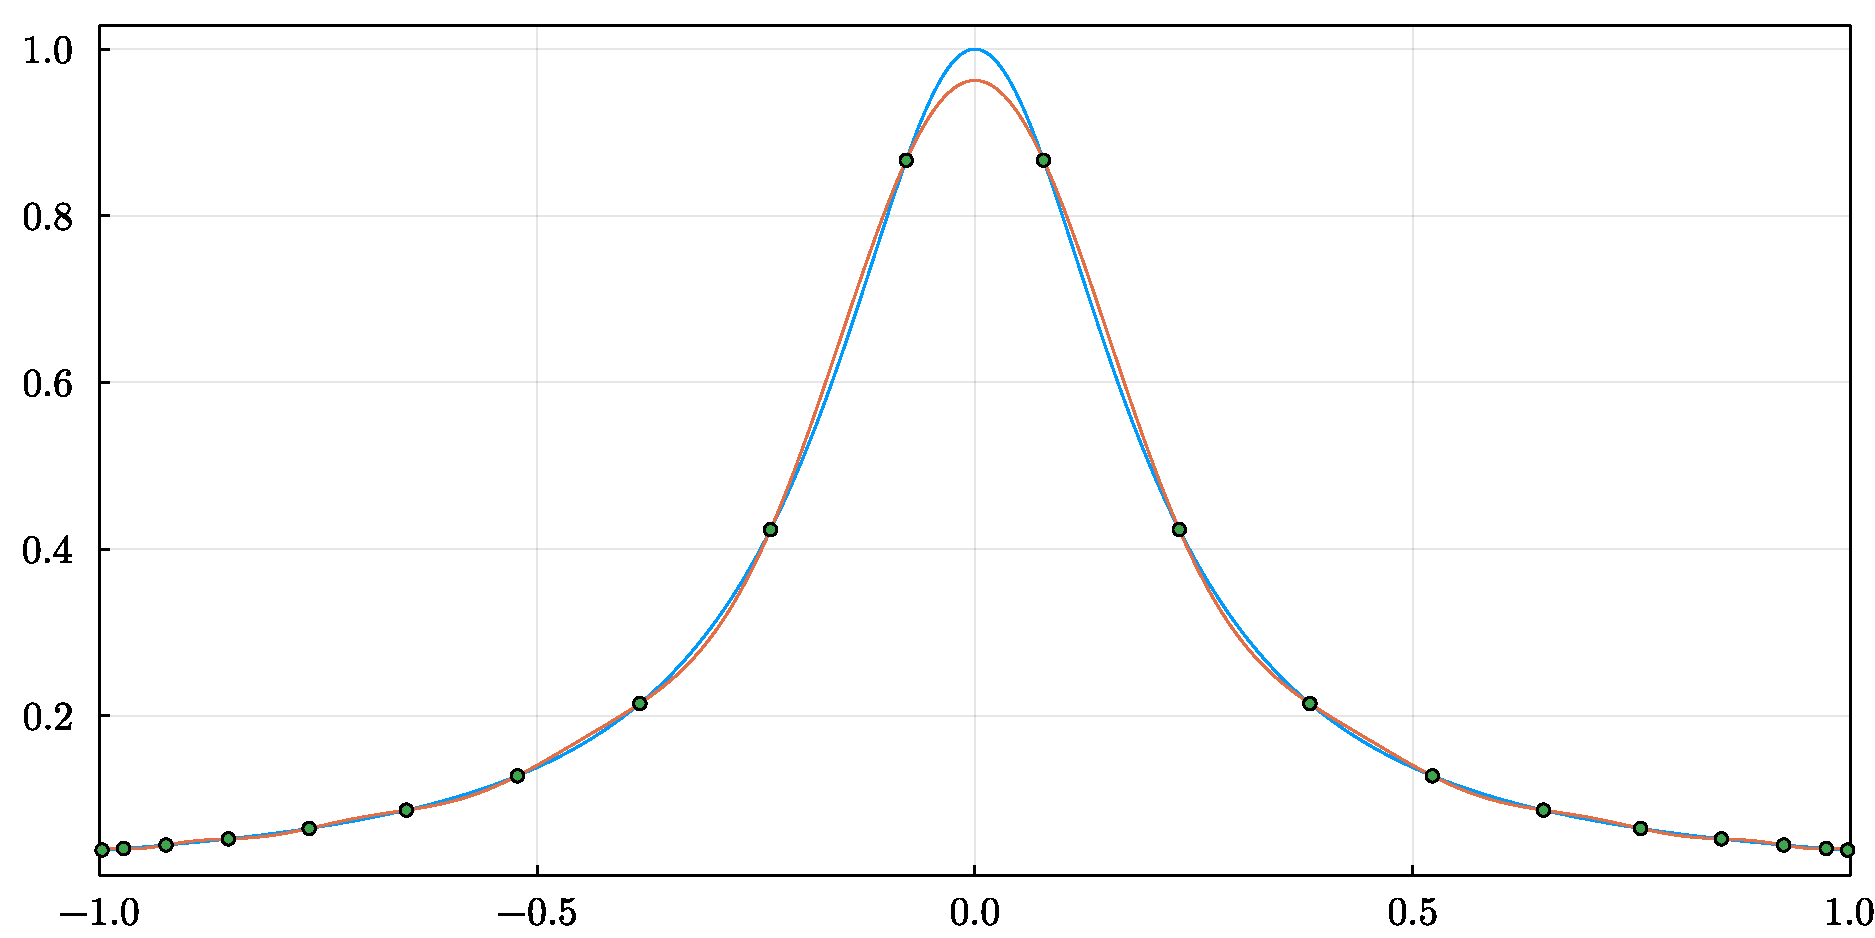
\includegraphics[width=0.49\linewidth]{figures/interpolation_cheb_runge_20.pdf}
    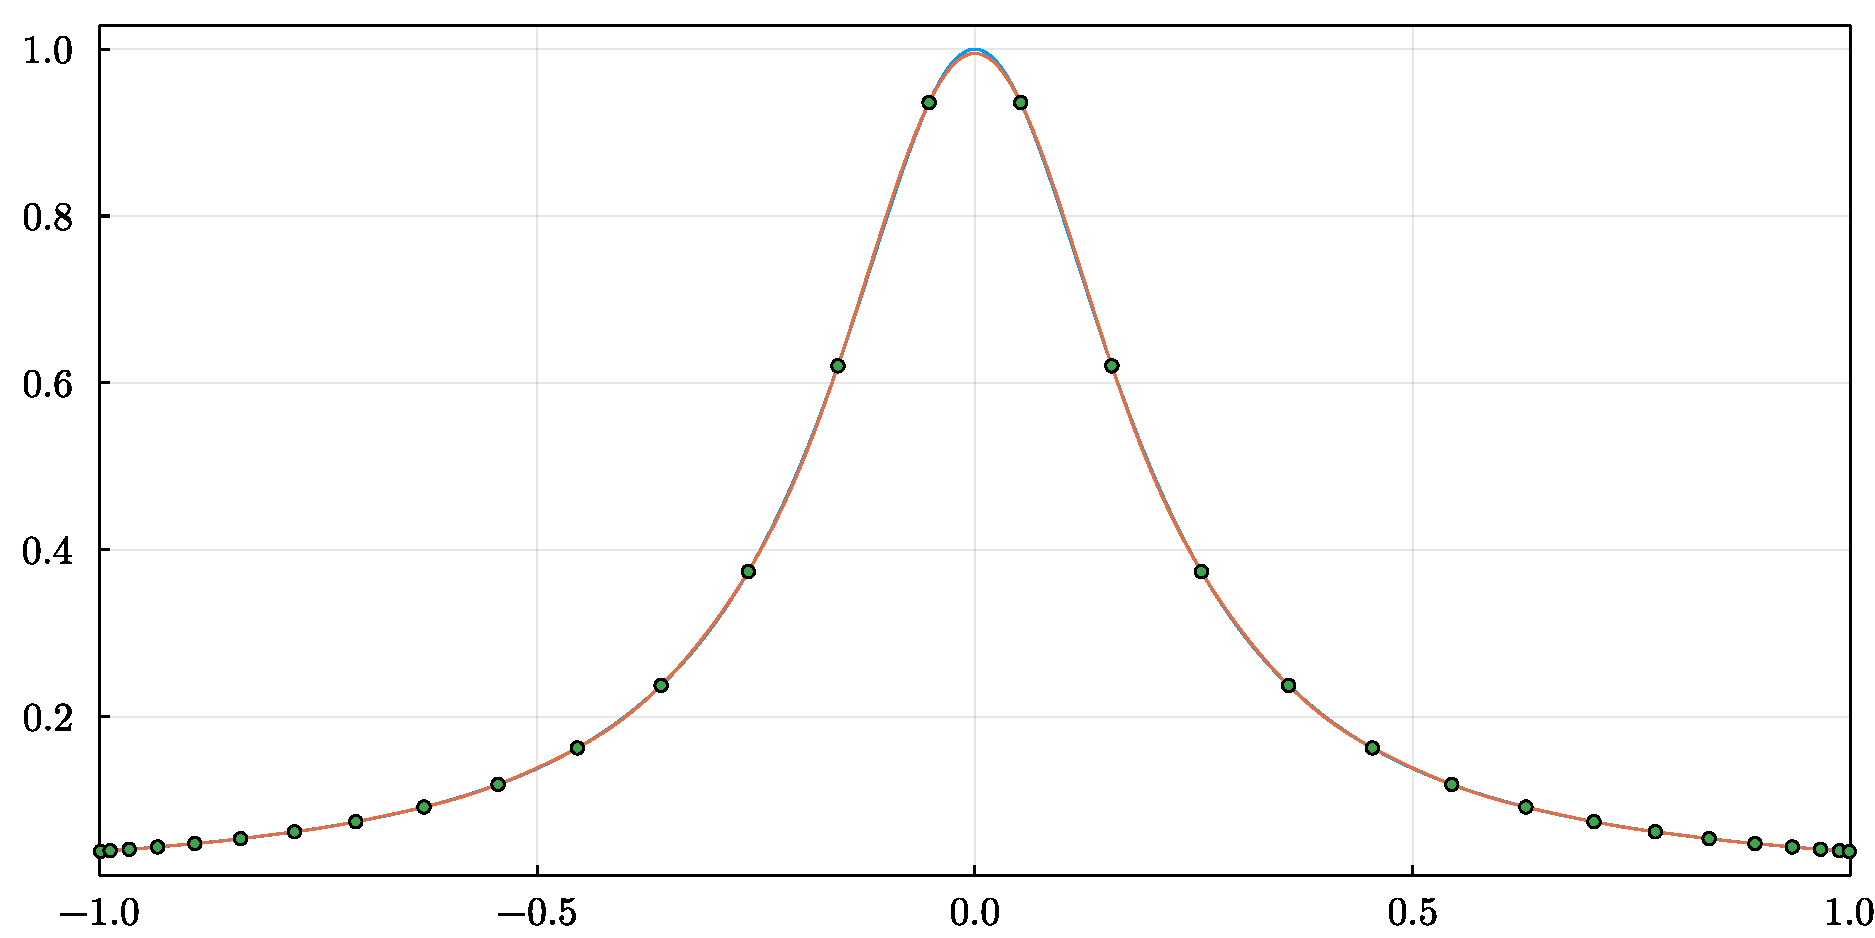
\includegraphics[width=0.49\linewidth]{figures/interpolation_cheb_runge_30.pdf}
    \caption{Interpolation (in orange) of the Runge function~\eqref{eq:runge_function} (in blue) using 10, 15, 20, and~30 Chebyshev nodes.}%
    \label{fig:cheb_runge}
\end{figure}

\subsection{Hermite interpolation}
Hermite interpolation,
sometimes also called Hermite--Birkoff interpolation,
generalizes Lagrange interpolation to the case where,
in addition to the function values $u_0, \dotsc, u_n$,
the values of some of the derivatives are given at the interpolation nodes.
For simplicity,
we assume in this section that only the first derivative is specified.
In this case, the aim of Hermite interpolation is to find,
given data~$(x_i, u_i, u_i')$ for $i \in \{0, \dotsc, n\}$,
a polynomial~$\widehat u$ of degree at most~$2n + 1$ such that
\[
    \forall i \in \{0, \dotsc, n\}, \qquad
    \widehat u(x_i) = u_i, \qquad
    \widehat u'(x_i) = u'_i.
\]
In order to construct the interpolating polynomial,
it is useful to define the functions
\[
    \psi_{i}(x)
    = \prod_{j=0, j\neq i}^{n} \left( \frac{x-x_j}{x_i-x_j} \right)^2,
    \qquad i = 0, \dotsc, n.
\]
The function $\psi_i$ is the square of the usual Lagrange polynomials associated with~$x_i$,
and it satisfies
\[
    \psi_i(x_j) = 1,
    \qquad \psi_i'(x_i) = \sum_{j=0,j\neq i}^{n} \frac{2}{x_i - x_j},
    \qquad \forall j \neq i \qquad \psi_i(x_j) = \psi_i'(x_j) = 0.
\]
We consider the following ansatz for~$\widehat u$:
\[
    \widehat u(x) = \sum_{i=0}^{n} \psi_i(x) q_i(x),
\]
where $q_i$ are polynomials to be determined of degree at most one,
so that~$\widehat u$ is of degree at most~$2n+1$.
We then require
\[
    \widehat u(x_i) = q_i(x_i), \qquad \widehat u'(x_i) = \psi_i'(x_i) q(x_i) + q'(x_i).
\]
From the first equation, we deduce that $q_i(x_i) = u_i$,
and from the second equation we then have~$q'(x_i) = \widehat u'(x_i) - \psi_i'(x_i) u_i$.
We conclude that the interpolating polynomial is given by
\[
    \widehat u(x) = \sum_{i=0}^{n} \psi_i(x) \Bigl(u_i + \bigl(u_i' - \psi_i'(x_i) u_i\bigr) (x - x_i)\Bigr).
\]
The following theorem gives an expression of the error.
\begin{theorem}
    [Hermite interpolation error]
    \label{theorem:hermite_interpolation}
    Assume that~$u\colon [a, b] \to \real$ is a function in $C^{2n+2}([a, b])$ and let~$\widehat u$
    denote the Hermite interpolation of~$u$ at the nodes~$x_0, \dotsc, x_n$.
    Then for all $x \in [a, b]$,
    there exists~$\xi = \xi(x)$ in the interval $[a, b]$ such that
    \[
        u(x) - \widehat u(x) = \frac{u^{(2n+2)}(\xi)}{(2n+2)!} (x-x_0)^2 \dotsc (x - x_n)^2.
    \]
\end{theorem}
\begin{proof}
    See~\cref{exercise:proof_hermite}.
\end{proof}

\subsection{Piecewise interpolation}
\label{sub:piecewise_interpolation}
The interpolation methods we discussed so far are in some sense global;
they aim to construct one polynomial that goes through all the data points.
This approach is attractive because the interpolant is infinitely smooth but,
as we observed, it is not always fruitful,
in particular when equidistant interpolation nodes are employed.
An alternative approach is to divide the domain in a number of small intervals
and perform polynomial interpolation within each interval.
Although the resulting interpolating function is usually not smooth over the full domain,
this ``local'' approach to interpolation is more robust.

Several methods belong in the category of piecewise interpolation.
We mention, for instance, piecewise Lagrange interpolation and cubic splines interpolation.
In this section,
we briefly describe the former method,
which is widely used in the context of the \emph{finite element method}.
Information on the latter method is available in~\cite[Section 8.7.1.]{MR2265914}.

For simplicity, we illustrate the method in dimension 1,
but piecewise Lagrange interpolation can be extended to several dimensions.
Assume that we wish to approximate a function~$u\colon [a, b] \to \real$.
We consider a subdivision $a = x_0 < x_1 < \dotsc < x_n = b$ of the interval $[a, b]$
and let~$h$ denote the maximum spacing:
\[
    h = \max_{i \in \{0, \dotsc, n-1\}} \abs{x_{i+1} - x_i}.
\]
Within each subinterval $I_i = [x_i, x_{i+1}]$,
we consider a further subdivision
\[
    x_i = x_i^{(0)} < x_i^{(1)} < \dotsc < x_i^{(m)} = x_{i+1},
\]
where the nodes $x_i^{(0)}, \dotsc, x_i^{(m)}$ are equally spaced with distance $h/m$.
The idea of piecewise Lagrange interpolation is to calculate,
for each interval $I_i$ in the partition,
the interpolating polynomial~$p_i$ at the nodes $x_i^{(0)}, \dotsc, x_i^{(m)}$.
The interpolant is then defined as
\begin{equation}
    \label{eq:piecewise_interpolation}
    \widehat u(x) = p_{\iota}(x),
\end{equation}
where $\iota = \iota(x)$ is the index of the interval to which $x$ belongs.
Since $x_i^{(m)} = x_{i+1} = x_{i+1}^{(0)}$,
the interpolant defined by~\eqref{eq:piecewise_interpolation} is continuous.
If the function $u$ belongs to $C^{m+1}([a, b])$,
then by~\cref{corollary:interpolation_error} the interpolation error within each subinterval may be bounded from above as follows:
\begin{equation}
    \label{eq:error_estimate_piecewise_interpolation}
    \sup_{x \in I_i} \abs{u(x) - \widehat u(x)} \leq \frac{ C_{m+1} (h/m)^{m+1}}{4(m + 1)},
    \qquad C_{m+1} := \sup_{x \in [a, b]} \abs{u^{(m+1)}(x)},
\end{equation}
and so we deduce
\begin{equation*}
    \sup_{x \in [a, b]} \abs{u(x) - \widehat u(x)} \leq C h^{m+1},
\end{equation*}
for an appropriate constant~$C$ independent of $h$.
This equation shows that the error is guaranteed to decrease to~0 in the limit as $h \to \infty$.
In practice, the number $m$ of interpolation nodes within each interval can be small.
% Several integration methods presented~\cref{cha:quadrature} are related to piecewise interpolation.

\section{Approximation}
In this section,
we focus on the subject of \emph{approximation},
both of discrete data points and of continuous functions.
We begin, in \cref{sub:polynomial_regression} with a discussion of least squares approximation for data points,
and in \cref{sub:mean_square_approximation} we focus on function approximation in the mean square sense.

\subsection{Least squares approximation of data points}
\label{sub:polynomial_regression}
Consider $n + 1$ distinct $x$ values $x_0 < \dotsc < x_n$,
and suppose that we know the values $u_0, \dotsc, u_n$ taken by an unknown function $u$ when evaluated at these points.
We wish to approximate the function~$u$ by a function of the form
\begin{equation}
    \label{eq:expansion_approx}
    \widehat u(x) = \sum_{i=0}^{m} \alpha_i \varphi_i(x) \in \Span \{ \varphi_0, \dotsc, \varphi_m \},
\end{equation}
for some $m < n$.
In many cases of practical interest,
the basis functions $\varphi_0, \dotsc, \varphi_m$ are polynomials.
In contrast with interpolation,
here we seek a function $\widehat u$ in a finite-dimensional function space of dimension~$m$ strictly lower than the number of data points.
In order for~$\widehat u$ to be a good approximation,
we wish to find coefficients $\alpha_0, \dotsc, \alpha_m$ such that
the following linear system is approximately satisfied.
\[
    \mat A \vect \alpha :=
    \begin{pmatrix}
        \varphi_0(x_0) & \varphi_1(x_0) & \hdots & \varphi_m(x_0) \\
        \varphi_0(x_1) & \varphi_1(x_1) & \hdots & \varphi_m(x_1) \\
        \varphi_0(x_2) & \varphi_1(x_2) & \hdots & \varphi_m(x_2) \\
        \vdots & \vdots & & \vdots \\
        \varphi_0(x_{n-2}) & \varphi_1(x_{n-2}) & \hdots & \varphi_m(x_{n-2}) \\
        \varphi_0(x_{n-1}) & \varphi_1(x_{n-1}) & \hdots & \varphi_m(x_{n-1}) \\
        \varphi_0(x_n) & \varphi_1(x_n) & \hdots & \varphi_m(x_n)
    \end{pmatrix}
    \begin{pmatrix}
        \alpha_0 \\
        \alpha_1 \\
        \vdots \\
        \alpha_m
    \end{pmatrix}
    \approx
    \begin{pmatrix}
        u_0 \\
        u_1 \\
        u_2 \\
        \vdots \\
        u_{n-2} \\
        u_{n-1} \\
        u_n
    \end{pmatrix} =: \vect b.
\]
In general,
since the matrix on the left-hand side has more lines than columns,
there does not exist an exact solution to this equation.
In order to find an approximate solution,
a natural approach is to find coefficients $\alpha_0, \dotsc, \alpha_m$ such that
the residual vector $\vect r = \mat A \vect \alpha - \vect b$ is small in some vector norm.
A particularly popular approach,
known as least squares approximation,
is to minimize the Euclidean norm of~$\vect r$ or,
equivalently, the square of the Euclidean norm:
\[
    \norm{\vect r}^2 = \sum_{i=0}^{n} \abs[big]{u_i - \widehat u(x_i)}^2 = \sum_{i=0}^{n} \left( u_i - \sum_{j=0}^{m} \alpha_j \varphi_j(x_i) \right)^2.
\]
Let us denote the right-hand side of this equation by~$J(\vect \alpha)$,
which we view as a function of the vector of coefficients $\vect a$.
A necessary condition for~$\vect a_*$ to be a minimizer is that $\nabla J(\vect \alpha_*) = 0$.
The gradient of $J$,
written as a column vector, is given by
\begin{align*}
    \nabla J(\vect \alpha)
    &= \nabla \Bigl( (\mat A \vect \alpha - \vect b)^\t (\mat A \vect \alpha - \vect b) \Bigr) \\
    &= \nabla \Bigl( \vect \alpha^\t (\mat A^\t \mat A) \vect \alpha - \vect b \mat A  \vect \alpha - \vect \alpha^\t \mat A^\t \vect b + \vect b^\t \vect b) \Bigr) \\
    &= 2 (\mat A^\t \mat A) \vect \alpha - 2 \mat A^\t \vect b.
\end{align*}
We deduce that $\vect \alpha_*$ solves the linear system
\begin{equation}
    \label{eq:normal_equation}
    \mat A^\t \mat A \vect \alpha_* = \mat A^\t \vect b,
\end{equation}
where the matrix on the left-hand side is given by:
\[
    \mat A^\t \mat A :=
    \begin{pmatrix}
        \sum_{i=0}^{n} \varphi_0(x_i) \varphi_0(x_i) & \sum_{i=0}^{n} \varphi_0(x_i) \varphi_1(x_i) & \hdots & \sum_{i=0}^{n} \varphi_0(x_i) \varphi_m(x_i) \\
        \sum_{i=0}^{n} \varphi_1(x_i) \varphi_0(x_i) & \sum_{i=0}^{n} \varphi_1(x_i) \varphi_1(x_i) & \hdots & \sum_{i=0}^{n} \varphi_1(x_i) \varphi_m(x_i) \\
        \vdots & \vdots & & \vdots \\
        \sum_{i=0}^{n} \varphi_m(x_i) \varphi_0(x_i) & \sum_{i=0}^{n} \varphi_m(x_i) \varphi_1(x_i) & \hdots & \sum_{i=0}^{n} \varphi_m(x_i) \varphi_m(x_i)
    \end{pmatrix}.
\]
Equation~\eqref{eq:normal_equation} is a system of~$m$ equations with $m$ unknowns,
which admits a unique solution provided that $\mat A^\t \mat A$ is full rank or,
equivalently, the columns of~$\mat A$ are linearly independent.
The linear equations~\eqref{eq:normal_equation} are known as the \emph{normal equations}.
As a side note,
we mention that
the solution $\vect \alpha_* = (\mat A^\t \mat A)^{-1} \mat A^\t \vect b$
coincides with the maximum likelihood estimator for $\alpha$ under the assumption that the data is generated according to
$u_i = u(x_i) + \varepsilon_i$, for some function $u \in \Span \{\varphi_0, \dotsc, \varphi_m\}$
and random noise $\varepsilon_i \sim \mathcal N(0, 1)$.

\begin{remark}
From equation~\eqref{eq:normal_equation} we deduce that
\[
    \mat A \vect \alpha_* = \mat A (\mat A^\t \mat A)^{-1} \mat A^\t \vect b.
\]
The matrix~$\Pi_{\mat A} := \mat A (\mat A^\t \mat A)^{-1} \mat A^\t$ on the right-hand side is the orthogonal projection operator onto $\col(\mat A) \subset \real^n$,
the subspace spanned by the columns of~$\mat A$.
Indeed, it holds that $\Pi_{\mat A}^2 = \Pi_{\mat A}$,
which is the defining property of a projection operator.
\end{remark}

To conclude this section,
we note that the matrix $\mat A^{+} = (\mat A^\t \mat A)^{-1} \mat A^\t$ is a left inverse of the matrix $\mat A$,
because $\mat A^+ \mat A = \mat I$.
It is also called the Moore--Penrose inverse or pseudoinverse of the matrix~$\mat A$,
which generalizes the usual inverse matrix.
In Julia, the backslash operator silently uses the Moore--Penrose inverse when employed with a rectangular matrix.
Therefore, solving the normal equations~\eqref{eq:normal_equation} can be achieved by just writing \julia{α = A\b}.

\subsection{Mean square approximation of functions}
\label{sub:mean_square_approximation}
The approach described in~\cref{sub:polynomial_regression} can be generalized to the setting where the actual function~$u$,
rather than just discrete evaluations of it, is available.
In this section, we seek an approximation of the form~\eqref{eq:expansion_approx}
such that the error $\widehat u(x) - u(x)$, measured in some function norm,
is minimized.
Of course, the solution to this minimization problem depends in general on the norm employed,
and may in some cases not even be unique.
Instead of specifying a particular norm,
as done in \cref{sub:polynomial_regression},
in this section we retain some generality and assume only that the norm is induced by an inner product on the space of real-valued continuous functions:
\begin{equation}
    \label{eq:inner_product_approx}
    \ip{\placeholder,\placeholder} \colon C([a,b]) \times C([a, b]) \to \real.
\end{equation}
In other words,
we seek to minimize
\[
    J(\vect \alpha) := \norm{\widehat u - u}^2 = \ip{\widehat u - u, \widehat u - u}.
\]
This is again a function of the $m+1$ variables $\alpha_0, \dotsc, \alpha_m$.
Before calculating its gradient,
we rewrite the function $J(\vect \alpha)$ in a simpler form:
\begin{align*}
    J(\vect \alpha)
    &= \ip*{u - \sum_{j=0}^{m} \alpha_j \varphi_j,u - \sum_{k=0}^{m} \alpha_k \varphi_k} \\
    &= \sum_{j=0}^{m} \sum_{k=0}^{m} \alpha_j \alpha_k \ip{\varphi_j,\varphi_k}- 2 \sum_{j=0}^{m} \alpha_j \ip{u,\varphi_j} - \ip{u,u}
    = \vect \alpha^\t \mat G \vect \alpha - 2 \vect b^\t \vect \alpha - \ip{u,u},
\end{align*}
where we introduced
\begin{equation}
    \label{eq:approx_matrix_m}
    \mat G :=
    \begin{pmatrix}
        \ip{\varphi_0, \varphi_0} & \ip{\varphi_0, \varphi_1} & \hdots & \ip{\varphi_0, \varphi_m} \\
        \ip{\varphi_1, \varphi_0} & \ip{\varphi_1, \varphi_1} & \hdots & \ip{\varphi_1, \varphi_m} \\
        \vdots & \vdots & & \vdots \\
        \ip{\varphi_m, \varphi_0} & \ip{\varphi_m, \varphi_1} & \hdots & \ip{\varphi_m, \varphi_m}
    \end{pmatrix},
    \qquad
    \vect b :=
    \begin{pmatrix}
        \ip{u, \varphi_0} \\
        \ip{u, \varphi_1} \\
        \vdots \\
        \ip{u, \varphi_m} \\
    \end{pmatrix}.
\end{equation}
Employing the same approach as in the previous section,
we then obtain $\nabla J(\vect \alpha) = \mat G \vect \alpha - \vect b$,
and so the minimizer of $J(\vect \alpha)$ is the solution to the equation
\begin{equation}
    \label{eq:normaal_continuous}
    \mat G \vect \alpha_* = \vect b.
\end{equation}
The matrix $\mat G$,
known as the \emph{Gram matrix},
is positive semi-definite and nonsingular provided that the basis functions are linearly independent,
see~\cref{exercise:matrix_approx}.
Therefore, the solution $\vect \alpha_*$ exists and is unique.
In addition, since the Hessian of~$J$ is equal to~$\mat G$,
the vector~$\vect \alpha_*$ is indeed a minimizer.
Note that if~$\ip{\placeholder,\placeholder}$ is defined as a finite sum of the form
\begin{equation}
    \label{eq:inner_finite}
    \ip{f, g} = \sum_{i=0}^{n} f(x_i) g(x_i),
\end{equation}
then~\eqref{eq:normaal_continuous} coincides with the normal equations~\eqref{eq:normal_equation} from the previous section.
We remark that~\eqref{eq:inner_finite} is in fact not an inner product on the space of continuous functions,
but it is an inner product on the space of polynomials of degree less than or equal to~$n$.

In practice, the matrix and right-hand side of the linear system~\eqref{eq:normaal_continuous} can usually not be calculated exactly,
because the inner product~$\ip{\placeholder,\placeholder}$ is defined through an integral; see~\eqref{eq:ip_weighted} in the next section.

\begin{remark}
    Rewriting the normal equations~\eqref{eq:normaal_continuous} in terms of~$\widehat u$
    we obtain
    \begin{align*}
        \ip{\widehat u - u,\varphi_0} &= 0,
        \qquad
        \dots, \qquad
        \ip{\widehat u - u,\varphi_m} &= 0.
    \end{align*}
    Therefore, the optimal approximation $\widehat u \in \Span \{ \varphi_0, \dotsc, \varphi_m \}$ satisfies
    \[
        \forall v \in \Span \{ \varphi_0, \dotsc, \varphi_m \}, \qquad \ip{\widehat u - u, v} = 0.
    \]
    This shows that the optimal approximation $\widehat u$,
    in the sense of the norm~$\norm{\placeholder}$,
    is the orthogonal projection of~$u$ onto $\Span \{ \varphi_0, \dotsc, \varphi_m \}$.
\end{remark}
\subsection{Orthogonal polynomials}
The Gram matrix~$\mat G$ in~\eqref{eq:normaal_continuous} is equal to the identity matrix when the basis functions are orthonormal for the inner product considered.
In this case, the solution to the linear system is
\[
    \alpha_i = \ip{u, \varphi_i}, \qquad i = 0, \dotsc, m,
\]
and so the best approximation~$\widehat u$ (for the norm induced by the inner product considered!) is simply given by
\[
    \widehat u = \sum_{i=0}^{m} \ip{u, \varphi_i} \varphi_i.
\]
The coefficients $\ip{u, \varphi_i}$ of the basis functions in this expansion are called \emph{Fourier coefficients}.
% and this equation shows that the best approximation is an orthogonal projection.
Given a finite dimensional subspace~$\mathcal S$ of the space of continuous functions,
an orthonormal basis can be constructed via the Gram--Schmidt process.
In this section, we focus on the particular case where $\mathcal S = \poly(n)$
-- the subspace of polynomials of degree less than or equal to $n$.
Another widely used approach,
which we do not explore in this course,
is to use trigonometric basis functions.
We also assume that the inner product~\eqref{eq:inner_product_approx} is of the form
\begin{equation}
    \label{eq:ip_weighted}
    \ip{f,g}
    = \int_{a}^{b} f(x) g(x) w(x) \, \d x,
\end{equation}
where $w(x)$ is a given nonnegative weight function such that
\[
    \int_{a}^{b} w(x) \, \d x > 0.
\]
Let $\varphi_0(x), \varphi_1(x), \varphi_2(x) \dotsc$ denote the orthonormal polynomials obtained by applying the Gram--Schmidt procedure to the monomials $1, x, x^2, \dotsc$.
These depend in general on the weight~$w(x)$ and on the interval~$[a, b]$.
A few of the popular classes of orthogonal polynomials are presented in the table below:
\begin{center}
    \def\arraystretch{1.5}
    \begin{tabular}{|c|c|c|}
        \hline
        \textbf{Name} & $w(x)$  & $[a, b]$ \\ \hline
        Legendre & $1$  & $[-1, 1]$ \\ \hline
        Chebyshev & $\frac{1}{\sqrt{1 - x^2}}$  & $(-1, 1)$ \\ \hline
        Hermite & $\exp \left( - \frac{x^2}{2} \right)$  & $[-\infty, \infty]$ \\ \hline
        Laguerre & $\e^{-x}$  & $[0, \infty]$ \\ \hline
    \end{tabular}
\end{center}

Orthogonal polynomials have a rich structure,
and in the rest of this section we prove some of their common properties,
one of which will be very useful in the context of numerical integration in~\cref{cha:quadrature}.
We begin by showing that
orthogonal polynomials have distinct real roots.
\begin{proposition}
    \label{proposition:distinct_roots}
    Assume for simplicity that $w(x) > 0$ for all $x \in [a, b]$,
    and let $\varphi_0, \varphi_1, \dotsc$ denote orthonormal polynomials of increasing degree for the inner product~\eqref{eq:ip_weighted}.
    Then for all $n \in \nat$,
    the polynomial $\varphi_n$ has~$n$ distinct roots in the open interval $(a, b)$.
\end{proposition}
\begin{proof}
    Reasoning by contradiction,
    we assume that~$\varphi_n$ changes sign at only $k < n$ points of the open interval~$(a, b)$,
    which we denote by $x_1, \dotsc, x_k$.
    Then
    \[
        \varphi_n(x) \times (x - x_0) (x - x_1) \dotsc (x - x_k)
    \]
    is either everywhere nonnegative or everywhere nonpositive over $[a, b]$
    But then
    \[
        \int_{a}^{b} \varphi_n(x) \times (x - x_1)  \dotsc (x - x_k) \, w(x) \, \d x
    \]
    is nonzero,
    which is a contradiction because the product $(x-x_1) \dotsc (x-x_k)$ is a polynomial of degree~$k$,
    which is orthogonal to $\varphi_n$ by assumption.
    Indeed, being orthogonal to~$\varphi_0, \dotsc, \varphi_{n-1}$,
    the polynomial $\varphi_n$ is also orthogonal to any linear combination of these polynomials.
\end{proof}

Next, we show that orthogonal polynomials satisfy a three-term recurrence relation.
\begin{proposition}
    \label{proposition:three_term_recurrence}
    Assume that $\varphi_0, \varphi_1, \dotsc$ are orthonormal polynomials
    for some inner product of the form~\eqref{eq:ip_weighted} such that $\varphi_i$ is of degree~$i$.
    Then
    \begin{equation}
        \label{eq:recurrence_ortho}
        \forall n \in \{1, 2, \dotsc\}, \qquad
        \alpha_{n+1} \varphi_{n+1} (x) = (x - \beta_n) \varphi_n(x) - \alpha_{n} \varphi_{n-1}(x),
    \end{equation}
    where
    \[
        \alpha_n = \ip[big]{x \varphi_n, \varphi_{n-1}},
        \qquad \beta_n = \ip[big]{x \varphi_n, \varphi_{n}}.
    \]
    In addition, $\alpha_1 \varphi_{1} (x) = (x - \beta_0) \varphi_0(x)$.
\end{proposition}
\begin{proof}
    Since $x \varphi_n(x)$ is a polynomial of degree $n+1$,
    it may be decomposed as
    \begin{equation}
        \label{eq:expansion_times_x}
        x \varphi_n(x) = \sum_{i=0}^{n+1} \gamma_{n,i} \varphi_i(x).
    \end{equation}
    Taking the inner product of both sides of this equation with~$\varphi_i$
    and employing the orthonormality assumption,
    we obtain an expression for the coefficients:
    \[
        \gamma_{n,i} = \ip[big]{x \varphi_n, \varphi_i}.
    \]
    From the expression~\eqref{eq:ip_weighted} of the inner product,
    it is clear that $\ip[big]{x \varphi_n, \varphi_i} = \ip[big]{\varphi_n, x\varphi_i}$.
    Since~$x \varphi_i$ is a polynomial of degree $i+1$ and $\varphi_n$ is orthogonal to all polynomials of degree strictly less than~$n$,
    we deduce that $\gamma_{n,i} = 0$ if~$i < n-1$.
    Consequently, we can rewrite the right-hand side of~\eqref{eq:expansion_times_x} as a sum involving only three terms
    \begin{equation}
        \label{eq:expansion_times_x_good}
        x \varphi_n(x) =  \ip[big]{x \varphi_n, \varphi_{n-1}} \varphi_{n-1}(x) + \ip[big]{x \varphi_n, \varphi_{n}} \varphi_{n}(x) + \ip[big]{x \varphi_n, \varphi_{n+1}} \varphi_{n+1}(x).
    \end{equation}
    Since $\ip[big]{x \varphi_n, \varphi_{n+1}} = \ip[big]{x \varphi_{n+1}, \varphi_{n}}$,
    we obtain the statement after rearranging.
\end{proof}
\begin{remark}
    Notice that the polynomials in~\eqref{proposition:three_term_recurrence} are orthonormal by assumption,
    and so the coefficient~$\alpha_{n+1}$ is just a normalization constant.
    We deduce that
    \[
        \varphi_{n+1} (x) = \frac{(x - \beta_n) \varphi_n(x) - \alpha_{n} \varphi_{n-1}(x)}{\norm{(x - \beta_n) \varphi_n(x) - \alpha_{n} \varphi_{n-1}(x)}},
    \]
    which enables to calculate the orthogonal polynomials recursively.
\end{remark}

\subsection{Orthogonal polynomials and numerical integration: an introduction~\moreinfo}
\label{sub:orthogonal_integration}
Equation~\eqref{eq:expansion_times_x_good} may be rewritten in matrix form as follows:
\[
    \begin{pmatrix}
        x \varphi_0(x) \\
        x \varphi_1(x) \\
        x \varphi_2(x) \\
        \vdots \\
        x \varphi_{m-1}(x) \\
        x \varphi_m(x)
    \end{pmatrix}
    =
    \begin{pmatrix}
        \beta_0 & \alpha_1 \\
        \alpha_1 & \beta_1 & \alpha_2 \\
                 & \alpha_2 & \beta_2 & \alpha_3 \\
                 & & \ddots & \ddots & \ddots \\
                 & & & \alpha_{m-1} & \beta_{m-1} & \alpha_m \\
                 & & & & \alpha_m & \beta_m
    \end{pmatrix}
    \begin{pmatrix}
        \varphi_0(x) \\
        \varphi_1(x) \\
        \varphi_2(x) \\
        \vdots \\
        \varphi_{m-1}(x) \\
        \varphi_m(x)
    \end{pmatrix}
    +
    \begin{pmatrix}
        0 \\
        0 \\
        0 \\
        \vdots \\
        0 \\
        \alpha_{m+1} \varphi_{m+1}(x)
    \end{pmatrix}.
\]
Let $\mat T$ denote the matrix on the left-hand side of this equation,
and let $r_0, \dotsc, r_{m}$ denote the roots of~$\varphi_{m+1}$.
By~\cref{proposition:distinct_roots},
these are distinct and all belong to the interval~$(a, b)$.
But now notice that
\[
    \forall r \in \Bigl\{ r_0, \dotsc, r_m \Bigr\}, \qquad
    \begin{pmatrix}
        r \varphi_0(r) \\
        r \varphi_1(r) \\
        \vdots \\
        r \varphi_{m-1}(r) \\
        r \varphi_m(r)
    \end{pmatrix}
    =
    \begin{pmatrix}
        \beta_0 & \alpha_1 \\
        \alpha_1 & \beta_1 & \alpha_2 \\
                 & \ddots & \ddots & \ddots \\
                 & & \alpha_{m-1} & \beta_{m-1} & \alpha_m \\
                 & & & \alpha_m & \beta_m
    \end{pmatrix}
    \begin{pmatrix}
        \varphi_0(r) \\
        \varphi_1(r) \\
        \vdots \\
        \varphi_{m-1}(r) \\
        \varphi_m(r)
    \end{pmatrix}.
\]
In other words,
for any root $r$ of~$\varphi_{m+1}$,
the vector $\begin{pmatrix} \varphi_0(r) & \hdots & \varphi_m(r) \end{pmatrix}^\t$
is an eigenvector of the matrix~$\mat T$,
with associated eigenvalue equal to~$r$.
Since~$\mat T$ is a symmetric matrix,
the eigenvectors associated to distinct eigenvalues are orthogonal for the Euclidean inner product of~$\real^{m+1}$,
so given that the eigenvalues of~$\mat T$ are distinct,
we deduce that
\begin{equation}
    \label{eq:orthogonality}
    \forall i \neq j, \qquad
    \sum_{i=0}^{m} \varphi_i(r_i) \varphi_i(r_j) = 0.
\end{equation}
Let us construct the matrix
\[
    \mat P =
    \begin{pmatrix}
        \varphi_0(r_0) & \varphi_1(r_0) & \hdots & \varphi_m(r_0) \\
        \varphi_0(r_1) & \varphi_1(r_1) & \hdots & \varphi_m(r_1) \\
        \varphi_0(r_2) & \varphi_1(r_2) & \hdots & \varphi_m(r_2) \\
        \vdots & \vdots & \hdots & \vdots \\
        \varphi_0(r_m) & \varphi_1(r_m) & \hdots & \varphi_m(r_m)
    \end{pmatrix}.
\]
Equation~\eqref{eq:orthogonality} indicates that the lines of~$\mat P$ are orthogonal,
and so the matrix~$\mat D = \mat P \mat P^\t$ is diagonal with elements given by
\[
    d_{ii} = \sum_{j=0}^{m} \abs{\varphi_j(r_i)}^2,
    \qquad i = 0, \dotsc, m.
\]
(Here we start counting the lines from 0 for convenience.)
Since $\mat P \mat P^\t \mat D^{-1} = \mat I$,
we deduce that the inverse of~$\mat P$ is given by $\mat P^{-1} = \mat P^\t \mat D^{-1}$.
Consequently,
\[
    \mat P^\t \mat D^{-1} \mat P = \mat P^{-1} \mat P = \mat I,
\]
which means that the polynomials~$\varphi_1, \dotsc, \varphi_m$ are orthogonal for the inner product
\begin{align*}
    \ip{\placeholder, \placeholder}_{m+1} \colon& \poly(m) \times \poly(m) \to \real; \\
                              &(p, q) \mapsto \vect \sum_{i=0}^{m} \frac{p(r_i) q(r_i)}{d_{ii}}.
\end{align*}
We have thus shown that,
if~$\varphi_0, \varphi_1, \varphi_2$ are a family of orthonormal polynomials for an inner product~$\ip{\placeholder,\placeholder}$,
then they are also orthonormal for the inner product~$\ip{\placeholder,\placeholder}_{m+1}$.
Consequently, it holds that
\begin{equation}
    \label{eq:orthogonality_equivalence}
    \forall (p, q) \in \poly(m) \times \poly(m), \qquad
    \ip{p,q} = \ip{p, q}_{m+1},
\end{equation}
Indeed, denoting by $p = \alpha_0 \varphi_0 + \dotsb + \alpha_m \varphi_m$ and $q = \beta_0 \varphi_0 + \dotsb + \beta_m \varphi_m$ the expansions of the polynomials~$p$ and~$q$
in the orthonormal basis,
we have
\begin{align*}
    \ip{p, q}
    &= \ip{\alpha_0 \varphi_0 + \dotsb + \alpha_m \varphi_m,\beta_0 \varphi_0 + \dotsb + \beta_m \varphi_m} \\
    &= \sum_{i=0}^{m} \sum_{j=0}^{m} \alpha_i \beta_j \ip{\varphi_i, \varphi_j}
    = \alpha_0 \beta_0 + \dotsb + \alpha_m \beta_m
    = \sum_{i=0}^{m} \sum_{j=0}^{m} \alpha_i \beta_j \ip{\varphi_i, \varphi_j}_{m+1} \\
    & = \ip{\alpha_0 \varphi_0 + \dotsb + \alpha_m \varphi_m,\beta_0 \varphi_0 + \dotsb + \beta_m \varphi_m}_{m+1} = \ip{p,q}_{m+1}.
\end{align*}
We have thus shown the following result.
Since~$m$ was arbitrary in the previous reasoning,
we add a superscript to indicate when the quantities involved depend on~$m$.
\begin{theorem}
    Orthonormal polynomials~$\varphi_0, \dotsc, \varphi_{m}$ for the inner product
    \[
        \ip{f, g} = \int_{a}^{b} f(x) g(x) w(x) \, \d x
    \]
    are also orthonormal for the inner product
    \[
        \ip{f,g}_{m+1} = \sum_{i=0}^{m} f\left(r^{(m+1)}_i\right) g\left(r^{(m+1)}_i\right) w^{(m+1)}_i,
    \]
    where $r^{(m+1)}_0, \dotsc, r^{(m+1)}_m$ are the roots of~$\varphi_{m+1}$ and
    the weights~$w^{(m+1)}_i$ are given by
    \[
        w^{(m+1)}_i = \frac{1}{\sum_{j=0}^{m} \left\lvert \varphi_j\left(r^{(m+1)}_i\right) \right\rvert^2}, \qquad i = 0, \dotsc, m.
    \]
\end{theorem}
Taking~$q = 1$ in~\eqref{eq:orthogonality_equivalence} and employing the definitions of~$\ip{\placeholder, \placeholder}$ and $\ip{\placeholder, \placeholder}_{m+1}$,
we have
\begin{equation}
    \label{eq:integration_formula}
    \forall p \in \poly(m),
    \qquad \int_{a}^{b} p(x) \, w(x) \, \d x
    = \sum_{i=0}^{m} p\left(r_i^{(m+1)}\right) w^{(m+1)}_i.
\end{equation}
Since the left-hand side is an integral and the right-hand side is a sum,
we have just constructed an integration formula,
which enjoys a very nice property: it is exact for polynomials of degree up to~$m$!
A formula of this type is called a \emph{quadrature formula},
with~$m+1$ \emph{nodes}~$r^{(m+1)}_0, \dotsc, r^{(m+1)}_m$ and associated \emph{weights} $w^{(m+1)}_0, \dotsc, w^{(m+1)}_m$.
Note that the nodes and weights of the quadrature depend on the weight~$w(x)$ and on the degree~$m$.

In fact, equation~\eqref{eq:integration_formula} is valid more generally than for~$p \in \poly(m)$.
Indeed, for every monomial~$x^p$ with $m \leq p \leq 2m$,
we have that
\begin{align*}
    \int_{a}^{b} x^p w(x) \, \d x
    &= \int_{a}^{b} x^{p-m} x^m  w(x) \, \d x \\
    &= \ip{x^{p-m},x^m} = \ip{x^{p-m},x^m}_{m+1}
    = \ip{x^{p},1}_{m+1} = \sum_{i=0}^{m} \left(r_i^{(m+1)}\right)^{p} w^{(m+1)}_i.
\end{align*}
Consequently, the formula~\eqref{eq:integration_formula} is exact for any monomial of degree up to $2m$,
and we conclude that, by linearity, it is also valid for any polynomials of degree up to~$2m$.

\begin{remark}
    In fact, the formula~\eqref{eq:integration_formula} is valid for polynomials of degree up to~$2m+1$.
    Indeed, using that $x^{2m+1} = \varphi_{m+1}(x) p(x) + q(x)$,
    for some polynomial~$p$ of degree~$m$ (the quotient of the polynomial division of $x^{2m+1}$ by $\varphi_{m+1}$) and some polynomial~$q$ of degree less than~$m$ (the remainder of the polynomial division),
    we have
    \begin{align*}
        \int_{a}^{b} x^{2m+1} w(x) \, \d x
        &= \int_{a}^{b} \varphi_{m+1}(x) p(x) w(x) \, \d x + \int_{a}^{b} q(x) w(x) \, \d x = 0 + \int_{a}^{b} q(x) w(x) \, \d x \\
        &= \sum_{i=0}^{m} \varphi_{m+1}\left(r_i^{(m+1)}\right) p\left(r_i^{(m+1)}\right)  w^{(m+1)}_i + \sum_{i=0}^{m} q\left(r_i^{(m+1)}\right) w^{(m+1)}_i \\
        &= \sum_{i=0}^{m} \left(r_i^{(m+1)}\right)^{2m+1} w^{(m+1)}_i,
    \end{align*}
    where we used, in the penultimate inequality,
    the fact that~$r_0^{(m+1)}, \dotsc, r_m^{(m+1)}$ are the roots of the polynomial~$\varphi_{m+1}$.
\end{remark}
We will revisit this subject in~\cref{cha:quadrature}.

\section{Exercises}
\begin{exercise}
    Find the polynomial $p(x) = ax + b$ (a straight line) that goes through the points $(x_0, u_0)$ and $(x_1, u_1)$.
\end{exercise}

\begin{exercise}
    Find the polynomial $p(x) = ax^2 + b x + c$ (a parabola) that goes through the points $(0, 1)$, $(1, 3)$ and $(2, 7)$.
\end{exercise}

\begin{exercise}
    Prove the following recurrence relation for Chebyshev polynomials:
    \[
        T_{i+1}(x) = 2 x T_i(x) - T_{i-1}(x), \qquad i = 1, 2, \dotsc.
    \]
\end{exercise}

\begin{exercise}
    \label{exercise:divided_differences}
    Show by recursion that
    \begin{equation}
        \label{eq:divided_differences}
        [u_{0}, u_{1}, \dotsc, u_{n}] = \sum_{j=0}^{n} \frac{u_{j}}{\prod_{ k \in \{0, \dotsc, n\} \backslash \{ j\}} (x_{j} - x_{k})}.
    \end{equation}
    Deduce from this identity that
    \[
        [u_{0}, u_{1}, \dotsc, u_{n}] = [u_{\sigma_1}, u_{\sigma_2}, \dotsc, u_{\sigma_n}],
    \]
    for any permutation~$\vect \sigma$ of~$(0, 1, 2, \dotsc, n)$.
\end{exercise}
\begin{solution}
    The first statement~\eqref{eq:divided_differences} is clear when $n = 0$.
    Reasoning by induction, we assume that the statement is true up to $n-1$ and prove that it then also holds for $n$.
    Using the definition~\eqref{eq:definition_divided_difference} and the induction hypothesis,
    we obtain that
    \begin{align*}
        [u_{0}, u_{1}, \dotsc, u_{n}]
        &= \frac{[u_{1}, \dotsc, u_{n}] - [u_{0}, \dotsc, u_{n-1}]}{x_{n}-x_{0}}  \\
        &= \frac{1}{x_n - x_0} \left( \sum_{j=\mathbf{1}}^{n} \frac{u_{j}}{\prod_{ k \in \{\mathbf{1}, \dotsc, n\} \backslash \{ j\}} (x_{j} - x_{k})} -  \sum_{j=0}^{\mathbf{n-1}} \frac{u_{j}}{\prod_{ k \in \{0, \dotsc,\mathbf{n-1}\} \backslash \{ j\}} (x_{j} - x_{k})}  \right)
    \end{align*}
    Rewriting the fractions with a common denominator leads to
    \begin{align*}
        [u_{0}, u_{1}, \dotsc, u_{n}]
        = \frac{1}{x_n - x_0}  \sum_{j=0}^{n} \frac{u_{j} \bigl((x_j - x_0) - (x_j - x_n)\bigr)}{\prod_{ k \in \{0, \dotsc, n\} \backslash \{ j\}} (x_{j} - x_{k})}
        =  \sum_{j=0}^{n} \frac{u_j}{\prod_{ k \in \{0, \dotsc, n\} \backslash \{ j\}} (x_{j} - x_{k})},
    \end{align*}
    which concludes the proof of the first statement.
    The second statement then follows immediately,
    because the right-hand side of~\eqref{eq:divided_differences} is invariant under permutations.
\end{solution}

\begin{exercise}
    Using the Gregory--Newton formula,
    find an expression for
    \[
        \sum_{i=1}^{n} i^4.
    \]
\end{exercise}

\begin{exercise}
    Let $(f_0, f_1, f_2, \dotsc) = (1, 1, 2, \dotsc)$ denote the Fibonacci sequence.
    Prove that there does not exist a polynomial~$p$ such that
    \begin{equation}
        \label{eq:fibonacci_polynomial}
        \forall n \in \nat, \qquad
        f_n = p(n).
    \end{equation}
\end{exercise}
\begin{solution}
    Assume by contradiction that~$p\colon \real \to \real$ is a polynomial such that~\eqref{eq:fibonacci_polynomial} is satisfied,
    and let~$n$ be the degree of this polynomial.
    Then it holds that $\Delta^{n+1} p = 0$~\eqref{eq:falling_powers_rule},
    where both sides are viewed as functions from $\real$ to $\real$.
    On the other hand,
    since $p(n) = f_n$ for all~$n\in \nat$,
    we can calculate explicitly the values of taken by the function $\Delta^{m} p$ when evaluated at all the natural numbers,
    for all $m \in \nat$.
    We collate a few values in the following table.
    \begin{center}
    \begin{tabular}{|c|c|c|c|c|c|c|c|}
        \hline
        $n$    & 0 & 1 & 2 & 3 & 4 & 5 & 6 \\ \hline
        $\Delta^0 p(n)$ & $\mathbf{1}$ & $\mathbf{1}$ & $\mathbf{2}$ & $\mathbf{3}$ & $\mathbf{5}$ & $\mathbf{8}$ & $\mathbf{13}$ \\ \hline
        $\Delta^1 p(n)$ & $0$ & $\mathbf{1}$ & $\mathbf{1}$ & $\mathbf{2}$ & $\mathbf{3}$ & $\mathbf{5}$ & $\mathbf{8}$ \\ \hline
        $\Delta^2 p(n)$ & $1$ & $0$ & $\mathbf{1}$ & $\mathbf{1}$ & $\mathbf{2}$ & $\mathbf{3}$ & $\mathbf{5}$ \\ \hline
        $\Delta^3 p(n)$ & $-1$ & $1$ & $0$ & $\mathbf{1}$ & $\mathbf{1}$ & $\mathbf{2}$ & $\mathbf{3}$ \\ \hline
    \end{tabular}
    \end{center}
    It appears from these calculations that the Fibonacci sequence is shifted one position to the right with each additional application of $\Delta$.
    In other words, our calculations suggest that
    \begin{equation}
        \label{eq:difference_fib}
        \forall (m, n) \in \nat \times \nat,
        \qquad \Delta^m p(m+n) = f_n,
    \end{equation}
    which is a contradiction.
    To conclude, let us prove~\eqref{eq:difference_fib} rigorously.
    This equation is obvious for $m = 0$ by assumption.
    Now, reasoning by contradiction, we assume that~\eqref{eq:difference_fib} is true up to~$m$.
    Then by definition of the difference operator~$\Delta$,
    we have
    \begin{align*}
        \Delta^{m+1} p(m+n+1)
        &= \Delta^m p(m+n+2) - \Delta^m p(m+n+1) \\
        &= f_{n+2} - f_{n+1} = f_n.
    \end{align*}
    Here, we used the induction hypothesis~\eqref{eq:difference_fib} in the second equality,
    and the definition of the Fibonacci series in the third one.
\end{solution}

\begin{exercise}
    Using the Gregory--Newton formula,
    show that
    \begin{equation}
        \label{eq:discrete_exponential}
        \forall n \in \nat,
        \qquad 2^n = 1 + n + \frac{n^{\underline{2}}}{2!} + \frac{n^{\underline 3}}{3!} + \frac{n^{\underline 4}}{4!} + \dotsb
    \end{equation}
    \begin{solution}
        Equation~\eqref{eq:discrete_exponential} is a particular case of the following more general statement:
        for any function $f \in \real \to \real$,
        it holds that
        \begin{equation}
            \label{eq:more_general_agreement_interpolation}
            \forall n \in \nat,
            \qquad f(n) = f(0) + \Delta f(0) n + \Delta^2 f(0) \frac{n^{\underline{2}}}{2!} + \Delta^3 f(0) \frac{n^{\underline 3}}{3!} + \Delta^4 f(0) \frac{n^{\underline 4}}{4!} + \dotsb
        \end{equation}
        In order to show this equation,
        it is sufficient to prove that for any $n_* \in \nat$,
        the two sides of~\eqref{eq:more_general_agreement_interpolation} coincide for every $n \in \{0, \dotsc, n_*\}$.
        Since $n^{\underline p} = 0$ for all $n \in \{0, \dotsc, p-1\}$,
        the right-hand side of~\eqref{eq:more_general_agreement_interpolation} coincides for all $n \in \{0, \dotsc, n_*\}$ with
        \[
            g(n) = f(0) + \Delta f(0) n + \Delta^2 f(0) \frac{n^{\underline{2}}}{2!} + \dotsb + \Delta^{n_*} f(0) \frac{n^{\underline {n_*}}}{{n_*}!}.
        \]
        We recognize on the right-hand side Newton's expression of the interpolating polynomial through the points $\bigl(0, f(0)\bigr), \dotsc, \bigl(n_*, f(n_*)\bigr)$,
        and so $g(n) = f(n)$ for all $n \in \{0, \dotsc, n_*\}$,
        which concludes the proof.
    \end{solution}
    \begin{remark}
        Remarkably, equation~\eqref{eq:discrete_exponential} holds in fact for \emph{any} $n \in \real_{> 0}$.
        However, showing this more general statement is beyond the scope of this course.
    \end{remark}
\end{exercise}

\begin{exercise}
    \label{exercise:proof_hermite}
    Prove~\cref{theorem:hermite_interpolation}.
\end{exercise}

\begin{exercise}
    \label{exercise:matrix_approx}
    Show that the matrix $\mat G$ in \eqref{eq:approx_matrix_m} is positive definite
    if the basis functions~$\varphi_0, \dotsc, \varphi_m$ are linearly independent.
\end{exercise}

\begin{compexercise}
    Write a Julia code for interpolating the following function using a polynomial of degree 20 over the interval $[-1, 1]$.
    \[
        f(x) = \tanh\left(\frac{x+1/2}{\varepsilon}\right) + \tanh\left(\frac{x}{\varepsilon}\right) + \tanh\left(\frac{x-1/2}{\varepsilon}\right),
        \qquad \varepsilon = .01.
    \]
    Use equidistant and then Chebyshev nodes,
    and compare the two approaches in terms of accuracy.
    Plot the function~$f$ together with the approximating polynomials.
\end{compexercise}

\begin{compexercise}
    Write from scratch a function to obtain the polynomial interpolating the data points
    \[
        (x_0, u_0), \dotsc, (x_n, u_n).
    \]
    Your function should return the values taken by the interpolating polynomial
    when evaluated at the points $X_0, \dotsc, X_m$.
    You may use the following code to test your function
    \begin{minted}{julia}
    import Plots
    function interp(X, x, u)
        # Your code comes here
    end
    n, m = 10, 100
    f(t) = cos(2π * t)
    x = LinRange(0, 1, n)
    X = LinRange(0, 1, m)
    u = f.(x)
    U = interp(X, x, u)
    Plots.plot(X, f.(X), label="Original function")
    Plots.plot!(X, U, label="Interpolation")
    Plots.scatter!(x, u, label="Data")
    \end{minted}
\end{compexercise}

\begin{compexercise}
    \label{exercise:parametric_interpolation}
    We wish to use interpolation to approximate the following parametric function,
    called an \emph{epitrochoid}:
    \begin{align}
        x (\theta) &= (R + r)\cos\theta + d\cos\left(\frac{R + r}{r}\theta\right) \\
      y (\theta) &= (R + r)\sin\theta - d\sin\left(\frac{R + r}{r}\theta\right),
    \end{align}
    with $R = 5$, $r = 2$ and $d = 3$, and for $\theta \in [0, 4\pi]$.
    Write a Julia program to interpolate $x(\theta)$ and $y(\theta)$ using 40 equidistant points.
    Use the \julia{BigFloat} format in order to reduce the impact of round-off errors.
    After constructing the polynomial interpolations $\widehat x(\theta)$ and $\widehat y(\theta)$,
    plot the parametric curve $\theta \mapsto \bigl(\widehat x(\theta), \widehat y(\theta)\bigr)$.
    Your plot should look similar to \cref{fig:parametric_interpolation}.
    \begin{figure}[ht]
        \centering
        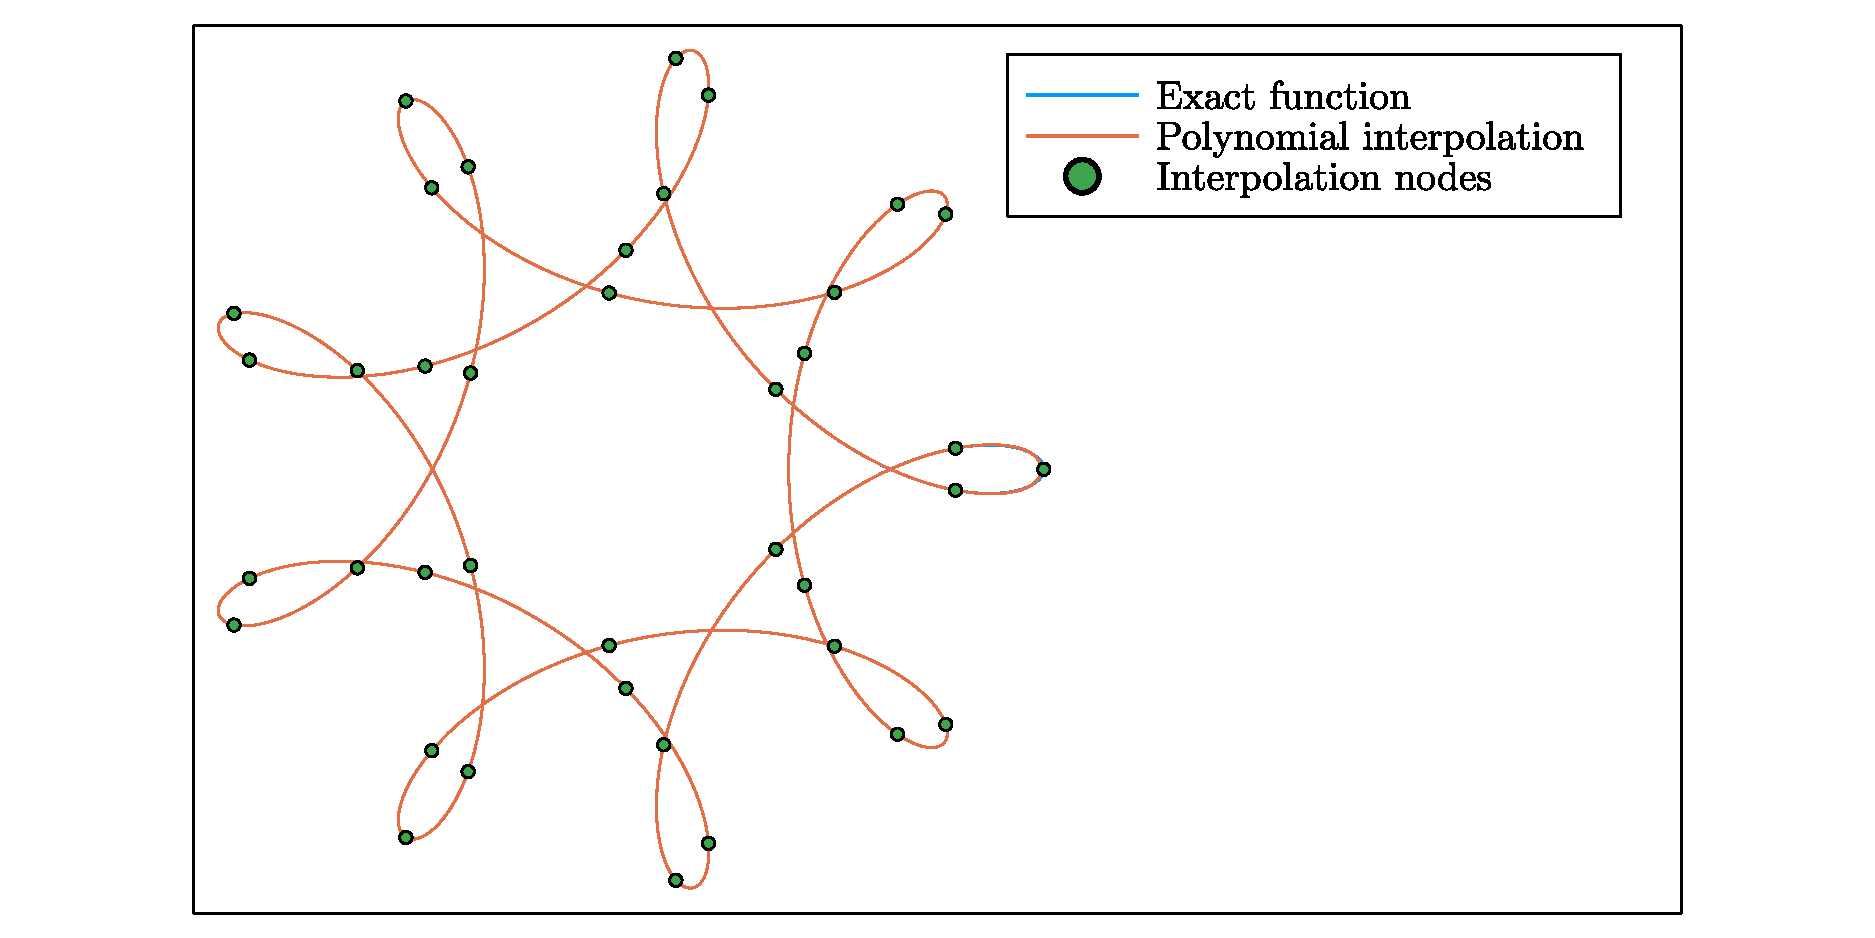
\includegraphics[width=0.99\linewidth]{figures/interpolation.pdf}
        \caption{Solution for \cref{exercise:parametric_interpolation}.}%
        \label{fig:parametric_interpolation}
    \end{figure}
\end{compexercise}

\begin{compexercise}
    [Solving the Laplace equation using a spectral method]
    The classical Laplace equation with homogeneous Dirichlet boundary conditions in dimension 1 reads
    \begin{equation}
        \label{eq:laplace}
        \text{Find $u \in C^2\bigl([0, 1]\bigr)$ such that}
        \qquad
        \left\{
        \begin{aligned}
        &- u''(x) = f(x) \qquad \forall x \in (0, 1), \\
        &u(0) = u(1) = 0.
        \end{aligned}
        \right.
    \end{equation}
    Our goal in this exercise is to approximate the exact solution~$u(x)$ using interpolation.
    Specifically,
    we propose to proceed in two steps:
    \begin{itemize}
        \item
            Interpolate the right-hand side using a polynomial with equidistant nodes.
            That is, find a polynomial $\widehat f \in \poly(n)$ such that
            \[
                \forall i \in \{0, \dotsc, n\}, \qquad
                \widehat f(x_i) = f(x_i), \qquad x_i = \frac{i}{n}.
            \]

        \item
            Solve~\eqref{eq:laplace} with $\widehat f$ instead of $f$.
            Since $\widehat f$ is a polynomial, this can be achieved analytically.
    \end{itemize}
    Implement this program in the case where
    \[
        f(x) = \exp\bigl(\sin(2\pi x)\bigr) \cos(2 \pi x)^2 - \exp\bigl(\sin(2 \pi x)\bigr)  \sin(2 \pi x),
    \]
    and compare for various values of~$n$ the approximate solution you obtain with
    the exact solution to~\eqref{eq:laplace},
    which is given by $u(x) = (2\pi)^{-2} \exp \bigl(\bigl( \sin(2\pi x) \bigr) - 1\bigr)$ in this case.
    % How does the maximum of the error over the interval $[0, 1]$?
\end{compexercise}

\begin{compexercise}
    [Modeling the vapor pressure of mercury]
    \label{exercise:approx}
    The dataset loaded through the following Julia commands contains data on the vapor pressure of mercury as a function of the temperature.
    \begin{minted}{julia}
    import RDatasets
    data = RDatasets.dataset("datasets", "pressure")
    \end{minted}
    Find a low-dimensional mathematical model of the form
    \begin{equation}
        p(T) = \exp \bigl( \alpha_0 + \alpha_1 T + \alpha_2 T^2 + \alpha_3 T^3 \bigr)
    \end{equation}
    for the pressure as a function of the temperature.
    Plot the approximation together with the data.
    An example solution is given in~\cref{fig:pressure}.
    \begin{figure}[ht]
        \centering
        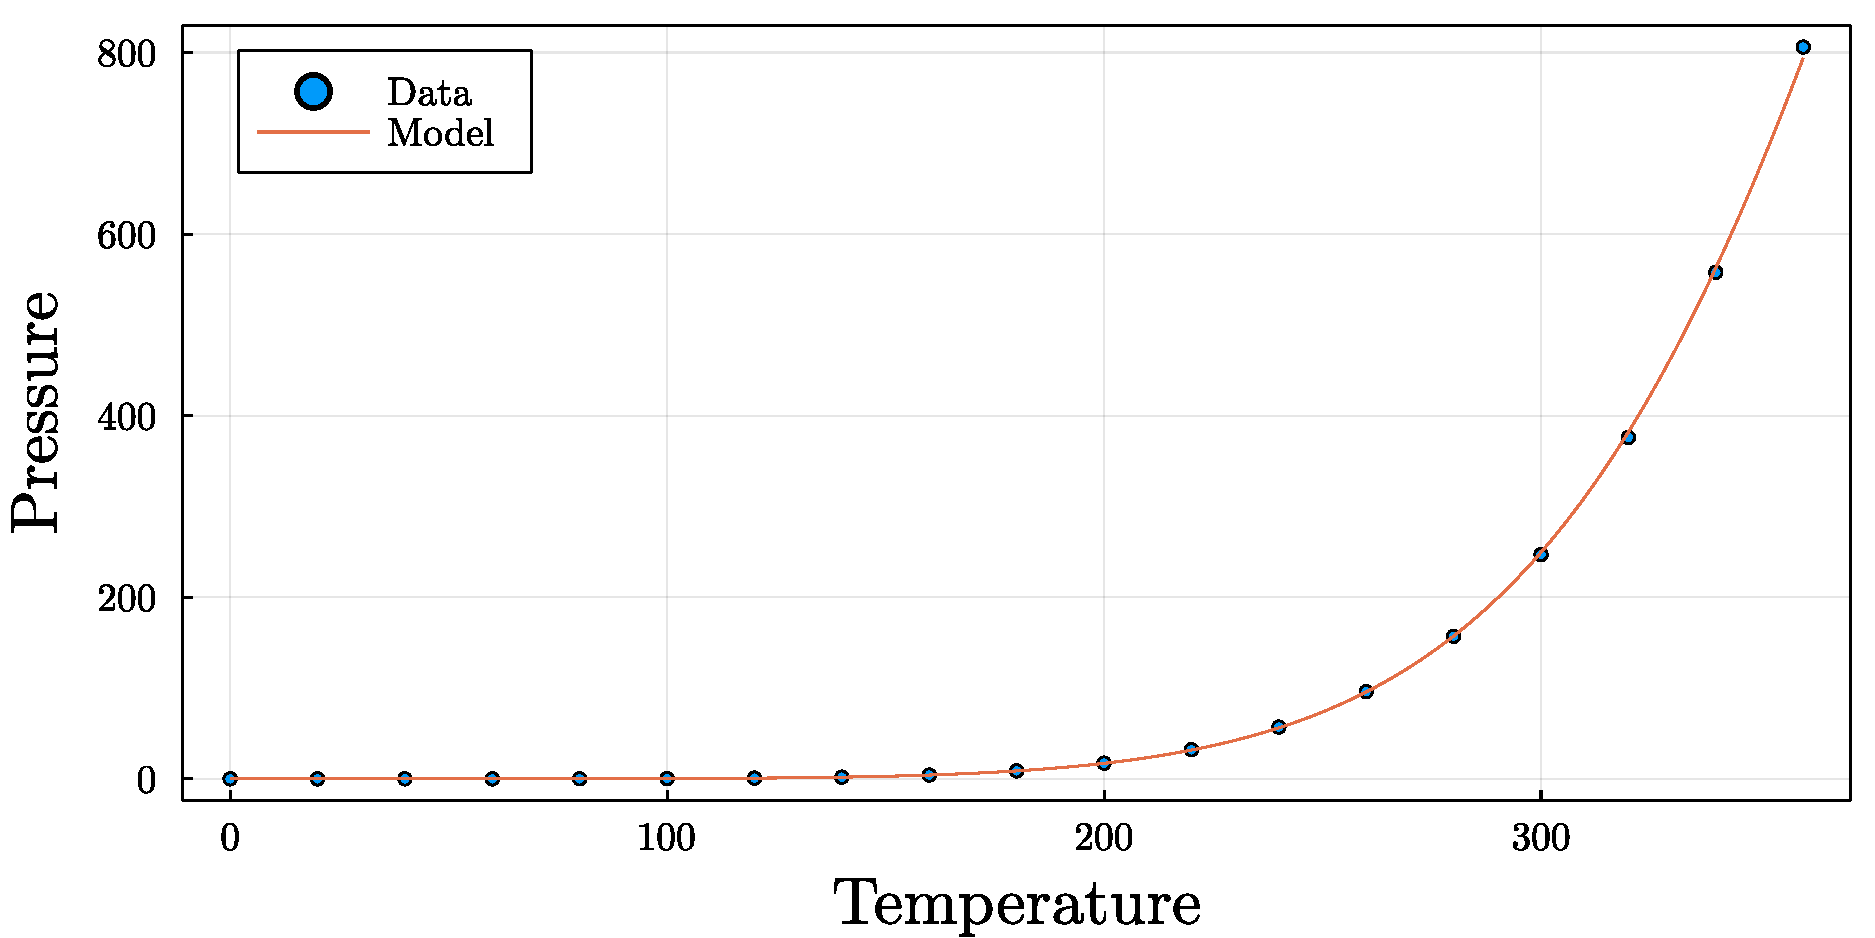
\includegraphics[width=0.75\linewidth]{figures/pressure_model.pdf}
        \caption{Solution for \cref{exercise:approx}.}%
        \label{fig:pressure}
    \end{figure}
\end{compexercise}

\begin{compexercise}
    \label{exercise:fourier_interp}
    Let $u\colon [0, 2\pi] \to \real$ and
    \begin{equation}
        \label{eq:interp_nodes_fourier}
        x_k = \left( \frac{2k\pi}{2n+1} \right), \qquad k = 0, \dotsc, 2n.
    \end{equation}
    We wish to interpolate $u$ at these nodes using complex exponentials:
    \[
        \widehat u = \sum_{k=-n}^{n} a_k \e^{\i k x}.
    \]
    Write a function
    \begin{minted}{julia}
        function fourier_interpolate(u, x, X)
            # Your code comes here ...
        end
    \end{minted}
    which takes three arguments:
    \begin{itemize}
        \item \julia{u} is the function to interpolate;

        \item \julia{x} are the interpolation nodes, given by~\eqref{eq:interp_nodes_fourier} in the test code below; 
            you can assume that this array contains an odd number of elements.

        \item \julia{X} is a one-dimensional of values on the $x$ axis.
    \end{itemize}
    The function should return a one-dimensional array containing the values taken by $\widehat u$ when evaluated at the points contained in \julia{X}.
    The can use the following code to test your function:
    \begin{minted}{julia}
    import Plots
    n, m = 5, 1000
    x = 2π/(2n+1) * (0:2n)
    X = 2π/m * (0:m)

    u(x) = sign(x - π)
    # u(x) = exp(sin(x) + cos(5x))
    # u(x) = x^2 * (x - 2π)^2 / π^4

    @time U = fourier_interpolate(u, x, X)
    Plots.plot(X, u.(X), label="u(x)", legend=:bottomright)
    Plots.plot!(X, U, label="û(x)")
    Plots.scatter!(x, u.(x), label="Interpolation points")
    Plots.xlims!(0, 2π)
    \end{minted}
    An example of the output plot is illustrated in~\cref{fig:fourier}.
\end{compexercise}
\begin{figure}[ht]
    \centering
    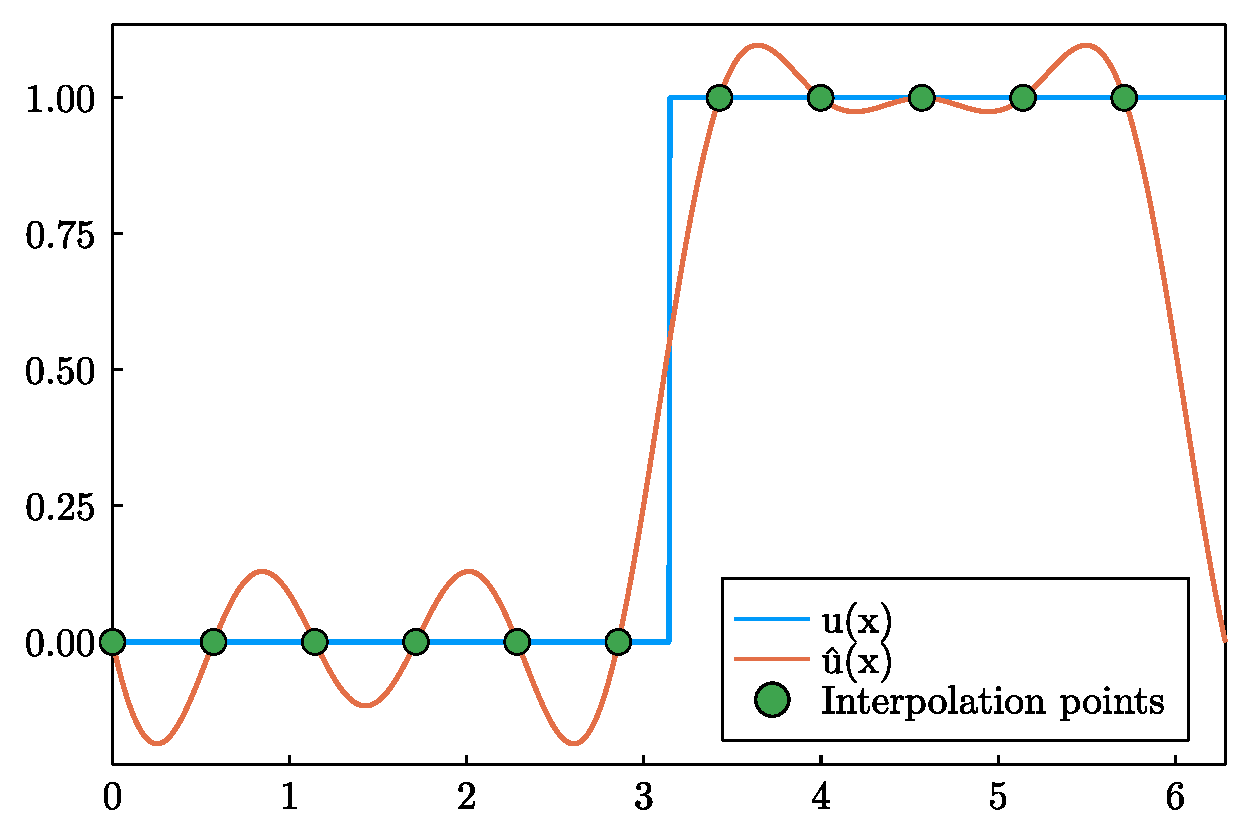
\includegraphics[width=0.8\linewidth]{figures/fourier.pdf}
    \caption{Example solution for~\cref{exercise:fourier_interp}.}%
    \label{fig:fourier}
\end{figure}

\section{Discussion and bibliography}
A comprehensive study of approximation theory would require to cover the $L^{\infty}$ setting
as well as other functional settings.
A pillar of $L^{\infty}$ approximation theorem is Chebyshev's equioscillation theorem, which we alluded to in~\cref{remark:cheb}.
An excellent introductory reference on approximation theory is~\cite{magnus} (in French).
See also~\cite[Chapter 10]{MR2265914} and the references therein.
%

\chapter{Numerical integration}
\label{cha:quadrature}

\nocite{*}
\printbibliography
\end{document}
